
\chapter{Physics}

\noindent
\textbf{Everything there is to know about physics} -- excerpted from ``Everything you need to know about school'' in the September 16, 2008 edition of the Seattle periodical \textit{The Stranger}:

\vskip 10pt {\narrower \noindent \baselineskip5pt

If stuff is still, it doesn't like to move; if stuff is moving, it doesn't like to stop.  The more stuff you are trying to move, the more you need to push it to speed it up.  When you push on stuff, it pushes back on you.  Stuff likes other stuff, from a distance at least.  Stuff likes becoming more chaotic, but cannot be created or destroyed; stuff can be rearranged.  (All that is Isaac Newton.)  Energy, like stuff, cannot be created or destroyed, only changed from one kind to another.  Energy can be stored in movement, bonds between stuff, and many other places.  Changes in how energy is stored allow us to do things -- like bake, drive, get up tall buildings, and kill each other.  (That's Sadi Carnot.)  Also, stuff \textit{is} energy.  Stuff is a lot of energy.  (That's Albert Einstein.)  Compress plutonium with explosives and the atoms fission, releasing the energy stored in stuff.  When the energy is released in downtown Nagasaki, you kill about 40,000 people right away and another 40,000 over time.  (Thanks, Enrico Fermi!)

\par} \vskip 10pt

\vskip 10pt

There is a lot of truth to this quote, despite its sarcastic tone.  Physics really is the study of matter and energy, and of the laws governing the interactions of both.  The movement of matter largely follows the laws described by Isaac Newton (so much so that this category of physics is often referred to as \textit{Newtonian physics}).  The flow and transformation of energy is a category called \textit{thermodynamics}.  Albert Einstein went on to equate matter with energy through his famous equation $E = mc^2$ which helped usher in the age of nuclear physics.

Physics is important to the study of industrial instrumentation because its laws describe and explain so many applications of measurement and control.  As a teacher, one of the things I like to tell students is that their chosen field is really nothing more than applied physics.  Granted, there aren't too many applications of macroscopic projectile motion in industrial measurement and control, but on a microscopic level this is what all moving fluids are: an extremely large collection of independent molecules obeying Newtonian laws of motion.  Physics is the study of \textit{stuff}, while instrumentation is the discipline of measuring and controlling stuff.  The better you understand stuff, the better you will be able to measure and control that stuff.  Enjoy!







\filbreak
\section{Terms and Definitions}

\textit{Mass} ($m$) is the opposition an object has to acceleration (changes in velocity).  \textit{Weight} is the force ($F$) imposed on a mass by a gravitational field.  Mass is an intrinsic property of an object, regardless of the environment.  Weight, on the other hand, depends on the strength of the gravitational field in which the object resides.  A 20 kilogram slug of metal has the exact same mass whether it rests on Earth, or in the zero-gravity environment of outer space, or on the surface of the planet Jupiter.  However, the \textit{weight} of that mass depends on gravity: zero weight in outer space (where there is no gravity to act upon it), some weight on Earth, and a much greater amount of weight on the planet Jupiter (due to the much stronger gravitational field of that planet).

Since mass is the opposition of an object to changes in velocity (acceleration), it stands to reason force, mass, and acceleration for any particular object are directly related to one another:

$$F = ma$$

\noindent
Where,

$F$ = Force in newtons (metric) or pounds (British)

$m$ = Mass in kilograms (metric) or slugs (British)

$a$ = Acceleration in meters per second squared (metric) or feet per second squared (British)

\vskip 10pt

If the force in question is the weight of the object, then the acceleration ($a$) in question is the acceleration constant of the gravitational field where the object resides.  For Earth at sea level, $a_{gravity}$ is approximately 9.81 meters per second squared, or 32.2 feet per second squared.  Earth's gravitational acceleration constant is usually represented in equations by the variable letter $g$ instead of the more generic $a$.

Since acceleration is nothing more than the rate of velocity change with respect to time, the force/mass equation may be expressed using the calculus notation of the first derivative:

$$F = m{dv \over dt}$$

\noindent
Where,

$F$ = Force in newtons (metric) or pounds (British)

$m$ = Mass in kilograms (metric) or slugs (British)

$v$ = Velocity in meters per second (metric) or feet per second (British)

$t$ = Time in seconds

\vskip 10pt

Since velocity is nothing more than the rate of position change with respect to time, the force/mass equation may be expressed using the calculus notation of the second derivative (acceleration being the derivative of velocity, which in turn is the derivative of position):

$$F = m{d^2x \over dt^2}$$

\noindent
Where,

$F$ = Force in newtons (metric) or pounds (British)

$m$ = Mass in kilograms (metric) or slugs (British)

$x$ = Position in meters (metric) or feet (British)

$t$ = Time in seconds

\vskip 10pt


\textit{Mass density} ($\rho$) for any substance is the proportion of mass to volume.  \textit{Weight density} ($\gamma$) for any substance is the proportion of weight to volume. \index{Mass density}  \index{Weight density}

Just as weight and mass are related to each other by gravitational acceleration, weight density and mass density are also related to each other by gravity:

$$F_{weight} = mg \hbox{\hskip 20pt Weight and Mass}$$

$$\gamma = \rho g \hbox{\hskip 20pt Weight density and Mass density}$$







\filbreak
\section{Metric prefixes}

$$\includegraphics{002.eps}$$








\filbreak
\section{Areas and volumes}

\textit{Area} refers to the size of two-dimensional surface.  \textit{Volume} refers to the size of a three-dimensional space.  To put both these measures into context; the question of how much paint will be required to adequately cover a house is one of area, while the question of how much water will be required to fill a pond is one of volume.  \index{Area, defined}  \index{Volume, defined}

Some units of measurement for area and volume are nothing more than compounded linear units.  Ten \textit{centimeters} is an expression of distance, while ten \textit{square centimeters} (cm$^{2}$) is an expression of area, and ten \textit{cubic centimeters} (cm$^{3}$) is an expression of volume.  It important to note that the modifiers ``square'' and ``cubic'' do not in any way imply the object in question is square or cubic in shape.  It is perfectly reasonable to measure the area of a \textit{circle}, for instance, using the unit of \textit{square} centimeters.

\vskip 10pt

Other units of spatial measurement are specific to area or to volume.  The \textit{acre}, for example, is a unit of area measurement developed for the purpose of quantifying the size of land plots, one acre being equivalent to 43560 square feet.  An example of a unit specifically devoted to volume measurement is the \textit{liter}, equivalent to 1000 cubic centimeters. \index{Acre, defined}





\filbreak
\subsection{Common geometric shapes}

$$\includegraphics{shapes_05.eps}$$

$$\includegraphics{shapes_01.eps}$$

$$\includegraphics{shapes_02.eps}$$

\filbreak

$$\includegraphics{shapes_03.eps}$$

$$\includegraphics{shapes_04.eps}$$







\filbreak
\section{Unit conversions and physical constants}

\label{Unit conversions}

Converting between disparate units of measurement is the bane of many science students.  The problem is worse for students in the United States of America, who must work with British (``Customary'') units such as the pound, the foot, the gallon, etc.  World-wide adoption of the metric system would go a long way toward alleviating this problem, but until then it is important for students to master the art of unit conversions\footnote{An interesting point to make here is the United States did get something right when they designed their monetary system of dollars and cents.  This is essentially a \textit{metric} system of measurement, with 100 cents per dollar.  The founders of the USA wisely decided to avoid the utterly confusing denominations of the British, with their pounds, pence, farthings, shillings, etc.  The denominations of penny, dime, dollar, and eagle (\$10 gold coin) comprised a simple power-of-ten system for money.  Credit goes to France for first adopting a metric system of general weights and measures as their national standard.}.

It is possible to convert from one unit of measurement to another by use of tables designed expressly for this purpose.  Such tables usually have a column of units on the left-hand side and an identical row of units along the top, whereby one can look up the conversion factor to multiply by to convert from any listed unit to any other listed unit.  While such tables are undeniably simple to use, they are practically impossible to memorize.

A better way to convert between different units is shown in the next subsection.












\filbreak
\subsection{Unity fractions}

An important principle in the physical sciences is to closely track all units of measurement when performing calculations of physical quantities.  This practice is generally referred to as \textit{dimensional analysis}.  A brief example of dimensional analysis is shown here, used to analyze the simple formula $P = IV$ which describes the amount of power dissipated by an electrical load ($P$) given its current ($I$) and voltage drop ($V$):  \index{Dimensional analysis}

$$P = IV$$

Substituting units of measurement for each variable in this formula (i.e. Watts for power, Amperes for current, and Volts for voltage), using bracket symbols to denote these as unit abbreviations rather than variables, we get this result:

$$[\hbox{Watts}] = [\hbox{Amperes}] \times [\hbox{Volts}] \hbox{\hskip 20pt or \hskip 20pt} [\hbox{W}] = [\hbox{A}] [\hbox{V}]$$

If we happen to know that ``watts'' is equivalent to joules of energy dissipated per second, and that ``amperes'' is equivalent to coulombs of charge motion per second, and that ``volts'' is equivalent to joules of energy per coulomb of electrical charge, we may substitute these units of measurement into the formula and see that the unit of ``coulomb'' cancels just like identical variables in the numerator and denominator of multiplied fractions:

$$\left[\hbox{Joules} \over \hbox{Seconds} \right] = \left[\hbox{\sout{Coulombs}} \over \hbox{Seconds}\right] \times \left[\hbox{Joules} \over \hbox{\sout{Coulombs}}\right] \hbox{\hskip 20pt or \hskip 20pt} \left[\hbox{J} \over \hbox{s} \right] = \left[\hbox{\sout{C}} \over \hbox{s} \right] \left[\hbox{J} \over \hbox{\sout{C}} \right]$$

\vskip 10pt

As it so happens, dimensional analysis may be employed in a similar manner to convert between different units of measurement via a technique I like to call \textit{unity fractions}. \index{Unit conversions} \index{Unity fraction}

This technique involves setting up the original quantity as a fraction, then multiplying by a series of fractions having \textit{physical} values of unity (1) so that by multiplication the original value does not change, but the units do.  Let's take for example the conversion of quarts into gallons, an example of a fluid volume conversion:

$$35 \hbox{ qt} = \hbox{??? gal}$$

Now, most people know there are four quarts in one gallon, and so it is tempting to simply divide the number 35 by four to arrive at the proper number of gallons.  However, the purpose of this example is to show you how the technique of unity fractions works, not to get an answer to a problem.  

\vskip 10pt

\filbreak

To demonstrate the unity fraction technique, we will first write the original quantity as a fraction, in this case a fraction with 1 as the denominator:

$${35 \hbox{ qt} \over 1}$$

Next, we will multiply this fraction by another fraction having a \textit{physical} value of unity (1) so that we do not alter\footnote{A basic mathematical identity is that multiplication of any quantity by 1 does not change the value of that original quantity.  If we multiply some quantity by a fraction having a physical value of 1, no matter how strange-looking that fraction may appear, the value of the original quantity will be left intact.  The goal here is to judiciously choose a fraction with a physical value of 1 but with its units of measurement so arranged that we cancel out the original quantity's unit(s) and replace them with the units we desire.} the quantity.  This means a fraction comprised of equal measures in the numerator and denominator, but having different units of measurement.  This ``unity'' fraction must be arranged in such a way that the undesired unit cancels out and leaves only the desired unit(s) in the product.  In this particular example, we wish to cancel out quarts and end up with gallons, so we must arrange a fraction consisting of quarts and gallons having equal quantities in numerator and denominator, such that quarts will cancel and gallons will remain:

$$\left({35 \hbox{ qt} \over 1}\right) \left({1 \hbox{ gal} \over 4 \hbox{ qt}}\right)$$

Now we see how the unit of ``quarts'' cancels from the numerator of the first fraction and the denominator of the second (``unity'') fraction, leaving only the unit of ``gallons'' left standing:

$$\left({35 \hbox{ \sout{qt}} \over 1}\right) \left({1 \hbox{ gal} \over 4 \hbox{ \sout{qt}}}\right) = 8.75 \hbox{ gal}$$

The reason this conversion technique is so powerful is it allows one to perform the largest range of unit conversions while memorizing the smallest possible set of conversion factors.

\vskip 10pt

Here is a set of six equal volumes, each one expressed in a different unit of measurement:

\vskip 10pt

\noindent
\textit{1 gallon (gal) = 231.0 cubic inches (in$^{3}$) = 4 quarts (qt) = 8 pints (pt) = 128 fluid ounces (fl. oz.) = 3.7854 liters (l)}

\vskip 10pt

Since all six of these quantities are physically equal, it is possible to build a ``unity fraction'' out of any two, to use in converting any of the represented volume units into any of the other represented volume units.  Shown here are a few different volume unit conversion problems, using unity fractions built only from these factors (all canceled units shown using strike-out lines):

\vskip 10pt

\noindent
40 gallons converted into fluid ounces (using \textit{128 fl. oz. = 1 gal} in the unity fraction):

$$\left({40 \hbox{ \sout{gal}} \over 1}\right) \left({128 \hbox{ fl. oz.} \over 1 \hbox{ \sout{gal}}}\right) = 5120 \hbox{ fl. oz}$$

\vskip 10pt

\noindent
5.5 pints converted into cubic inches (using \textit{231 in$^{3}$ = 8 pt} in the unity fraction):

$$\left({5.5 \hbox{ \sout{pt}} \over 1}\right) \left({231 \hbox{ in}^3 \over 8 \hbox{ \sout{pt}}}\right) = 158.8 \hbox{ in}^3$$

\vskip 10pt

\noindent
1170 liters converted into quarts:

$$\left({1170 \hbox{ \sout{l}} \over 1}\right) \left({4 \hbox{ qt} \over 3.7854 \hbox{ \sout{l}}}\right) = 1236 \hbox{ qt}$$

\vskip 10pt

By contrast, if we were to try to memorize a 6 $\times$ 6 table giving conversion factors between \textit{any two} of six volume units, we would have to commit 30 different conversion factors to memory!  Clearly, the ability to set up ``unity fractions'' is a much more memory-efficient and practical approach.

\vskip 10pt

This economy of conversion factors is very useful, and may also be extended to cases where linear units are raised to powers to represent two- or three-dimensional quantities.  To illustrate, suppose we wished to convert 5.5 pints into cubic \textit{feet} instead of cubic \textit{inches}: with no conversion equivalence between pints and cubic feet included in our string of six equalities, what do we do?

We should know the equality between inches and feet: there are exactly 12 inches in 1 foot.  This simple fact may be applied by incorporating \textit{another} unity fraction in the original problem to convert cubic inches into cubic feet.  We will begin by including another unity fraction comprised of 12 inches and 1 foot,just to see how this might work:

\vskip 10pt

\noindent
5.5 pints converted into cubic feet (\textit{our first attempt!}):

$$\left({5.5 \hbox{ \sout{pt}} \over 1}\right) \left({231 \hbox{ in}^3 \over 8 \hbox{ \sout{pt}}}\right) \left(1 \hbox{ ft} \over 12 \hbox{ \sout{in}}\right) = 13.23 \hbox{ in}^2 \cdot \hbox{ft}$$

\vskip 10pt

Unfortunately, this yields a non-sensical unit of square inch-feet.  Even though ${1 \hbox{ ft} \over 12 \hbox{ in}}$ is a valid unity fraction, it does not \textit{completely} cancel out the unit of cubic inches in the numerator of the first unity fraction.  Instead, the unit of ``inches'' in the denominator of the unity fraction merely cancels out one of the ``inches'' in the ``cubic inches'' of the previous fraction's numerator, leaving square inches (in$^{2}$).  What we need for full cancellation of cubic inches is a unity fraction relating \textit{cubic} feet to \textit{cubic} inches.  We can get this, though, simply by \textit{cubing} the ${1 \hbox{ ft} \over 12 \hbox{ in}}$ unity fraction:

\vskip 10pt

\noindent
5.5 pints converted into cubic feet (\textit{our second attempt!}):

$$\left({5.5 \hbox{ pt} \over 1}\right) \left({231 \hbox{ in}^3 \over 8 \hbox{ pt}}\right) \left(1 \hbox{ ft} \over 12 \hbox{ in}\right)^3$$

Distributing the third power to the interior terms of the last unity fraction:

$$\left({5.5 \hbox{ pt} \over 1}\right) \left({231 \hbox{ in}^3 \over 8 \hbox{ pt}}\right) \left(1^3 \hbox{ ft}^3 \over 12^3 \hbox{ in}^3\right)$$

Calculating the values of $1^3$ and $12^3$ inside the last unity fraction, then canceling units and solving:

$$\left({5.5 \hbox{ \sout{pt}} \over 1}\right) \left({231 \hbox{ \sout{in}}^3 \over 8 \hbox{ \sout{pt}}}\right) \left(1 \hbox{ ft}^3 \over 1728 \hbox{ \sout{in}}^3\right) = 0.0919 \hbox{ ft}^3$$

Now the answer makes sense: a volume expressed in units of cubic feet.

\vskip 10pt

\filbreak

Once again, this unit conversion technique shows its power by minimizing the number of conversion factors we must memorize.  We need not memorize how many cubic inches are in a cubic foot, or how many square inches are in a square foot, if we know how many linear inches are in a linear foot and we simply let the fractions ``tell'' us whether a power is needed for unit cancellation.

\vskip 10pt

Unity fractions are also useful when we need to convert more than one unit in a given quantity.  For example, suppose a flowmeter at a wastewater treatment facility gave us a flow measurement of 205 cubic feet per minute but we needed to convert this expression of water flow into units of cubic yards per day.  Observe the following unit-fraction conversion to see how unity fractions serve the purpose of converting cubic feet into cubic yards, and minutes into days (by way of minutes to hours, and hours to days):

$$\left(205 \hbox{ \sout{ft}}^3 \over \hbox{\sout{min}} \right) \left(1^3 \hbox{ yd}^3 \over 3^3 \hbox{ \sout{ft}}^3\right) \left(60 \hbox{ \sout{min}} \over 1 \hbox{ \sout{hr}}\right) \left(24 \hbox{ \sout{hr}} \over 1 \hbox{ day}\right) = 10933.3 \hbox{ yd}^3\hbox{/day}$$

Note how the only units left un-canceled on the left-hand side of the ``equals'' symbol are cubic yards (yd$^{3}$) and days, which therefore become the units of measurement for the final result.

\vskip 10pt

A major caveat to this method of converting units is that the units must be \textit{directly proportional} to one another, since this multiplicative conversion method is really nothing more than an exercise in mathematical proportions.  Here are some examples (but not an exhaustive list!) of conversions that \textit{cannot} be performed using the ``unity fraction'' method:

\begin{itemize}
\item Absolute / Gauge pressures, because one scale is \textit{offset} from the other by 14.7 PSI (atmospheric pressure).
\item Celsius / Fahrenheit, because one scale is \textit{offset} from the other by 32 degrees.
\item Wire diameter / gauge number, because gauge numbers grow smaller as wire diameter grows larger (inverse proportion rather than direct) and because there is no proportion relating the two.
\item Power / decibels, because the relationship is logarithmic rather than proportional.
\end{itemize}

\vskip 10pt

The following subsections give sets of physically equal quantities, which may be used to create unity fractions for unit conversion problems.  Note that only those quantities shown in the same line (separated by $=$ symbols) are truly equal to each other, not quantities appearing in different lines!



\filbreak
\subsection{Conversion formulae for temperature}

Note: all of the conversion factors given for temperature are \textit{exact}, not approximations.

\vskip 10pt

\noindent
$^{o}$F = ($^{o}$C)(9/5) + 32

\noindent
$^{o}$C = ($^{o}$F $-$ 32)(5/9)

\noindent
$^{o}$R = $^{o}$F + 459.67

\noindent
K = $^{o}$C + 273.15




\filbreak
\subsection{Conversion factors for distance}

Note: all of the conversion factors given for distance are \textit{exact}, not approximations.

\vskip 10pt

\noindent
\textbf{1 inch} (in) = \textbf{2.54 centimeters} (cm)

\noindent
\textbf{1 foot} (ft) = \textbf{12 inches} (in)

\noindent
\textbf{1 yard} (yd) = \textbf{3 feet} (ft)

\noindent
\textbf{1 mile} (mi) = \textbf{5280 feet} (ft)




\filbreak
\subsection{Conversion factors for volume}

Note: all conversion factors shown in \textbf{bold} type are \textit{exact}, not approximations.

\vskip 10pt

\noindent
\textbf{1 gallon} (gal) = 231.0 cubic inches (in$^{3}$) = \textbf{4 quarts} (qt) = \textbf{8 pints} (pt) = \textbf{16 cups} = \textbf{128 fluid ounces} (fl. oz.) = 3.7854 liters (l)

\vskip 10pt

\noindent
\textbf{1 milliliter} (ml) = \textbf{1 cubic centimeter} (cm$^{3}$)




\filbreak
\subsection{Conversion factors for velocity}

Note: all conversion factors shown in \textbf{bold} type are \textit{exact}, not approximations.

\vskip 10pt

\noindent 
\textbf{1 mile per hour} (mi/h) = \textbf{88 feet per minute} (ft/m) = 1.46667 feet per second (ft/s) = 1.60934 kilometer per hour (km/h) = 0.44704 meter per second (m/s) = 0.868976 knot (knot -- international)





\filbreak
\subsection{Conversion factors for mass}

\noindent 
1 pound-mass (lbm) = 0.4535924 kilogram (kg) = 0.031081 slugs




\filbreak
\subsection{Conversion factors for force}

\noindent 
1 pound-force (lbf) = 4.448222 newtons (N)

\vskip 10pt

\noindent 
\textbf{1 kilogram-force} (kgf) = \textbf{9.80665 newtons} (N)




\filbreak
\subsection{Conversion factors for area}

Note: all conversion factors shown in \textbf{bold} type are \textit{exact}, not approximations.

\vskip 10pt

\noindent 
1 acre = 43560 square feet (ft$^{2}$) = 4840 square yards (yd$^{2}$) = 4046.86 square meters (m$^{2}$)





\filbreak
\subsection{Conversion factors for pressure (either all gauge or all absolute)}

Note: all conversion factors shown in \textbf{bold} type are \textit{exact}, not approximations.

\vskip 10pt

\noindent 
1 pounds per square inch (PSI) = 2.03602 inches of mercury at 0 $^{o}$C (in. Hg) = 27.6799 inches of water at 4 $^{o}$C (in. W.C.) = 6.894757 kilopascals (kPa) = 0.06894757 bar

\vskip 10pt

\noindent 
\textbf{1 bar} = \textbf{100 kilopascals} (kPa) = 14.504 pounds per square inch (PSI)

\vskip 10pt

\noindent 
\textbf{1 meter of water at 4 $^{o}$C} (m W.C.) = \textbf{9.80665 kilopascals} (kPa)





\filbreak
\subsection{Conversion factors for pressure (absolute pressure units only)}

Note: all conversion factors shown in \textbf{bold} type are \textit{exact}, not approximations.

\vskip 10pt

\noindent 
\textbf{1 standard atmosphere} (Atm) = 14.7 pounds per square inch absolute (PSIA) = \textbf{101.325 kilopascals absolute} (kPaA) = \textbf{1.01325 bar absolute} = 760 millimeters of mercury absolute (mmHgA) = 760 torr (torr)





\filbreak
\subsection{Conversion factors for energy or work}

\noindent 
1 British thermal unit (Btu -- ``International Table'') = 251.996 calories (cal -- ``International Table'') = 1055.06 joules (J) = 1055.06 watt-seconds (W-s) = 0.293071 watt-hour (W-hr) = 1.05506 x 10$^{10}$ ergs (erg) = 778.169 foot-pound-force (ft-lbf) 





\filbreak
\subsection{Conversion factors for power}

Note: all conversion factors shown in \textbf{bold} type are \textit{exact}, not approximations.

\vskip 10pt

\noindent 
\textbf{1 horsepower} = \textbf{550 foot-pounds per second} (ft-lbf/s) = 745.7 watts (W) = 2544.43 British thermal units per hour (Btu/h) = 0.0760181 boiler horsepower (hp -- boiler)





\filbreak
\subsection{Terrestrial constants}

\noindent 
Acceleration of gravity at sea level = 9.806650 meters per second per second (m/s$^{2}$) = 32.1740 feet per second per second (ft/s$^{2}$)

\vskip 5pt

\noindent 
Atmospheric pressure = 14.7 pounds per square inch absolute (PSIA) = 760 millimeters of mercury absolute (mmHgA) = 760 torr (torr) = 1.01325 bar (bar)

\vskip 5pt

\noindent 
Atmospheric gas concentrations (by volume, not mass):

\begin{itemize}
\item Nitrogen = 78.084 \%
\item Oxygen = 20.946 \%
\item Argon = 0.934 \%
\item Carbon Dioxide (CO$_{2}$) = 0.033 \%
\item Neon = 18.18 ppm
\item Helium = 5.24 ppm
\item Methane (CH$_{4}$) = 2 ppm
\item Krypton = 1.14 ppm
\item Hydrogen = 0.5 ppm
\item Nitrous Oxide (N$_{2}$O) = 0.5 ppm
\item Xenon = 0.087 ppm
\end{itemize}

\vskip 10pt

\noindent
Density of dry air at 20 $^{o}$C and 760 torr = 1.204 mg/cm$^{3}$ = 1.204 kg/m$^{3}$ = 0.075 lb/ft$^{3}$ = 0.00235 slugs/ft$^{3}$

\vskip 5pt

\noindent
Absolute viscosity of dry air at 20 $^{o}$C and 760 torr = 0.018 centipoise (cp) = 1.8 $\times$ $10^{-5}$ pascal-seconds (Pa$\cdot$s)







\filbreak
\subsection{Properties of water}

\noindent
Freezing point at sea level = 32 $^{o}$F = 0 $^{o}$C

\vskip 5pt

\noindent
Boiling point at sea level = 212 $^{o}$F = 100 $^{o}$C

\vskip 5pt

\noindent
Density of water at 4 $^{o}$C = 1000 kg/m$^{3}$ = 1 g/cm$^{3}$ = 1 kg/liter = 62.428 lb/ft$^{3}$ = 1.94 slugs/ft$^{3}$

\vskip 5pt

\noindent
Specific heat of water at 14 $^{o}$C = 1.00002 calories/g$\cdot$$^{o}$C = 1 BTU/lb$\cdot$$^{o}$F = 4.1869 joules/g$\cdot$$^{o}$C

\vskip 5pt

\noindent
Specific heat of ice $\approx$ 0.5 calories/g$\cdot$$^{o}$C

\vskip 5pt

\noindent
Specific heat of steam $\approx$ 0.48 calories/g$\cdot$$^{o}$C

\vskip 5pt

\noindent
Absolute viscosity of water at 20 $^{o}$C = 1.0019 centipoise (cp) = 0.0010019 pascal-seconds (Pa$\cdot$s)

\vskip 5pt

\noindent
Surface tension of water (in contact with air) at 18 $^{o}$C = 73.05 dynes/cm

\vskip 5pt

\noindent
pH of pure water at 25 $^{o}$C = 7.0 (\textit{pH scale = 0 to 14})






\filbreak
\subsection{Miscellaneous physical constants}

Note: all constants shown in \textbf{bold} type are \textit{exact}, not approximations.  Parentheses show one standard deviation ($\sigma$) of uncertainty in the last digits: for example, Avogadro's number given as 6.02214179(30) $\times$ $10^{23}$ means the center value ($6.02214179 \times 10^{23}$) plus or minus $0.00000030 \times 10^{23}$.

\vskip 10pt

\noindent 
Avogadro's number ($N_A$) = 6.02214179(30) $\times$ $10^{23}$ per mole (mol$^{-1}$)

\vskip 5pt

\noindent
Boltzmann's constant ($k$) = 1.3806504(24) $\times$ $10^{-23}$ joules per Kelvin (J/K)

\vskip 5pt

\noindent
Electronic charge ($e$) = 1.602176487(40) $\times$ $10^{-19}$ Coulomb (C)

\vskip 5pt

\noindent
Faraday constant ($F$) = 9.64853399(24) $\times$ $10^{4}$ Coulombs per mole (C/mol)

\vskip 5pt

\noindent
Gravitational constant ($G$) = 6.67428(67) $\times$ $10^{-11}$ cubic meters per kilogram-seconds squared (m$^{3}$/kg-s$^{2}$)

\vskip 5pt

\noindent 
Molar gas constant ($R$) = 8.314472(15) joules per mole-Kelvin (J/mol-K) = 0.08205746(14) liters-atmospheres per mole-Kelvin

\vskip 5pt

\noindent 
Planck constant ($h$) = 6.62606896(33) $\times$ $10^{-34}$ joule-seconds (J-s)

\vskip 5pt

\noindent
Stefan-Boltzmann constant ($\sigma$) = 5.670400(40) $\times$ $10^{-8}$ Watts per square meter-Kelvin$^{4}$ (W/m$^{2} \cdot$K$^{4}$)

\vskip 5pt

\noindent 
Speed of light in a vacuum ($c$) = \textbf{299792458 meters per second} (m/s) = 186282.4 miles per second (mi/s)

\vskip 10pt

\noindent
All constants taken from NIST data ``Fundamental Physical Constants -- Extensive Listing'', published 2006.







\filbreak
\subsection{Weight densities of common materials}

All density figures approximate for samples at standard temperature and pressure\footnote{Density figures taken or derived from tables in the \textit{CRC Handbook of Chemistry and Physics}, 64th Edition.  Most liquid densities taken from table on page F-3 and solid densities taken from table on page F-1.  Some liquid densities taken from tables on pages E-27 through E-31.  All temperatures at or near 20 $^{o}$C.}.

\subsubsection{Liquids:}

\begin{itemize}
\item Acetone: $\gamma$ = 49.4 lb/ft$^{3}$
\item Alcohol, ethyl (ethanol): $\gamma$ = 49.4 lb/ft$^{3}$
\item Alcohol, methyl (methanol): $\gamma$ = 50.5 lb/ft$^{3}$
\item Benzene: $\gamma$ = 56.1 lb/ft$^{3}$
\item Butane (liquid): $\gamma$ = 36.1 lb/ft$^{3}$
\item Carbon disulfide: $\gamma$ = 80.7 lb/ft$^{3}$
\item Carbon tetrachloride: $\gamma$ = 99.6 lb/ft$^{3}$
\item Chloroform: $\gamma$ = 93 lb/ft$^{3}$
\item Ethylene glycol (ethanediol): $\gamma$ = 69.22 lb/ft$^{3}$
\item Gasoline: $\gamma$ = 41 lb/ft$^{3}$ to 43 lb/ft$^{3}$
\item Glycerin: $\gamma$ = 78.6 lb/ft$^{3}$
\item Isobutane (liquid): $\gamma$ = 34.8 lb/ft$^{3}$
\item Kerosene: $\gamma$ = 51.2 lb/ft$^{3}$
\item Mercury: $\gamma$ = 849 lb/ft$^{3}$
\item Methanol (methyl alcohol): $\gamma$ = 50.5 lb/ft$^{3}$
\item Milk: $\gamma$ = 64.2 lb/ft$^{3}$ to 64.6 lb/ft$^{3}$
\item Naphtha, petroleum: $\gamma$ = 41.5 lb/ft$^{3}$
\item Oil, castor: $\gamma$ = 60.5 lb/ft$^{3}$
\item Oil, coconut: $\gamma$ = 57.7 lb/ft$^{3}$
\item Oil, linseed (boiled): $\gamma$ = 58.8 lb/ft$^{3}$
\item Oil, olive: $\gamma$ = 57.3 lb/ft$^{3}$
\item Propane (liquid): $\gamma$ = 31.2 lb/ft$^{3}$
\item Toluene: $\gamma$ = 54.1 lb/ft$^{3}$
\item Turpentine: $\gamma$ = 54.3 lb/ft$^{3}$
\item Water, heavy: $\gamma$ = 68.97 lb/ft$^{3}$
\item Water, light (normal): $\gamma$ = 62.4 lb/ft$^{3}$
\item Water, sea: $\gamma$ = 63.99 lb/ft$^{3}$
\end{itemize}

\subsubsection{Solids:}

\begin{itemize}
\item Beryllium: $\gamma$ = 115.37 lb/ft$^{3}$
\item Brass: $\gamma$ = 524.4 lb/ft$^{3}$
\item Calcium: $\gamma$ = 96.763 lb/ft$^{3}$
\item Carbon (diamond): $\gamma$ = 196.65 lb/ft$^{3}$ to 220.37 lb/ft$^{3}$
\item Cement (set): $\gamma$ = 170 lb/ft$^{3}$ to 190 lb/ft$^{3}$ 
\item Chromium: $\gamma$ = 448.86 lb/ft$^{3}$
\item Copper: $\gamma$ = 559.36 lb/ft$^{3}$
\item Cork: $\gamma$ = 14 lb/ft$^{3}$ to 16 lb/ft$^{3}$
\item Gold: $\gamma$ = 1178.6 lb/ft$^{3}$
\item Ice: $\gamma$ = 57.2 lb/ft$^{3}$
\item Iron: $\gamma$ = 490.68 lb/ft$^{3}$
\item Ivory: $\gamma$ = 114 lb/ft$^{3}$ to 120 lb/ft$^{3}$
\item Lead: $\gamma$ = 708.56 lb/ft$^{3}$
\item Leather: $\gamma$ = 54 lb/ft$^{3}$
\item Magnesium: $\gamma$ = 108.50 lb/ft$^{3}$
\item Molybdenum: $\gamma$ = 638.01 lb/ft$^{3}$
\item Quartz: $\gamma$ = 165 lb/ft$^{3}$
\item Rubber (soft): $\gamma$ = 69 lb/ft$^{3}$
\item Rubber (hard): $\gamma$ = 74 lb/ft$^{3}$
\item Salt, rock: $\gamma$ = 136 lb/ft$^{3}$
\item Sugar: $\gamma$ = 99 lb/ft$^{3}$
\item Tar: $\gamma$ = 66 lb/ft$^{3}$
\item Wood, balsa: $\gamma$ = 7 lb/ft$^{3}$ to 9 lb/ft$^{3}$
\item Wood, maple: $\gamma$ = 39 lb/ft$^{3}$ to 47 lb/ft$^{3}$
\end{itemize}










\filbreak
\section{Dimensional analysis}

An interesting parallel to the ``unity fraction'' unit conversion technique is something referred to in physics as \textit{dimensional analysis}.  Performing dimensional analysis on a physics formula means to set it up with units of measurement in place of variables, to see how units cancel and combine to form the appropriate unit(s) of measurement for the result.  \index{Dimensional analysis}

For example, let's take the familiar power formula used to calculate power in a simple DC electric circuit:

$$P = IV$$

\noindent
Where,

$P$ = Power (watts)

$I$ = Current (amperes)

$V$ = Voltage (volts)

\vskip 10pt

Each of the units of measurement in the above formula (watt, ampere, volt) are actually comprised of more fundamental physical units.  One watt of power is one joule of energy transferred per second.  One ampere of current is one coulomb of electric charge moving by per second.  One volt of potential is one joule of energy per coulomb of electric charge.  When we write the equation showing these units in their proper orientations, we see that the result (power in watts, or joules per second) actually does agree with the units for amperes and volts because the unit of electric charge (coulombs) cancels out.  In dimensional analysis we customarily distinguish unit symbols from variables by using non-italicized letters and surrounding each one with square brackets:

$$P = IV$$

$$[\hbox{Watts}] = [\hbox{Amperes}] \times [\hbox{Volts}] \hbox{\hskip 20pt or \hskip 20pt} [\hbox{W}] = [\hbox{A}] [\hbox{V}]$$

$$\left[\hbox{Joules} \over \hbox{Seconds} \right] = \left[\hbox{Coulombs} \over \hbox{Seconds}\right] \times \left[\hbox{Joules} \over \hbox{Coulombs}\right] \hbox{\hskip 20pt or \hskip 20pt} \left[\hbox{J} \over \hbox{s} \right] = \left[\hbox{C} \over \hbox{s} \right] \left[\hbox{J} \over \hbox{C} \right]$$

Dimensional analysis gives us a way to ``check our work'' when setting up new formulae for physics- and chemistry-type problems.










\filbreak
\section{The International System of Units}

The very purpose of physics is to quantitatively describe and explain the physical world in as few terms as possible.  This principle extends to units of measurement as well, which is why we usually find different units used in science actually defined in terms of more fundamental units.  The \textit{watt}, for example, is one joule of energy transferred per second of time.  The joule, in turn, is defined in terms of three base units, the kilogram, the meter, and the second:

$$[J] = {[\hbox{kg}][\hbox{m}^2] \over [\hbox{s}^2]}$$

Within the metric system of measurements, an international standard exists for which units are considered fundamental and which are considered ``derived'' from the fundamental units.  The modern standard is called \textit{SI}, which stands for \textit{Syst\`eme International}.  This standard recognizes seven fundamental, or \textit{base} units, from which all others are derived\footnote{The only exception to this rule being units of measurement for angles, over which there has not yet been full agreement whether the unit of the \textit{radian} (and its solid counterpart, the \textit{steradian}) is a base unit or a derived unit.}:  \index{Syst\`eme International} \index{Base unit} \index{Derived unit}

% No blank lines allowed between lines of an \halign structure!
% I use comments (%) instead, so Tex doesn't choke.

$$\vbox{\offinterlineskip
\halign{\strut
\vrule \quad\hfil # \ \hfil & 
\vrule \quad\hfil # \ \hfil & 
\vrule \quad\hfil # \ \hfil \vrule \cr
\noalign{\hrule}
%
% First row
\textbf{Physical quantity} & \textbf{SI unit} & \textbf{SI symbol} \cr
%
\noalign{\hrule}
%
% Another row
Length & meter & m \cr
%
\noalign{\hrule}
%
% Another row
Mass & kilogram & kg \cr
%
\noalign{\hrule}
%
% Another row
Time & second & s \cr
%
\noalign{\hrule}
%
% Another row
Electric current & ampere & A \cr
%
\noalign{\hrule}
%
% Another row
Temperature & kelvin & K \cr
%
\noalign{\hrule}
%
% Another row
Amount of substance & mole & mol \cr
%
\noalign{\hrule}
%
% Another row
Luminous intensity & candela & cd \cr
%
\noalign{\hrule}
} % End of \halign 
}$$ % End of \vbox

An older standard existed for base units, in which the \textit{centimeter}, \textit{gram}, and \textit{second} comprised the first three base units.  This standard is referred to as the \textit{cgs} system, in contrast to the SI system\footnote{The older name for the SI system was ``MKS,'' representing meters, kilograms, and seconds.}.  You will still encounter some derived cgs units used in instrumentation, including the \textit{poise} and the \textit{stokes} (both used to express fluid viscosity).  Then of course we have the \textit{British engineering system} which uses such wonderful\footnote{I'm noting my sarcasm here, just in case you are immune to my odd sense of humor.} units as feet, pounds, and (thankfully) seconds.  Despite the fact that the majority of the world uses the metric (SI) system for weights and measures, the British system is sometimes referred to as the \textit{Customary} system.  \index{cgs}



\filbreak
\section{Conservation Laws}

The \textit{Law of Mass Conservation} states that matter can neither be created nor destroyed.  The \textit{Law of Energy Conservation} states that energy can neither be created nor destroyed.  However, both mass and energy may change forms, and even change into one another in the case of nuclear phenomena.  \index{Conservation of Mass}  \index{Conservation of Energy}

Conversion of mass into energy, or of energy into mass, is quantitatively described by Albert Einstein's famous equation:  \index{Einstein, Albert}

$$E = mc^2$$

\noindent
Where,

$E$ = Energy (joules)

$m$ = Mass (kilograms)

$c$ = Speed of light (approximately $3 \times 10^8$ meters per second)

\vskip 10pt

Conservation laws find practical context in many areas of science and life, but in the realm of process control we have the principles of \textit{mass balance} and \textit{energy balance} which are direct expressions of these Laws.  ``Mass balance'' refers to the fact that the sum total of mass entering a process must equal the sum total of mass exiting the process, provided the process is in a steady-state condition (all variables remaining constant over time).  To give a simple example of this, the mass flow rate of fluid entering a pipe \textit{must} be equal to the mass flow rate of fluid exiting the pipe, provided the pipe is neither accumulating nor releasing mass within its internal volume.  ``Energy balance'' is a parallel concept, stating that the sum total of energy entering a process must equal the sum total of energy exiting a process, provided a steady-state condition (no energy being stored or released from storage within the process).  \index{Mass balance}  \index{Energy balance}



\filbreak
\section{Classical mechanics}

Classical mechanics (often called \textit{Newtonian} mechanics in honor of Isaac Newton) deal with forces and motions of objects in common circumstances.  The vast majority of instrumentation applications deals with this realm of physics.  Two other areas of physics, \textit{relativistic} and \textit{quantum}, will not be covered in this chapter because their domains lie outside the typical experience of industrial instrumentation\footnote{Relativistic physics deals with phenomena arising as objects travel near the speed of light.  Quantum physics deals with phenomena at the atomic level.  Neither is germane to the vast majority of industrial instrument applications.}.




\filbreak
\subsection{Newton's Laws of Motion}

These laws were formulated by the great mathematician and physicist Isaac Newton (1642-1727).  Much of Newton's thought was inspired by the work of an individual who died the same year Newton was born, Galileo Galilei (1564-1642).  \index{Newton, Isaac} \index{Galilei, Galileo}

\begin{enumerate}
\item An object at rest tends to stay at rest; an object in motion tends to stay in motion
\item The acceleration of an object is directly proportional to the net force acting upon it and inversely proportional to the object's mass
\item Forces between objects always exist in equal and opposite pairs
\end{enumerate}

\vskip 10pt

\textbf{Newton's first law} may be thought of as the \textit{law of inertia}, because it describes the property of inertia that all objects having mass exhibit: resistance to change in velocity.  This law is quite counter-intuitive for many people, who tend to believe that objects require continual force to keep moving.  While this is true for objects experiencing friction, it is not for ideal (frictionless) motion.  This is why satellites and other objects in space continue to travel with no mode of propulsion: they simply ``coast'' indefinitely on their own inertia because there is no friction in space to dissipate their kinetic energy and slow them down.  \index{First Law of Motion}

\vskip 10pt

\textbf{Newton's second law} is the verbal equivalent of the force/mass/acceleration formula: $F = ma$.  This law elaborates on the first, in that it mathematically relates force and motion in a very precise way.  For a frictionless object, the \textit{change in velocity} (i.e. its \textit{acceleration}) is proportional to force.  This is why a frictionless object may continue to move without any force applied: once moving, force would only be necessary for continued acceleration.  If zero force is applied, the acceleration will likewise be zero, and the object will maintain its velocity indefinitely (again, assuming no friction at work). \index{Second Law of Motion}

\vskip 10pt

\textbf{Newton's third law} describes how forces always exist in \textit{pairs} between two objects.  The rotating blades of a helicopter, for example, exert a downward force on the air (accelerating the air), but the air in turn exerts an upward force on the helicopter (suspending it in flight).  A spider hanging on the end of a thread exerts a downward force (weight) on the thread, while the thread exerts an upward force of equal magnitude on the spider (tension).  Force pairs are always equal in magnitude but opposite in direction.  \index{Third Law of Motion}











\filbreak
\subsection{Work, energy, and power}

Two very fundamental and closely-related concepts in physics are \textit{work} and \textit{energy}.  \textit{Work} is simply what happens when any force acts through a parallel motion, such as when a weight is lifted against gravity or when a spring is compressed.  \textit{Energy} is a more abstract concept and therefore more difficult to define.  One definition\footnote{A common definition of energy is the ``ability to do work'' which is not always true.  There are some forms of energy which may \textit{not} be harnessed to do work, such as the thermal motion of molecules in an environment where all objects are at the same temperature.  Energy that has the ability to do work is more specifically referred to as \textit{exergy}.  While energy is always conserved (i.e. never lost, never gained), exergy is a quantity that can never be gained but can be lost.  The inevitable loss of exergy is closely related to the concept of \textit{entropy}, where energy naturally diffuses into less useful (more homogeneous) forms over time.  This important concept explains why no machine can never be perfectly ($100.\overline{0}$\%) efficient, among other things.} of energy is ``that which permits or results in motion,'' where the word ``motion'' is used in a very broad sense including even the motion of individual atoms within a substance.  Energy exists in many different forms, and may be transferred between objects and/or converted from one form to another, but cannot be created from nothing or be destroyed and turned into nothing (this is the \textit{Law of Energy Conservation}).  \textit{Power} is the rate at which work is done, or alternatively the rate at which energy transfer occurs.  \index{Work}  \index{Energy}  \index{Power}  \index{Conservation of Energy}  \index{Exergy}  \index{Entropy}

First, just a little bit of math.  Work ($W$) is mathematically defined as the dot-product of force ($F$) and displacement ($x$) vectors\footnote{A \textit{vector} is a mathematical quantity possessing both a magnitude and a direction.  Force ($F$), displacement ($x$), and velocity ($v$) are all vector quantities.  Some physical quantities such as temperature ($T$), work ($W$), and energy ($E$) possess magnitude but no direction.  We call these directionless quantities ``scalar.''  It would make no sense at all to speak of a temperature being ``79 degrees Celsius due North'' whereas it \textit{would} make sense to speak of a force being ``79 Newtons due North''.  Physicists commonly use a little arrow symbol over the variable letter to represent that variable as a vector, when both magnitude and direction matter.  Thus $\vec{F}$ represents a force vector with both magnitude and direction specified, while plain $F$ merely represents the magnitude of that force without a specified direction.  A ``dot-product'' is one way in which vectors may be multiplied, and the result of a dot-product is always a scalar quantity.}, written as follows:

$$W = \vec{F} \cdot \vec{x}$$

\noindent
Where,

$W$ = Work, in newton-meters (metric) or foot-pounds (British)

$\vec{F}$ = Force vector (force and direction exerted) doing the work, in newtons (metric) or pounds (British)

$\vec{x}$ = Displacement vector (distance and direction traveled) over which the work was done, in meters (metric) or feet (British)

\vskip 10pt

\filbreak

The fact that both force and displacement appear as \textit{vectors} tells us their relative directions are significant to the calculation of work.  If the force and displacement vectors point in exactly the same direction, work is simply the product of $F$ and $x$ magnitudes ($W = Fx$).  If the force and displacement vectors point in opposite directions, work is the \textit{negative} product ($W = -Fx$).  Another way to express the calculation of work is as the product of the force and displacement magnitudes ($F$ and $x$) and the cosine of the angle separating the two force vectors ($\cos \theta$):

$$W = Fx \cos \theta$$

When the two vectors $\vec{F}$ and $\vec{x}$ point the same direction, the angle $\theta$ between them is zero and therefore $W = Fx$ because $\cos 0^{o} = 1$.  When the two vectors point in opposite directions, the angle between them is 180$^{o}$ and therefore $W = -Fx$ because $\cos 180^{o} = -1$.

\vskip 10pt

This means if a force acts in the same direction as a motion (i.e. force and displacement vectors pointing in the same direction), the work being done by that force will be a \textit{positive} quantity.  If a force acts in the opposite direction of a motion (i.e. force and displacement vectors pointing in opposite directions), the work done by that force will be a \textit{negative} quantity.  If a force acts perpendicularly to the direction of a motion (i.e. force and displacement vectors at right angles to each other), that force will do \textit{zero} work.

$$\includegraphics{energy_11.eps}$$

\vskip 10pt

\filbreak

Illustrations are helpful in explaining these concepts.  Consider a crane hoisting a 2380 pound weight 15 feet up into the air by means of an attached cable:

$$\includegraphics{energy_06.eps}$$

The amount of work done from the crane's perspective is $W_{crane} = +35700$ ft-lbs, since the crane's force ($F_{crane} =$ 2380 lbs, up) points in the same upward direction as the cable's motion ($x =$ 15 ft, up) and therefore there is no angular difference between the crane force and motion vectors (i.e. $\theta = 0$).  The amount of work done from weight's perspective, however, is $W_{weight} = -35700$ ft-lbs because the weight's force vector ($F_{weight} =$ 2380 lbs, down) points in the \textit{opposite} direction as the cable's motion vector ($x =$ 15 feet, up), yielding an angular difference of $\theta = 180^o$.  Another way of expressing these two work values is to state the crane's work in the active voice and the weight's work in the passive voice: \textit{the crane \underbar{did} 35700 ft-lbs of work, while 35700 ft-lbs of work \underbar{was done on} the weight}.  This language is truly appropriate, as the crane is indeed the \textit{active} agent in this scenario, while the weight \textit{passively opposes} the crane's efforts.  In other words, the crane is the \textit{motive source} of the work, while the weight is a \textit{load}.

Now, how does \textit{energy} fit into this illustration?  Certainly we see that motion occurred, and therefore energy must have been involved.  The energy lifting the 2380 pound weight 15 feet upward didn't come from nowhere -- it must have been present somewhere in the universe prior to the weight's ascension if the Law of Energy Conservation is indeed true.  If the crane is powered by an internal combustion engine, the energy came from the fuel stored in the crane's fuel tank.  If the crane is electric, the energy to hoist the weight came from a battery or from an electrical generator somewhere sending power to the crane through an electric cable.  The act of lifting the weight was actually an act of \textit{energy transfer} from the crane's energy source, through the crane motor and cable, and finally to the weight.  Along the way, some of the initial energy was also converted into heat through inefficiencies in the crane's motor and mechanism.  However, if we were to calculate the sum of all the energy transferred to the lifted weight plus all energy ``dissipated'' in the form of heat, that total must be precisely equal to the initial energy of the fuel (or electricity) used by the crane in doing this lift.  In other words, the sum total of all energy in the universe is the same after the lift as it was before the lift.

\vskip 10pt

\textit{Power} applies in this scenario to how \textit{quickly} the weight rises.  So far, all we know about the weight's lifting is that it took 35700 ft-lbs of energy to do that work.  If we knew how long it took the crane to do that work, we could calculate the crane's power output.  For example, a crane with a power rating of 35700 ft-lbs per second could complete this 15-foot lift in only one second of time.  Likewise, a crane with a power rating of only 3570 ft-lbs per second would require 10 seconds of time to execute the same lift.

\filbreak

An interesting thing happens if the crane moves sideways along the ground after lifting the weight 15 feet up into the air.  No work is being done by the crane on the weight, or by the weight on the crane, because the displacement vector is now perpendicular ($\theta = 90^o$) to both force vectors:

$$\includegraphics{energy_09.eps}$$

It should be noted that the crane's engine \textit{will} do work as it overcomes rolling friction in the wheels to move the crane along, \textit{but this is not work done on or by the hoisted weight}.  When we calculate work -- as with all other calculations in physics -- we must be very careful to keep in mind where the calculation(s) apply in the scenario.  Here, the forces and displacement with regard to the hoisted weight are perpendicular to each other, and therefore no work is being done there.  The only work done anywhere in this system as the crane rolls 15 feet horizontally involves the horizontal force required to roll the crane, which is unspecified in this illustration.

Similarly, there is no transfer of energy to or from the hoisted weight while the crane rolls along.  Whatever energy comes through the crane's engine only goes into overcoming rolling friction at the wheels and ground, not to do any work with the weight itself.  Generally this will be a very small amount of energy compared to the energy required to hoist a heavy load.

\filbreak

A good question to ask after hoisting the weight is ``Where did that 35700 ft-lbs of energy go after the lift was complete?''  The Law of Energy Conservation tells us that energy cannot be destroyed, and so the 35700 ft-lbs of work must be accounted for somehow.  In this case, the energy is now \textit{stored} in the weight where it may be released at some later time.  We may demonstrate this fact by slowly lowering the weight back down to the ground and watching the energy transfer:

$$\includegraphics{energy_07.eps}$$

Notice how the weight is now the actively-working object in the system, doing work on the crane.  The crane is now the passive element, opposing the work being done by the weight.  Both the crane and the weight are still pulling the same directions as before (crane pulling up, weight pulling down), but now the direction of displacement is going down which means the weight is ``winning'' and therefore doing the work, while the crane is ``losing'' and opposing the work.

If we examine what is happening inside the crane as the weight descends, we see that energy is being transferred from the descending weight to the crane.  In most cranes, the descent of a load is controlled by a \textit{brake} mechanism, regulating the speed of descent by applying friction to the cable's motion.  This brake friction generates a great deal of heat, which is a form of energy transfer: energy stored in the elevated weight is now being converted into heat which exits the crane in the form of hot air (air whose molecules are now vibrating at a faster speed than they were at their previous temperature).  If the crane is electric, we have the option of \textit{regenerative braking} where we recapture this energy instead of dissipating it in the form of heat.  This works by switching the crane's electric motor into an electric generator on demand, so the weight's descent turns the motor/generator shaft to generate electricity to re-charge the crane's battery or be injected back into the electric power grid to do useful work elsewhere.

\vskip 10pt

\filbreak

Referring back to the illustration of the crane hoisting the weight, it is clear that the weight stored energy while it was being lifted up by the crane, and released this energy back to the crane while it was being lowered down to the ground.  The energy held by the elevated weight may therefore be characterized as \textit{potential energy}, since it had the \textit{potential} to do work even if no work was being done by that energy at that moment.  \index{Potential energy}  \index{Energy, potential}

A special version of the general work formula $W = \vec{F} \cdot \vec{x}$ exists for calculating this \textit{gravitational potential energy}.  Rather than express force and displacement as vectors with arbitrary directions, we express the weight of the object as the product of its mass and the acceleration of gravity ($F = mg$) and the vertical displacement of the object simply as its height above the ground ($x = h$).  The amount of potential energy stored in the lift is simply equal to the work done during the lift ($W = E_P$):  \index{Gravitational potential energy}

$$E_p = mgh$$

\noindent
Where,

$E_p$ = Gravitational potential energy in newton-meters (metric) or foot-pounds (British)

$m$ = Mass of object in kilograms (metric) or slugs (British)

$g$ = Acceleration of gravity in meters per second squared (metric) or feet per second squared (British)

$h$ = Height of lift in meters (metric) or feet (British)

\vskip 10pt

There is no need for vectors or cosine functions in the $E_p = mgh$ formula, because gravity and height are always guaranteed to act along the same axis.  A positive height (i.e. \textit{above} ground level) is assumed to yield a positive potential energy value for the elevated mass.

\vskip 10pt

Many different forms of potential energy exist, although the standard ``textbook'' example is of a mass lifted to some height against the force of gravity.  Compressed (or stretched) springs have potential energy, as do pressurized fluids, chemical bonds (e.g. fuel molecules prior to combustion), hot masses, electrically-charged capacitors, and magnetized inductors.  Any form of energy with the potential to be released into a different form at some later time is, by definition, \textit{potential} energy.

\vskip 10pt

\filbreak

An important application of work, energy, and power is found in \textit{rotational} motion.  Consider the application of a truck towing some load by a rope.  The truck exerts a linear (i.e. straight-line) pulling force on the load being towed, but it must do so by applying a \textit{rotary} (i.e. turning) force through the axle shaft powering the drive wheels:

$$\includegraphics{energy_03.eps}$$

Clearly, the truck \textit{does work} on the load by exerting a pulling force in the direction of motion.  If we wish to quantify this work, we may consider the work done by the truck as it tows the load a distance of 40 feet:

$$W_{truck} = Fx \cos \theta$$

$$W_{truck} = (1200 \hbox{ lb}) (40 \hbox{ ft}) \cos 0^o$$

$$W_{truck} = 48000 \hbox{ lb-ft}$$

It should also be clear that \textit{work is being done on} the load, since the load's force on the tow rope points in the opposite direction of its motion:

$$W_{load} = Fx \cos \theta$$

$$W_{load} = (1200 \hbox{ lb}) (40 \hbox{ ft}) \cos 180^o$$

$$W_{load} = -48000 \hbox{ lb-ft}$$

For the sake of this example, it matters not what happens to the energy delivered to the load.  Perhaps it gets converted to heat through the mechanism of friction at the load (e.g. friction from road contact, friction from wind resistance), perhaps it gets converted into potential energy in the case of the road inclining to a greater altitude, or perhaps (most likely) it is some combination of all these.

\vskip 10pt

\filbreak

In order to quantify this amount of work from the perspective of the truck's rotating wheel, we must cast the variables of pulling force and pulling distance into rotary terms.  We will begin by first examining the distance traveled by the wheel.  Any circular wheel has a radius, and the wheel must turn a certain number of revolutions in order to pull the load any distance.  The obvious function of a wheel is to convert between linear and rotary motion, and the common measure between these two motions is the \textit{circumference} of the wheel: each revolution of the wheel equates directly to one circumference's worth of linear travel.  In our truck example, the wheel has a radius of 1.5 feet, which means it must have a circumference of 9.425 feet (i.e. $2 \times \pi \times 1.5$ feet, since $C = \pi D = 2 \pi r$).  Therefore, in order to travel 40 linear feet this wheel must rotate 4.244 times (i.e. 40 feet $\div$ 9.425 feet/revolution = 4.244 revolutions).

Next, we must relate pulling force to rotational force.  The 1200 pounds of pulling force exerted by the wheel\footnote{Note that this calculation will assume all the work of towing this load is being performed by a \textit{single} wheel on the truck.  Most likely this will not be the case, as most towing vehicles have multiple driving wheels (at least two).  However, we will perform calculations for a single wheel in order to simplify the problem.} originates from the twisting force exerted by the axle at the wheel's center.  The technical term for this twisting force is \textit{torque} (symbolized by the Greek letter ``tau'', $\tau$), and it is a function of both the linear pulling force and the wheel's radius:  \index{Torque}

$$\tau = r F$$

Solving for torque ($\tau$) in this application, we calculate 1800 pound-feet given the wheel's linear pulling force of 1200 pounds and a radius of 1.5 feet.  Please note that the unit of ``pound-feet'' for torque is \textit{not} the same as the unit of ``foot-pounds'' for work.  Work is the product of force and displacement (distance of motion), while torque is the product of force and radius length.  Work requires motion, while torque does not\footnote{Consider the example of applying torque to a stubbornly seized bolt using a wrench: the force applied to the wrench multiplied by the radius length from the bolt's center to the perpendicular line of force yields torque, but absolutely no work is done on the bolt until the bolt begins to move (turn).}.

The torque value of 1800 lb-ft and the turning of 4.244 revolutions should be sufficient to calculate work done by the wheel, since torque equates directly to pulling force and the number of revolutions equates directly to pulling distance.  It should be obvious that the product of 1800 lb-ft and 4.244 revolutions does not, however, equal 48000 ft-lbs of work, and so our torque-revolutions-work formula must contain an additional multiplication factor $k$:

$$W = k \tau x$$

Substituting 48000 ft-lbs for work ($W$), 1800 lb-ft for torque ($\tau$), and 4.244 for the number of revolutions ($x$), we find that $k$ must be equal to 6.283, or $2 \pi$.  Knowing the value for $k$, we may re-write our rotational work formula more precisely:

$$W = 2 \pi \tau x$$

This formula is correct no matter the wheel's size.  A larger-radius wheel will certainly travel farther for each revolution, but that larger radius will proportionately reduce the pulling force for any given amount of torque, resulting in an unchanged work value.

\vskip 10pt

\filbreak

Applying this work formula to another application, let us consider an electric \textit{winch} where a load is lifted against the force of gravity.  A ``winch'' is a mechanism comprised of a tubular drum and cable, the cable wrapping or unwrapping around the drum as the drum is turned by an electric motor.  For comparison we will use the same weight and lifting distance of the crane example, merely replacing the crane with a winch located atop a tower.  In this case we will make the winch drum 3 inches in diameter, and calculate both the torque required to rotate the drum as well as the number of rotations necessary to lift the weight 15 feet:  \index{Winch}

$$\includegraphics{energy_04.eps}$$ 

From the crane example we already know the amount of work which must be done on the weight to hoist it 15 feet vertically: \textit{35700 ft-lbs}.  Our rotational work formula ($W = 2 \pi \tau x$) contains \textit{two} unknowns at this point in time, since we know the value of $W$ but not $\tau$ or $x$.  This means we cannot yet solve for either $\tau$ or $x$ using this formula.  If we also knew the value of $\tau$ we could solve for $x$ and vice-versa, which means we must find some other way to solve for one of those unknowns.

A drum radius of 3 inches is equivalent to 0.25 feet, and since we know the relationship between radius, force, and torque we may solve for torque in that manner:

$$\tau = r F$$

$$\tau = (0.25 \hbox{ ft}) (2380 \hbox{ lb})$$

$$\tau = 595 \hbox{ lb-ft}$$

Now that we have a value for $\tau$ we may substitute it into the rotational work formula to solve for the number of necessary drum rotations:

$$W = 2 \pi \tau x$$

$$x = {W \over 2 \pi \tau}$$

$$x = {35700 \hbox{ ft-lb} \over (2 \pi) (595 \hbox{ lb-ft})}$$

$$x = 9.549 \hbox{ revolutions}$$

\vskip 10pt

\filbreak

As always, energy is conserved in this electric winch system just as it is in any other system.  The 35700 foot-pounds of energy invested in the gravitational potential energy of the weight had to originate from somewhere, which in the case of an electric winch is the electrical power source feeding the winch motor.  If that winch motor were allowed to turn in reverse and act as a generator, it would convert the descending weight's loss in potential energy into electrical power to be returned to the source, whether that source by a rechargeable battery or an electrical power ``grid'' with other electrical loads that may use that energy.

The same, of course, is true for the tow truck example.  The energy expended in towing the load must come from somewhere, and in the case of a combustion-type truck engine that source is the fuel powering the engine.  For electric vehicles, the energy source is a rechargeable battery, and the reversible nature of electric motors means the vehicle may use its drive motor as a generator to ``brake'' (slow down), returning the vehicle's kinetic energy into electrical energy to recharge the battery for later use.  This is why all-electric and hybrid-electric vehicles are remarkably efficient in stop-and-go traffic conditions: they utilize their drive motors as \textit{regenerative brakes} to recover the vehicle's kinetic energy rather than dissipating that same energy in the form of heat using friction-based brake mechanisms.

\vskip 10pt

Many applications exist within the industrial world for rotational work and electric motors.  Conveyor belts, pumps, fans, compressors, and a host of other mechanisms may be powered via electric motors, the speed and torque of those electric motors controlled using electronic circuits called \textit{motor drives}.  Alternating-current (AC) electric motors are controlled by electronic devices called \textit{Variable Frequency Drives}, or \textit{VFDs}, which achieve precise speed control by varying the frequency of the AC power feeding the motor, and achieve precise torque control by varying the voltage and current feeding the motor.  VFDs are very important ``final control'' devices used in a wide variety of industrial control systems.  \index{Motor drive}  \index{Drive, electric motor}  \index{Variable-frequency drive}  \index{VFD}

$$\includegraphics{energy_05.eps}$$ 

Sophisticated VFDs control regeneration as well (i.e. using the motor as a generator to ``brake'' a rotating machine), allowing energy to be applied to and then extracted from the same mechanism. 

\vskip 10pt

\filbreak

Potential energy is an important principle not just in the study of physics, but also for workplace safety.  When large amounts of potential energy are released, the effects may be hazardous to personnel and/or destructive to equipment.  An industrial maintenance procedure known as \textit{lock-out/tag-out} (LOTO) requires that all potential energy sources on a system must either be exhausted or otherwise secured to that there will be negligible risk to maintenance personnel as they perform work on a system.  The most common way to ensure this is to place a padlock on each energy-disconnect device (e.g. switch, valve, etc.) to secure its position so that potential energy cannot be released in a hazardous or destructive way.  Each maintenance worker places a padlock on that disconnect device to prevent its actuation, and also places a tag on the device explaining when and why it was secured.  Each and every person performing work on the system must use their own personal padlock, so that the system cannot be re-activated without the active consent of all persons working on that system.  \index{Lock-out, tag-out}   \index{LOTO} 

An efficient strategy for safely locking out a large number of safety-disconnect devices on a system with multiple personal locks is to use a sheet-metal box containing a numbered padlock (with matching key) for each energy-flow device to be secured on the equipment, as well as a list identifying which lock goes on which energy-flow device.  Each energy-disconnect device is placed in the safe position and then locked in that position with a dedicated padlock.  After that, all the padlock keys are placed back inside the sheet-metal box.  The lid of this box is then shut and secured with a multi-lock device, permitting multiple peoples' personal locks to be applied so the lid cannot be opened unless \textit{all} personal locks are removed from it:

$$\includegraphics{energy_01.eps}$$

None of the energy-securing devices may be altered unless \textit{all} personal locks have been removed from the lock box, thereby ensuring the safety of all persons working on the system.

\vskip 10pt

Procedures created and maintained at the worksite will identify the energy-flow devices in need of securing prior to commencement of work on a piece of equipment.  These procedures are literally life-saving documents, as they ensure no energy-securing device is overlooked by personnel doing work on the equipment or system.

\filbreak

A photograph of such a document -- appropriately titled an ``Energy Control Procedure'' -- shows the steps mandated to secure all potential energy sources prior to commencing work on a large industrial engine.  This procedure also serves to document which locks were used to secure which energy flow devices during the procedure, as well as who performed the procedure:  \index{Energy control procedure}  \index{Procedure, energy control}

$$\includegraphics[height=5in]{energy_02.eps}$$

Note the particular lock-out steps required in this procedure: switching the control mode to the ``off'' position and tagging it, closing the fuel gas valve supplying fuel to the engine and locking/tagging it, and finally closing the valve supplying high-pressure air for engine starting and locking/tagging it.  The closure of the starting air valve prevents the engine from being pneumatically turned while personnel are performing work on it.  The closure of the fuel gas valve eliminates hazards resulting from the pressure of the fuel gas as well as its chemical energy (i.e. fire hazard) and/or biological threats (poisoning or asphyxiation).  Note also how this procedure lists steps of notification to be taken prior to locking or tagging anything on the engine, as well as any other procedures possibly necessary (e.g. inspecting the maintenance crane if that will be needed for work on the engine).

\filbreak

The following is a set of incomplete lists of various energy-securing devices and energy sources which may be ``locked out'' for maintenance on a larger system:

\vskip 10pt

\noindent
\textbf{Electrical energy}

\begin{itemize}
\item Circuit breaker (locked in ``off'' position, also ``racked out'' if possible)
\item Grounding switch (locked in ``on'' position to positively ground power conductors)
\item Power cord (plastic cap locked onto plug, covering prongs)
\end{itemize}

\vskip 10pt

\noindent
\textbf{Mechanical energy}

\begin{itemize}
\item Block valve (locked in ``shut'' position) to prevent pressurized fluid motion
\item Flange blind (installed in line) to prevent pressurized fluid motion
\item Vent valve (locked in ``open'' position) to prevent fluid pressure buildup
\item Mechanical clutch (disengaged, and locked in that position) to prevent prime mover from moving something
\item Mechanical coupling (disassembled, and locked in that state) to prevent prime mover from moving something
\item Mechanical brake (engaged, and locked in that position) to prevent motion
\item Mechanical locking pin (inserted, and held in position by a padlock) to prevent motion
\item Raised masses lowered to ground level, with lifting machines locked out
\end{itemize}

\vskip 10pt

\noindent
\textbf{Chemical energy}

\begin{itemize}
\item Block valve (locked in ``shut'' position) to prevent chemical fluid entry
\item Vent valve (locked in ``open'' position) to prevent chemical fluid pressure buildup
\item Ventilation fan (locked in ``run'' state) to prevent chemical vapor buildup
\end{itemize}

With all these preventive measures, the hope is that no form of potential energy great enough to pose danger may be accidently released.

\vskip 10pt

\filbreak

Let us return to the crane illustration to explore another concept called \textit{kinetic energy}.  As you might guess by the word ``kinetic,'' this form of energy exists when an object is in the process of \textit{moving}.  Let's imagine the crane lifting the 2380 pound weight 15 feet up into the air, and then the cable snapping apart so that the weight free-falls back to the ground:  \index{Kinetic energy}  \index{Energy, kinetic}

$$\includegraphics{energy_08.eps}$$

The Conservation of Energy still (and always!) holds true: all the potential energy stored in the elevated weight must be accounted for, even when it free-falls.  What happens, of course, is that the weight accelerates toward the ground at the rate determined by Earth's gravity: 32.2 feet per second per second (32.2 ft/s$^{2}$).  As the weight loses height, its potential energy decreases according to the gravitational potential energy formula ($E_p = mgh$), but since we know energy cannot simply disappear we must conclude it is taking some other form.  This ``other form'' is based on the weight's \textit{velocity} ($v$), and is calculated by the kinetic energy formula: 

$$E_k = {1 \over 2} mv^2$$

\noindent
Where,

$E_k$ = Kinetic energy in joules or newton-meters (metric), or foot-pounds (British)

$m$ = Mass of object in kilograms (metric) or slugs (British)

$v$ = Velocity of mass in meters per second (metric) or feet per second (British)

\vskip 10pt

Thus, the Conservation of Energy explains why a falling object must fall faster as it loses height: kinetic energy must increase by the same amount that potential energy decreases, if energy is to be conserved.  A very small amount of this falling weight's potential energy will be dissipated in the form of heat (as air molecules are disturbed) rather than get converted into kinetic energy.  However, the vast majority of the initial 35700 ft-lbs of potential energy gets converted into kinetic energy, until the weight's energy is all kinetic and no potential the moment it first touches the ground.

When the weight finally slams into the ground, all that (nearly 35700 ft-lbs) of kinetic energy once again gets converted into other forms.  Compression of the soil upon impact converts much of the energy into heat (molecular vibrations).  Chunks of soil ejected from the impact zone possess their own kinetic energy, carrying that energy to other locations where they slam into other stationary objects.  Sound waves rippling through the air also convey energy away from the point of impact.  All in all, the 35700 ft-lbs of potential energy which turned into (nearly) 35700 ft-lbs of kinetic energy at ground level becomes dispersed.








\filbreak

The Law of Energy Conservation is extremely useful in projectile mechanics problems, where we typically assume a projectile loses no energy and gains no energy in its flight.  The velocity of a projectile, therefore, depends on its height above the ground, because the sum of potential and kinetic energies must remain constant:  \index{Conservation of Energy} \index{Projectile physics}

$$E_p + E_k = \hbox{constant}$$

As a projectile rises in altitude (i.e. its gravitational potential energy increases), its velocity must slow down (i.e. its kinetic energy decreases) in order that its total energy remain the same in accordance with the Law of Energy Conservation.

In free-fall problems, where the only source of energy for a projectile is its initial height, the initial potential energy must be equal to the final kinetic energy:

$$E_p \hbox{ (initial)} = E_k \hbox{ (final)}$$

$$mgh_i = {1 \over 2} mv^2_f$$

We can see from this equation that mass cancels out of both sides, leaving us with this simpler form:

$$gh_i = {1 \over 2} v^2_f$$

It also leads to the paradoxical conclusion that the mass of a free-falling object is irrelevant to its velocity.  That is, both a heavy object and a light object in free fall hit the ground with the same velocity, and fall for the same amount of time, if released from the same height under the influence of the same gravity\footnote{In practice, we usually see heavy objects fall faster than light objects due to the resistance of air.  Energy losses due to air friction nullify our assumption of constant total energy during free-fall.  Energy lost due to air friction never translates to velocity, and so the heavier object ends up hitting the ground faster (and sooner) because it had much more energy than the light object did to start.}.

\vskip 10pt

\filbreak

Dimensional analysis confirms the common nature of energy whether in the form of potential, kinetic, or even mass (as described by Einstein's equation).  First, we will set these three energy equations next to each other for comparison of their variables:  \index{Dimensional analysis}

$$E_p = mgh \hbox{\hskip 20pt Potential energy due to elevation}$$

$$E_k = {1 \over 2} mv^2 \hbox{\hskip 20pt Kinetic energy due to velocity}$$

$$E = mc^2 \hbox{\hskip 20pt Mass-to-energy conversion}$$

Next, we will dimensionally analyze them using standard SI metric units (kilogram, meter, second).  Following the SI convention, mass ($m$) is always expressed in kilograms [kg], distance ($h$) in meters [m], and time ($t$) in seconds [s].  This means velocity ($v$, or $c$ for the speed of light) in the SI system will be expressed in meters per second [m/s] and acceleration ($a$, or $g$ for gravitational acceleration) in meters per second squared [m/s$^{2}$]:

$${[\hbox{kg}][\hbox{m}^2] \over [\hbox{s}^2]} = [\hbox{kg}] \left[\hbox{m} \over \hbox{s}^2\right] [\hbox{m}] \hbox{\hskip 20pt Potential energy due to elevation}$$

$${[\hbox{kg}][\hbox{m}^2] \over [\hbox{s}^2]} = [\hbox{kg}] \left[\hbox{m} \over \hbox{s}\right]^2 \hbox{\hskip 20pt Kinetic energy due to velocity}$$

$${[\hbox{kg}][\hbox{m}^2] \over [\hbox{s}^2]} = [\hbox{kg}] \left[\hbox{m} \over \hbox{s}\right]^2 \hbox{\hskip 20pt Mass-to-energy conversion}$$

In all three cases, the unit for energy is the same: kilogram-meter squared per second squared.  This is the fundamental definition of a ``joule'' of energy (also equal to a ``newton-meter'' of energy), and it is the same result given by all three formulae.

\vskip 10pt

\textit{Power} is defined as the rate at which work is being done, or the rate at which energy is transferred.  Mathematically expressed, power is the first time-derivative of work ($W$):

$$P = {dW \over dt}$$

The metric unit of measurement for power is the \textit{watt}, defined as one joule of work performed per second of time.  The British unit of measurement for power is the \textit{horsepower}, defined as 550 foot-pounds of work performed per second of time.

Although the term ``power'' is often colloquially used as a synonym for force or strength, it is in fact a very different concept.  A ``powerful'' machine is not necessarily a machine capable of doing a great amount of work, but rather (more precisely) a great amount of work \textit{in a short amount of time}.  Even a ``weak'' machine is capable of doing a great amount of work given sufficient time to complete the task.  The ``power'' of any machine is the measure of \textit{how rapidly} it may perform work.














\filbreak
\subsection{Mechanical springs}

\label{mechanical_springs}

Many instruments make use of springs to translate force into motion, or vice-versa.  The basic ``Ohm's Law'' equation for a mechanical spring relating applied force to spring motion (displacement) is called \textit{Hooke's Law}\footnote{Hooke's Law may be written as $F = kx$ without the negative sign, in which case the force ($F$) is the force \textit{applied} on the spring from an external source.  Here, the negative sign represents the spring's reaction force to being displaced (the \textit{restoring} force).  A spring's reaction force always opposes the direction of displacement: compress a spring, and it pushes back on you; stretch a spring, and it pulls back.  A negative sign is the mathematically symbolic way of expressing the opposing direction of a vector.}:  \index{Hooke's Law}

$$F = -kx$$

\noindent
Where,

$F$ = Force generated by the spring in newtons (metric) or pounds (British)

$k$ = Constant of elasticity, or ``spring constant'' in newtons per meter (metric) or pounds per foot (British)

$x$ = Displacement of spring in meters (metric) or feet (British)

\vskip 10pt

Hooke's Law is a linear function, just like Ohm's Law is a linear function: doubling the displacement (either tension or compression) doubles the spring's force.  At least this is how springs behave when they are displaced a small percentage of their total length.  If you stretch or compress a spring more substantially, the spring's material will become strained beyond its elastic limit and either yield (permanently deform) or fail (break).

The amount of potential energy stored in a tensed spring may be predicted using calculus.  We know that potential energy stored in a spring is the same as the amount of work done on the spring, and work is equal to the product of force and displacement (assuming parallel lines of action for both):

$$E_p = Fx$$

Thus, the amount of work done on a spring is the force applied to the spring ($F = kx$) multiplied by the displacement ($x$).  The problem is, the force applied to a spring varies with displacement and therefore is not constant as we compress or stretch the spring.  A mathematician would say that the spring's force \textit{is a function of} $x$ because the force varies as $x$ varies.  Thus, in order to calculate the amount of potential energy stored in the spring ($E_p = Fx$), we must calculate the amount of energy stored over infinitesimal amounts of displacement ($F \> dx$, or $kx \> dx$) and then add those bits of energy up ($\int$) to arrive at a total:

$$E_p = \int kx \> dx$$

\filbreak

We may evaluate this integral using the power rule ($x$ is raised to the power of 1 in the integrand):

$$E_p = {1 \over 2} k x^2 + E_0$$

\noindent
Where,

$E_p$ = Energy stored in the spring in joules (metric) or foot-pounds (British)

$k$ = Constant of elasticity, or ``spring constant'' in newtons per meter (metric) or pounds per foot (British)

$x$ = Displacement of spring in meters (metric) or feet (British)

$E_0$ = The constant of integration, representing the amount of energy initially stored in the spring prior to our displacement of it

\vskip 10pt

For example, if we take a very large spring with a constant $k$ equal to 60 pounds per foot and displace it by 4 feet, we will store 480 foot-pounds of potential energy in that spring (i.e. we will do 480 foot-pounds of work on the spring).

Graphing the force-displacement function on a graph yields a straight line (as we would expect, because Hooke's Law is a linear function).  The area accumulated underneath this line from 0 feet to 4 feet represents the integration of that function over the interval of 0 to 4 feet, and thus the amount of potential energy stored in the spring:

$$\includegraphics{spring_01.eps}$$

Note how the geometric interpretation of the shaded area on the graph exactly equals the result predicted by the equation $E_p = {1 \over 2}kx^2$: the area of a triangle is one-half times the base times the height.  One-half times 4 feet times 240 pounds is 480 foot-pounds.










\filbreak
\subsection{Rotational motion}

Rotational motion may be quantified in terms directly analogous to linear motion, using different symbols and units.  

The rotational equivalent of linear \textit{force} ($F$) is \textit{torque} ($\tau$).  Linear force and rotational torque are both vector quantities, mathematically related to one another by the radial distance separating the force vector from the centerline of rotation.  To illustrate with a string pulling on the circumference of a wheel:

$$\includegraphics{rotation_01.eps}$$

This relationship may be expressed mathematically as a \textit{vector cross-product}, where the vector directions are shown by the \textit{right-hand rule} (the first vector $\vec{r}$ is the direction of the index finger, the second vector $\vec{F}$ is the direction of the middle finger, and the product vector $\vec{\tau}$ is the direction of the thumb, with all three vectors perpendicular to each other):  \index{Right-hand rule}  \index{Vector cross-product}  \index{Cross product}

$$\vec{\tau} = \vec{r} \times \vec{F}$$

Labeling force, radius, and torque as vectors is the formally correct way of noting the variables in a mechanical system such as this, and is the way college students studying physics typically learn the calculation of torque.  In less academic settings, the force vector ($\vec{F}$) is typically labeled as a force along the \textit{line of action}, and the radius vector ($\vec{r}$) is called the \textit{moment arm}, with the line of action and moment arm always being perpendicular to each other.  \index{Moment arm}  \index{Line of action}

The proper unit of measurement for torque is the product of the force unit and distance unit.  In the metric system, this is customarily the \textit{Newton-meter} (N-m).  In the British system, this is customarily the \textit{foot-pound} (ft-lb) or alternatively the \textit{pound-foot} (lb-ft).  Note that while these are the exact same \textit{units} as those used to express work, they are not the same types of \textit{quantities}.  Torque is a vector cross-product, while work is a \textit{dot-product} ($W = \vec{F} \cdot \vec{x}$).  The cross-product of two vectors is always another vector\footnote{Technically, it is a \textit{pseudovector}, because it does not exhibit all the same properties of a true vector, but this is a mathematical abstraction far beyond the scope of this book!}, while the dot-product of two vectors is always a scalar (direction-less) quantity.  Thus, torque always has a direction, whereas work or energy does not.  \index{Vector dot-product}  \index{Dot product}

\vskip 10pt

\filbreak

An example calculation applied to a hand wrench turning a bolt appears here:

$$\includegraphics{rotation_03.eps}$$

With the radius and force vectors at right angles to each other, torque is simply the product of both.  In many non-academic settings, torque is calculated this way as a scalar quantity, with the direction of rotation determined by observation rather than by strict adherence to the right-hand rule of vector cross products.  In this example, we see the magnitude of torque as the simple product of 58 pounds force and 0.61 feet of moment arm (35.38 lb-ft of torque), with the torque direction obviously counter-clockwise as viewed from the head of the bolt.

\filbreak

If we apply the same force to the wrench handle at a different angle (not perpendicular to the handle), the resulting torque will be less.  The radius vector (moment arm), however, will still remain perpendicular to the force vector (line of action) -- it just decreases in length.  To determine the placement of the radius vector, all one must do is draw a line straight from the axis of rotation perpendicular to the line of action, then use trigonometry to calculate its magnitude:

$$\includegraphics{rotation_04.eps}$$

\vskip 10pt

A very practical example of torque is in the action of meshing gears, transferring mechanical power from one gear to another.  Each gear effectively acts as a wheel, the point of contact between gear teeth acting to transfer force perpendicular to the radius of each gear (wheel).  Thus, torque applied to one gear becomes a linear force at the meshing teeth, which translates into another torque at the second gear:

$$\includegraphics{machine_12.eps}$$

The ratio of torques between two meshing gears is equal to the ratio of gear teeth:

$${\tau_1 \over \tau_2} = {n_1 \over n_2}$$

\noindent
Where,

$\tau_1$ = Torque of first gear

$\tau_2$ = Torque of second gear

$n_1$ = Number of teeth on first gear

$n_2$ = Number of teeth on second gear

\vskip 10pt

\filbreak

For example, if a small gear having 28 teeth meshes with a larger gear having 75 teeth, the torque multiplication factor from the small gear to the large gear will be 75:28, or 2.679 to 1.  A torque of 40 lb-ft applied to the small gear will result in a torque of 107.1 lb-ft or torque generated at the large gear.  This ratio of gear teeth is called the \textit{gear ratio}.  \index{Gear ratio}

As gears multiply torque ($\tau$), they divide rotational speed ($\omega$).  Thus, the 75:28 tooth gear set creates a multiplication of torque from the small gear to the large gear, and an identical \textit{reduction ratio} of speed from the small gear to the large gear.  Given this ratio, the small gear will have to be turned 2.679 revolutions in order to make the large gear turn just one revolution.

We may express gear speeds as another ratio of gear teeth, reciprocated in relation to torque:

$${\omega_1 \over \omega_2} = {n_2 \over n_1}$$

\noindent
Where,

$\omega_1$ = Rotational speed of first gear

$\omega_2$ = Rotational speed of second gear

$n_1$ = Number of teeth on first gear

$n_2$ = Number of teeth on second gear

\vskip 10pt

In a set of meshed gears, the smaller gear will have the least torque and the greatest speed; the larger gear will have the greatest torque and the least speed.

This is precisely how gear sets are used in industry: to transform torque and speed in mechanical power systems.  The complementary effects of a gear set on torque and speed is analogous to the complementary effects that a transformer has on AC voltage and current: a \textit{step-up transformer} (having more turns of wire in the secondary coil than in the primary coil) will multiply voltage but reduce (divide) current, both by the same turns ratio.  \index{Turns ratio, transformer}

\vskip 10pt

\filbreak

Every quantity of force and motion which may be expressed in linear form has a rotational equivalent.  As we have seen, torque ($\tau$) is the rotational equivalent of force ($F$).  The following table contrasts equivalent quantities for linear and rotational motion (all units are metric, shown in \textit{italic} font):

% No blank lines allowed between lines of an \halign structure!
% I use comments (%) instead, so that TeX doesn't choke.

$$\vbox{\offinterlineskip
\halign{\strut
\vrule \quad\hfil # \ \hfil & 
\vrule \quad\hfil # \ \hfil \vrule \cr
\noalign{\hrule}
%
% First row
\textbf{Linear quantity, symbol, and unit} & \textbf{Rotational quantity, symbol, and unit} \cr
%
\noalign{\hrule}
%
% Another row
Force ($F$) \textit{N} & Torque ($\tau$) \textit{N-m} \cr
%
\noalign{\hrule}
%
% Another row
Linear displacement ($x$) \textit{m} & Angular displacement ($\theta$) \textit{radian} \cr
%
\noalign{\hrule}
%
% Another row
Linear velocity ($v$) \textit{m/s} & Angular velocity ($\omega$) \textit{rad/s} \cr
%
\noalign{\hrule}
%
% Another row
Linear acceleration ($a$) \textit{m/s$^{2}$} & Angular acceleration ($\alpha$) \textit{rad/s$^{2}$} \cr
%
\noalign{\hrule}
%
% Another row
Mass ($m$) \textit{kg} & Moment of Inertia ($I$) \textit{kg-m$^{2}$} \cr
%
\noalign{\hrule}
} % End of \halign 
}$$ % End of \vbox

Familiar equations for linear motion have rotational equivalents as well.  For example, Newton's Second Law of motion states, ``The acceleration of an object is directly proportional to the net force acting upon it and inversely proportional to the object's mass.''  We may modify this law for rotational motion by saying, ``The angular acceleration of an object is directly proportional to the net torque acting upon it and inversely proportional to the object's moment of inertia.''  The mathematical expressions of both forms of Newton's Second Law are as follows:  \index{Second Law of Motion}

$$F = ma \hskip 50pt \tau = I \alpha$$

The calculus-based relationships between displacement ($x$), velocity ($v$), and acceleration ($a$) find parallels in the world of angular motion as well.  Consider the following formula pairs, linear motion on the left and angular motion on the right:

$$v = {dx \over dt} \hbox{\hskip 20pt (Velocity as the time-derivative of displacement) \hskip 20pt} \omega = {d \theta \over dt}$$

$$a = {dv \over dt} \hbox{\hskip 20pt (Acceleration as the time-derivative of velocity) \hskip 20pt} \alpha = {d \omega \over dt}$$

$$a = {d^2x \over dt^2} \hbox{\hskip 20pt (Acceleration as the second time-derivative of displacement) \hskip 20pt} \alpha = {d^2 \theta \over dt^2}$$

\filbreak

An object's ``moment of inertia'' represents its angular inertia (opposition to changes in rotational velocity), and is proportional to the object's mass and to the square of its radius.  Two objects having the same mass will have different moments of inertia if there is a difference in the distribution of their mass relative to radius.  Thus, a hollow tube will have a greater moment of inertia than a solid rod of equal mass, assuming an axis of rotation in the center of the tube/rod length:

$$\includegraphics{rotation_02.eps}$$

This is why \textit{flywheels}\footnote{A ``flywheel'' is a disk on a shaft, designed to maintain rotary motion in the absence of a motivating torque for the function of machines such as piston engines.  The rotational kinetic energy stored by an engine's flywheel is necessary to give the pistons energy to compress the gas prior to the power stroke, during the times the other pistons are not producing power.} are designed to be as wide as possible, to maximize their moment of inertia with a minimum of total mass. \index{Flywheel}

\vskip 10pt

The formula describing the amount of work done by a torque acting over an angular displacement is remarkably similar to the formula describing the amount of work done by a force acting over a linear displacement:

$$W = Fx \hskip 50pt W = \tau \theta$$

The formula describing the amount of kinetic energy possessed by a spinning object is also similar to the formula describing the amount of energy possessed by a linearly-traveling object:

$$E_k = {1 \over 2} mv^2 \hskip 50pt E_k = {1 \over 2} I \omega^2$$








\filbreak
\section{Simple machines}

A \textit{machine} in the broad sense of the word is any device designed to translate some form of energy into useful work.  A ``simple'' machine is one where both the input energy and the output energy are mechanical in nature (i.e. both are forces acting along displacements).  Examples of simple machines include levers, pulleys, ramps, wedges, gears, and chain/sprockets.  More complex machines include such examples as electric motors, heat engines, pumps, compressors, and refrigerators.  \index{Simple machine}  \index{Machine, simple}

The \textit{efficiency} of any machine (symbolized by the Greek letter ``eta'' $\eta$) is defined as the ratio of output energy to input energy:

%$$\eta = {E_{output} \over E_{input}}$$

$$\includegraphics{machine_02.eps}$$

Ideally, these two will be equal, with all of the input energy translated losslessly into output energy.  However, no machine is perfectly efficient although some simple machines come very close to achieving 100\% efficiency.  It is physically impossible to achieve an energy efficiency greater than 100\%, as that would violate the Law of Energy Conservation.  \index{Conservation of Energy}








\filbreak
\subsection{Levers}

Perhaps the most basic type of machine is the \textit{lever}: a rigid beam pivoting on an axis.  This axis may be something as simple as a round cylinder, a pointed wedge, or even a sophisticated bearing.  In any case, the general term for the pivot point on a lever is \textit{fulcrum}:  \index{Lever}  \index{Fulcrum}

$$\includegraphics{machine_01.eps}$$

\filbreak

If we look at the lever's motion at each end, we see that the distance the ``output'' end moves is a function of how far the ``input'' end moves as well as the ratio of lengths from each end to the fulcrum.  Showing examples using three different classes of lever, each one with an $8 \over 3$ length ratio:

$$\includegraphics{machine_03.eps}$$

The ratio of output force to input force ($F_{out} \over F_{in}$) is called the \textit{mechanical advantage}\footnote{Technically, mechanical advantage should be defined by the ratio of input \textit{motion} to output \textit{motion}, rather than being defined in terms of \textit{force}.  The reason for this is if friction happens to exist in the machine, it will cause a degradation of force but not of motion.  Since ``mechanical advantage'' is supposed to represent the ideal ratio of the machine, it is always safest to define it in terms of motion where friction will not affect the calculation.  For a frictionless machine, however, defining mechanical advantage in terms of force is perfectly legitimate, and in fact makes more intuitive sense, since a larger mechanical advantage always corresponds with force multiplication from input to output.} of the machine.  This ratio is always the reciprocal of the output versus input \textit{motion}: if the output of the lever moves less than the input moves, the output force must be greater than the input force, and vice-versa.  This makes perfect sense if you view a lever as a perfectly efficient machine where the output energy (work) must equal the input energy (work): since output energy is output force multiplied by output motion, and input energy is input force multiplied by input motion, in order for force to be multiplied, motion must be diminished.  \index{Mechanical advantage}

Levers abound in everyday life.  A shovel, for example, functions as either a first-class lever or a second-class lever, depending on its use.  In either case, it is being used as a force multiplier, the trade-off being that the person must move the handle a farther distance than the rock moves, thus exchanging motion for force:

$$\includegraphics{machine_04.eps}$$









\filbreak
\subsection{Pulleys}

Another simple and useful machine is a \textit{pulley} and rope.  A ``pulley'' is nothing more than a wheel with a groove cut around its circumference to guide a rope or cable, a bearing and axle supporting the wheel and allowing it to freely turn.  A single pulley hung from an overhead support has the ability to convert downward motion of a rope into upward motion to hoist a load:  \index{Pulley}

$$\includegraphics{machine_05.eps}$$

A single-pulley system such as this exhibits no mechanical advantage, because $F_{out} = F_{in}$.  If we get creative with multiple pulleys, however, we can achieve a mechanical advantage sufficient to hoist very heavy loads with modest input force:

$$\includegraphics{machine_06.eps}$$

Here, the weight is being supported by the tension within \textit{two} ropes, not just one rope.  Since the person's force on the rope is what generates the rope's tension, $F_{in}$ is equal to rope tension, while $F_{out}$ is equal to twice the rope's tension.  Thus, this simple machine has a mechanical advantage equal to 2.  It also means the person's motion while pulling the rope will be exactly \textit{twice} the motion of the hoisted weight.  Remember that we cannot cheat the Law of Energy Conservation: work in cannot be less than work out.  If the output force is twice as much as the input force due to mechanical advantage, the output motion can only be \textit{half} as much as the input motion.

\filbreak

The mechanical advantage of a pulley system may be extended beyond two by adding even more pulleys.  This pulley system has a mechanical advantage of 4, since the weight is being supported by the tension of \textit{four} ropes, while the person pulling only feels the tension of a single rope:

$$\includegraphics{machine_07.eps}$$

Here is where one must be careful in analyzing pulley systems with regard to mechanical advantage.  The mechanical advantage in each of these examples was based on the number of ropes supporting the weight.  So far, this also happened to equal the number of pulleys in the system.  Lest anyone be tempted to determine mechanical advantage by simply counting pulleys, here is an example that breaks the pattern:

$$\includegraphics{machine_08.eps}$$

Here there is only one pulley in the system, yet the weight is being supported by the tension in \textit{two} ropes and the person pulling on the rope only feels the tension of one rope, which means the system has a mechanical advantage of 2.

\filbreak

This simple technology is commonly used on cranes to provide huge amounts of lifting force with modest amounts of cable tension.  In this photograph you can see the multiple pulleys and lifting cable of a large industrial crane:

$$\includegraphics[width=5in]{machine_16.eps}$$









\filbreak
\subsection{Inclined planes}

A \textit{wedge}, also referred to as an \textit{inclined plane}, is another type of simple machine.  A large enough wedge such as a ramp is useful for producing a mechanical advantage to lift a weight equipped with wheels.  Instead of hoisting the weight vertically, the weight is rolled up the diagonal incline of the ramp:  \index{Wedge}  \index{Inclined plane}

$$\includegraphics{machine_09.eps}$$

In moving the heavy weight a short distance vertically, the person pushes with much less force over a longer distance.  The mechanical advantage of this ramp, therefore, is equal to the ratio of the ramp's diagonal length (hypotenuse side) to its vertical height (opposite side).  From the perspective of angle $\theta$ shown in the illustration, this equates to the \textit{cosecant} function ($\csc \theta = {\hbox{hypotenuse} \over \hbox{opposite}}$).

\vskip 10pt

Another example of an inclined plane is a \textit{screw conveyor} or \textit{auger}, shown in the following photograph.  The ``fins'' on the screw function as a long incline, wrapped around a central shaft:

$$\includegraphics[width=5in]{machine_20.eps}$$

Placed inside of a pipe and turned slowly, this simple machine moves semi-solid material linearly through the pipe.

\filbreak

In a similar fashion, this electric valve actuator uses the principle of an inclined plane to raise and lower a heavy gate to control the flow of wastewater through channels at a municipal wastewater treatment facility.  The long threaded shaft pulls upward on the heavy gate (not shown), moved by the turning action of a nut engaged with the shaft's threads.  The electric motor inside the blue-colored actuator turns the nut on command, raising or lowering the gate as needed:

$$\includegraphics[height=6in]{machine_21.eps}$$









\filbreak
\subsection{Gears}

A \textit{gear set} is another type of simple machine, part of a whole class of simple machines converting one form of rotary motion into another forms of rotary motion.  A set of \textit{spur gears} are shown here:  \index{Gear set}  \index{Gear, spur}  \index{Spur gear}

$$\includegraphics{machine_10.eps}$$

Each gear rotates about a central axis (usually a rotating shaft), the teeth of each gear cut into shapes designed to smoothly ``mesh'' together as the gears rotate.  Gears may be thought of as levers, with the radius of each gear equivalent to the distance between the fulcrum and the force point on a level.  The gear with the largest radius turns the slowest, and with the most torque\footnote{``Torque'' is to rotational motion as ``force'' is to linear motion.  Mathematically, torque ($\tau$) is defined as the cross-product of force acting on a radius ($\vec{\tau} = \vec{r} \times \vec{F}$).}.  

The mechanical advantage of a gear set is simply the ratio of gear diameters.  Another way to determine gear ratios is to count the number of teeth on each gear: since the teeth are all cut to the same size so as to smoothly mesh, the ratio of gear teeth will be proportional to the ratio of gear circumferences, which in turn must be proportional to the ratio of gear radii.  If a gear set may be turned by hand, a simple counting of turns from input to output will also allow you to calculate the gear ratio.  For example, if you turn one gear 15 revolutions to get the second gear to turn 4 revolutions, the mechanical advantage is $15 \over 4$, or 3.75.  As with levers, the gear that turns the farthest does so with less force (torque), and vice-versa.  All simple machines work by trading motion for force, so that an increase in one necessarily results in a decrease of the other.  \index{Ratio, gear}

\filbreak

A variety of spur gear designs appears on this page.  In this illustration\footnote{I am indebted to NASA for this and the rest of the black-and-white gear illustrations found in this section.  All these illustrations were taken from NASA technical reports on gearing.}, we see an external spur gear set with straight-cut teeth, perhaps the simplest style of gear:

$$\includegraphics[height=1.75in]{machine_25.eps}$$

Next, we see variations on this design where the gear teeth are cut at angles instead of being parallel with the gears' shafts.  This causes the meshing of the gear teeth to be smoother and quieter, but also causes a \textit{thrust} force to develop along the axis of the gear shaft, since the teeth act as inclined planes.  A ``double'' helical gear pattern (also known as a \textit{herringbone} gear due to its resemblance to a fish skeleton) cancels any thrust force by angling the teeth in opposite angles.  Herringbone gear sets are quiet and strong, but tend to be more expensive to manufacture than single-helical gears:  \index{Single-helical gear}  \index{Gear, single-helical}  \index{Double-helical gear}  \index{Gear, double-helical}  \index{Herringbone gear}  \index{Gear, herringbone}

$$\includegraphics[height=2in]{machine_23.eps} \hskip 30pt \includegraphics[height=2in]{machine_24.eps}$$

\filbreak

The exposed gear sets commonly found in antique machinery provide excellent visual examples of gear designs.  This next photograph shows sets of external spur gears.  The upper photograph shows a pair of meshing spur gears with parallel teeth, while the lower photograph shows a set of four meshing spur gears with single-helical teeth, both sets of gears found on antique gasoline engines:

%$$\includegraphics[height=2in]{machine_35.eps} \hskip 30pt \includegraphics[height=2in]{machine_36.eps}$$

$$\includegraphics[width=4in]{machine_35.eps}$$

$$\includegraphics[width=4in]{machine_36.eps}$$

\filbreak

Another style of gear set is called \textit{planetary}, because its shape resembles circular orbits of planets around a star.  Planetary gear sets are exceptionally strong, and are capable of delivering multiple gear ratios depending on which gear (the ``sun'' gear, the ``ring'' gear, or the ``planet'' gears) is being held stationary, which gear is the input, and which gear is the output.  If any two sets of gears are locked together such that they rotate at the same speed, the third gear in a planetary mechanism must also rotate at that same speed, for a 1:1 ratio.  Typically, the planet gears are all anchored in their respective positions by a rotating frame called a \textit{carrier}:  \index{Planetary gear set}  \index{Gear, planetary}

$$\includegraphics[width=4in]{machine_26.eps}$$

The particular planetary gear set shown in the above illustration uses two sets of helical gears (much like a herringbone design, only with two single-helical gears placed back-to-back instead of one gear with double-helical teeth) in order to eliminate thrust forces on the shafts.

Planetary gear sets are the standard type of gears used in automatic transmissions for automobiles.  Different gear ratios (e.g. ``Low'', ``Drive'', ``Overdrive'') are achieved in an automatic transmission by selecting which gears in a planetary gear set are input, output, and stationary.  A series of clutches engage and disengage shafts to control which gears are input versus output, while a series of bands act as brakes to hold different gears stationary in the planetary gear set.  These clutches and bands are all operated by hydraulic oil pressure inside the transmission, controlled either by a series of hydraulic relays and/or by an electronic computer telling the transmission when to shift.

\vskip 10pt

The Synergy$^{TM}$ gear drive system designed by Toyota for use in its line of hybrid gasoline-electric cars is a unique application of planetary gears.  In the first-generation Toyota Prius, an electric motor/generator (``MG1'') is coupled to the sun gear, the internal-combustion (gasoline) engine is coupled to the planet carrier, and the driveshaft is coupled to the ring gear (as well as a second electric motor/generator ``MG2'').  This planetary gear set allows power to be transferred smoothly and with great flexibility between the engine, the motor/generator, and the driveshaft.  Motor/generator MG1 functions as a kind of variable brake (in ``generator'' mode, passing its power to either the battery or to MG2) to slow down the sun gear to achieve an infinite number of effective gear ratios for the engine, and the gasoline engine may also be locked to keep the planet gear carrier from turning during all-electric operation.  \index{Synergy automobile hybrid electric drivetrain (Toyota)}  \index{Toyota Prius hybrid electric automobile}

With a simple set of parallel-shaft spur gears, the ratio of the gear set is simply the ratio of gear teeth (or of effective diameters).  For example, if a spur gear set has 15 teeth on the driving gear ($N_{driving}$ = 15) and 45 teeth on the driven gear ($N_{driven}$ = 45), the gear ratio will be a 45:15 or 3:1 reduction in speed (multiplication in torque).  Planetary gear sets are more complicated than this, as shown by the following table:

% Relies on \setlength{\extrarowheight}{3pt} to globally add vertical padding to the top of every row
% [3pt] following each row end locally adds vertical padding to the bottom of each row
\begin{center}
\begin{tabular}{| c | c | c | c |}
\hline 
\textbf{Condition} & \textbf{Slow} & \textbf{Fast} & \textbf{Ratio} ($x:1$) \\[3pt] \hline
Ring gear held stationary & Planet carrier & Sun & ${N_r \over N_s} + 1$ \\[3pt] \hline 
Sun gear held stationary & Planet carrier & Ring & ${N_s \over N_r} + 1$ \\[3pt] \hline 
Planet carrier held stationary & Ring & Sun & $-{N_r \over N_s}$ \\[3pt] \hline 
Any two locked together & --- & --- & 1 \\[3pt] \hline 
\end{tabular}
\end{center}

It is interesting to note that the only gear teeth (diameters) values factoring into these ratio calculations belong to the ring and sun gears.  The negative sign for the stationary-carrier condition refers to the reversed rotation of the ring gear compared to the sun gear.

As always, one should strive to \textit{understand} rather than memorize when learning anything new, and planetary gear set ratios are no exception to this rule.  An excellent exercise is to mentally visualize each of the conditions listed in the table above, applied to a graphic image of a planetary gear\footnote{Here, each gear is shown simply as a toothless wheel for the sake of simplicity.  Truth be told, your humble author has difficulty drawing realistic gear teeth!} set.  Run a series of ``thought experiments'' on the gear set, where you imagine one of the three pieces being held stationary while one of the free pieces is turned.  Ask yourself whether the third piece turns faster or slower than the other free piece.  Then, imagine the sun gear growing or shrinking in size, and ask yourself how this change in sun gear size affects the speed ratio:

$$\includegraphics{machine_33.eps}$$

\vskip 10pt

\filbreak

A variety of gear set designs with perpendicular shafts exist to transfer mechanical power around corners.  First, we see a \textit{crossed helical spur gear}.  Like parallel-shaft helical spur gears, crossed helical gears generate thrust forces due to the action of the gear teeth as inclined planes:

$$\includegraphics[height=2in]{machine_27.eps}$$

Next we see a \textit{bevel gear} or \textit{miter gear} set, where a \textit{pinion} gear intersects with a \textit{ring} gear to transfer mechanical power through perpendicular shafts.  The left-hand illustration shows a \textit{straight-toothed} bevel gear set, while the right-hand illustration shows a \textit{spiral-toothed} bevel gear set.  \index{Bevel gear}  \index{Gear, bevel}  \index{Miter gear}  \index{Gear, miter}

$$\includegraphics[height=2in]{machine_28.eps} \hskip 30pt \includegraphics[height=2in]{machine_29.eps}$$

These two styles of bevel gears are analogous to the straight- versus helical- toothed variants of the spur gear, with similar characteristics: spiral-toothed bevel gears provide smoother and quieter operation than straight-toothed bevel gears, but at the expense of generating large thrust forces on the pinion gear shaft, and radial forces on the ring gear shaft.

\filbreak

An interesting variation on the bevel gear concept is the \textit{hypoid gear} system, where the two shaft axes do not intersect.  In this gear set, the gear teeth actually rub against each other rather than merely touch, necessitating special lubricant to tolerate the dynamic pressures and stresses.  Hypoid gear sets are exceptionally strong and quiet-running, and became popular for automotive axle drive systems because they allowed the driveshaft (attached to the pinion gear) to be lower than the axles (attached to the ring gear), providing more floor space in the vehicle.  The non-intersecting shaft centerlines also make it possible to place support bearings on both ends of the pinion gear for extra strength, as seen in heavy-duty truck axle designs:  \index{Hypoid gear}  \index{Gear, hypoid}

$$\includegraphics[height=2in]{machine_30.eps}$$

A photograph of a hypoid gear set inside the differential of an automobile is shown here, the differential housing cover removed for inspection:

$$\includegraphics[width=4in]{machine_37.eps}$$

\vskip 10pt

\filbreak

An important type of gear set used for perpendicular-shaft applications with large speed-reduction ratios is the \textit{worm gear}.  A worm gear resembles a screw whose threads engage with matching helical-cut threads on another gear called a \textit{worm wheel}:  \index{Worm gear}  \index{Gear, worm}

$$\includegraphics{valve88.eps}$$
%$$\includegraphics[width=2in]{machine_32.eps}$$

An interesting and useful feature of a worm gear set is that power transfer occurs easily from the worm screw to the worm wheel, but not so easily from the worm wheel to the worm screw due to friction between the teeth of the two gears.  This means when the worm screw is not being turned by an outside force, even small amounts of friction between the screw threads and wheel teeth will effectively ``lock'' the worm wheel in place such that it cannot turn when an outside force acts on it.  A practical example of a worm gear exploiting this feature is a hand-crank winch, where we desire the winch drum to remain locked in position when we let go of the hand-crank.

Another interesting feature of worm gears is that the gear ratio is simply the number of teeth on the worm wheel, since the tooth pitch on the circumference of the worm wheel defines what the thread pitch \textit{must} be on the worm screw.  For example, a worm wheel having 40 teeth around its circumference will exhibit a 40:1 speed-reduction ratio regardless of worm screw size, since there is only one worm screw thread pitch that will engage with the teeth on this worm wheel.

\vskip 10pt

\filbreak

A real worm gear assembly may be seen in this next photograph, as one component of an antique farm implement.  Here, a hand-wheel turns the work screw, which then turns the worm wheel and either lifts or drops the height of the implement's blade:

$$\includegraphics[width=5in]{machine_34.eps}$$

The ``one-way'' action of a worm gear is advantageous in this application, so that the hand wheel does not spin on its own every time the implement's blade encounters uneven ground.  Wherever the hand wheel is set to adjust blade height, that blade height remains fixed until the hand wheel is turned to some new position.

It should be noted that modern worm gear sets, like nearly all types of gears, are more commonly found encased in a housings where they operate in a lubricated environment, sealed from contamination by dust and other matter both solid and liquid.  Exposed gears are more commonly seen on antique machinery, where the mechanical stresses were low enough (i.e. low torque forces, large gears) to permit reliable operation of gears with the only lubrication typically being a coat of heavy grease smeared over the gear teeth.


\vskip 10pt

\filbreak

As with other types of simple machines, gear sets may be combined into larger assemblies, with the over-all mechanical advantage (i.e. gear ratio) being the product of all individual gear ratios in the system.  An example of a compound gear train is this helicopter transmission, designed to reduce the high-speed shaft rotation of the helicopter's turbine engine down to a speed more suitable for the main rotor:

$$\includegraphics[width=5in]{machine_31.eps}$$

Mechanical shaft power flows from the turbine shaft (usually several thousand RPM) to the rotor (a few hundred RPM) in this transmission via several types of gears.  First, the turbine shaft's speed is reduced through multiple sets of bevel gears operating in parallel (from the ``driving spur pinion'' gear to the ``face gears'').  These multiple face gears then couple to a ``combining'' gear through a spur gear reduction.  This combining gear then feeds power to a central ``sun'' gear in a planetary gear train.  The ``ring'' gear of this planetary set is fixed to the case of the transmission so that it does not turn.  Finally, four ``planet'' gears running in a common carrier assembly drive the helicopter's rotor.

\filbreak

The following photograph shows a modern ``gearbox'' used to decrease the rotational speed of an electric motor, to turn an auger feeding grain out of a storage bin at a beer brewery.  Like all modern gear sets, the gears inside this gearbox operate in a continuously-lubricated environment, sealed to prevent contaminants such as dust and water from entering:

$$\includegraphics[width=4in]{machine_17.eps}$$

\vskip 10pt

A very large gearbox is shown in this next photograph, used in the head of a Vestas wind turbine to ``step up'' the slow rotational speed of the turbine to the much higher rotational speed of the electric generator.  Planetary gears are used in wind turbine gearboxes due to their ruggedness and relatively compact size:

$$\includegraphics[width=4in]{machine_19.eps}$$

The ratio of this wind turbine's gear set happens to be 111.5:1, with the generator turning 111.5 times faster than the turbine blades (but with only $1 \over 111.5$ the torque of the turbine blades, of course)!










\filbreak
\subsection{Belt drives}

A \textit{sheave} is very similar in form and function to a pulley, but designed to grip a flexible \textit{belt} rather than a rope or a cable.  Unlike a pulley which is designed to turn freely to re-direct the tension of a rope, a sheave works more like a gear to couple the belt's motion to a rotating shaft.  The mechanical advantage of a pair of sheaves coupled by a common belt is simply the ratio of sheave radii, just like gears:  \index{Sheave}  \index{Belt}

$$\includegraphics{machine_11.eps}$$

The following photograph shows a triple-belt drive from an electric motor to an agitator on the bottom of a sawdust storage bin:

$$\includegraphics[width=4in]{machine_13.eps}$$

As indicated by the respective sheave diameters, the electric motor turns much faster than the agitator, while the agitator spins with much greater torque than the motor.

\filbreak

Most modern belt drives are either \textit{V-belt} or \textit{toothed belt}, referring to the shapes of the belt and how they engage with the sheave.  The triple-belt drive system for the sawdust agitator shown in the previous photograph used V-belts.  A V-belt has a V-shaped cross-section, and sits in a V-shaped groove around the circumference of the sheave.  Toothed belts almost resemble chains, in that their inner surface is characterized by regularly-spaced perpendicular ribs designed to engage with matching cavities machined into the circumference of the sheave.  The advantage of a toothed belt is that it cannot slip on the sheave if overloaded, unlike a V-belt.  A toothed belt is firmly ``locked'' into place on the sheave's circumference so long as proper belt tension is maintained.

An older belt-and-sheave technology is the \textit{flat belt}.  Here, the sheave's circumference is flat, and the belt itself is nothing more than a strip of flexible material with no special shape.  The following photograph shows an antique flat belt drive in a workshop, where a central shaft ran along the ridge of the ceiling to power several machines in the shop, the shaft itself turned continuously by either a water turbine or a steam engine:

$$\includegraphics[width=4in]{machine_15.eps}$$

Flat belts are still used in modern times, but they tend to be much wider than V-belts or toothed belts of comparable rating in order to deliver adequate ``grip'' on the sheave.  Also, sheave-to-sheave alignment is much more critical for a flat belt, which has no guides on the sheave to keep it centered\footnote{An interesting feature of many flat-belt sheaves is a slight ``crown'' shape to the sheave, such that the diameter is slightly larger at the sheave's center than it is at either side edge.  The purpose of this crown is to help the belt center itself while in operation.  As it turns out, a flat belt naturally tends to find the point at which it operates under maximum tension.  If the belt happens to wander off-center, it will naturally find its way back to the center of the sheave as it rotates because that is where the tension reaches a maximum.}.

\filbreak

Like gear sets, industrial belt drive systems are typically shrouded for cleanliness and for personnel safety.  Sheet-metal enclosures such as the one covering the top of this V-belt drive system on a ``walking-beam'' style of oil field pump.  The sheet-metal enclosure protects the belts and sheaves from rain and snow.  You will also note a large gearbox following the belt drive, further reducing rotational speed from the electric motor to the pump's counter-weighted crank:

$$\includegraphics[width=6in]{machine_18.eps}$$

Belts of all styles are subject to wear and fatigue, and as such must be periodically replaced.  Some belt drive systems employ \textit{tensioner} mechanisms which maintain consistent belt tension by applying a constant force to the belt.  Small tensioners are usually spring-loaded, while large belt tensioners (particularly conveyor belts) are loaded by the weight of a large mass.  Minimum belt tension is extremely important for belt drives, as loose belts will begin to ``slip'' under load and quickly fail if the problem is not remedied.

When multiple belts are used to distribute loading between belts in high-power drive systems, it is important that all belts be replaced simultaneously, never partially.  If a new belt is installed next to an old belt on the same sheave, the old belt will run ``loose'' and not bear its full share of the load, thus overloading the other (new) belt(s) in the drive system.









\filbreak
\subsection{Chain drives}

\textit{Sprockets} are identical in function to sheaves, using \textit{link chain} rather than belt to couple the two rotating pieces together.  Bicycles are perhaps the best-known example of sprockets and chains from everyday life, being the most efficient simple machine for the purpose of coupling a person's leg power to a rotating wheel for propulsion.  Like gear sets, the mechanical advantage ratio of a sprocket set may be determined by counting teeth on each sprocket and then dividing one tooth count by the other, or empirically by rotating one sprocket by hand and counting the number of turns (revolutions) each sprocket makes.  \index{Sprocket}  \index{Chain}

The following photograph shows a pair of sprockets linked together with a roller chain.  The sprocket ratio here is 1:1, as both sprockets share the same number of teeth:

$$\includegraphics[width=5in]{machine_14.eps}$$

Bicycles use sprockets and a chain to transfer power from the crank to the rear wheel.  Here, a multi-speed sprocket assembly allows the rider to select the best ratio (i.e. mechanical advantage) for riding at different speeds and in different conditions.  Three sprockets on the crank and eight sprockets on the wheel give a theoretical\footnote{In practice, not all of these 24 ``speeds'' are recommended, because some of the front/rear sprocket selections would place the chain at an extreme angle as it engaged with both sprockets.  In the interest of extending chain life, it should run as ``straight'' on each sprocket as possible.} maximum of 24 different ``speeds'' or ``gears'' from which to select:

$$\includegraphics[width=5in]{machine_22.eps}$$

Chain drive systems require thorough lubrication and freedom from dirt and other abrasive particles in order to deliver full service life.  Open-chain systems such as the two shown in the above photographs are challenging to maintain in good working order for these reasons.






% ADD: gears
% ADD:  --> spur gears
% ADD:  --> planetary gears
% ADD:  --> worm gears
% ADD: cams





% ADD: rack-and-pinion gears
% ADD: cranks

















\filbreak
\section{Elementary thermodynamics}

Thermodynamics is the study of heat, temperature, and their related effects in physical systems.  As a subject, thermodynamics is quite complex and expansive, usually taught as a course in itself at universities.  The coverage in this book is limited to some of the more elementary and immediately practical facets of thermodynamics rather than a comprehensive overview.




\filbreak
\subsection{Heat versus Temperature}

Most people use the words \textit{heat} and \textit{temperature} interchangeably.  This is unfortunate for every student of thermodynamics, because it means they must first deconstruct this false conception and replace it with one more scientifically accurate before any progress may be made.  While ``heat'' and ``temperature'' are related concepts, they are not identical.

When people say something is ``hot,'' what they really mean is that the object has a high temperature.  Temperature is a direct function of random molecular motion within an object or a fluid sample.  This is usually easiest to visualize for a gas, where unattached molecules have great freedom to vibrate, collide, and otherwise move about.  The molecules of a substance at high temperature are moving more vigorously (higher velocity) than the molecules of the same substance at low temperature.
 
Heat, by contrast, is an expression of thermal energy transfer.  By placing a pot of water over a fire, we are \textit{adding heat} to that pot (transferring thermal energy to the water), the effect of which is to \textit{raise its temperature} (making the water molecules' motions more vigorous).  If that same pot is taken away from the fire and allowed to cool, its \textit{loss of heat} (transferring energy out of the water to the surrounding air) will result in its \textit{temperature lowering} (the individual water molecules slowing down).  

Heat gain or loss often results in temperature change, but not always.  In some cases heat may be gained or lost with negligible temperature change -- here, the gain or loss of heat manifests as physical changes to the substance other than temperature.  One example of this is the boiling of water at constant pressure: no matter how much heat is transferred to the water, its temperature will remain constant at the boiling point (100 degrees Celsius at sea level) until all the water has boiled to vapor.  The addition of thermal energy to the boiling water does not raise its temperature (i.e. make the molecules move faster), but rather goes into the work of disrupting inter-molecular bonds so that the liquid turns into vapor.  Another example is the heating of chemical reactants in an endothermic (heat-absorbing) reaction: much of the thermal energy added to the chemical solution goes into the work of separating chemical bonds, resulting in molecular changes but not (necessarily) increased temperature.

Heat transfer can \textit{only} happen, though, where there is a difference of temperature between two objects.  Thermal energy (heat) naturally flows from the ``hotter'' (higher-temperature) substance to the ``colder'' (lower-temperature) substance.  To use the boiling water example, the only way to get heat transfer into the water is to subject the water to a hotter substance (e.g., a flame, or a hot electric heating element).  If you understand temperature as being molecular motion within a substance, with a hotter object's molecules vibrating more vigorously than a colder object's molecules, this natural transfer of heat from hot to cold makes perfect sense: the molecular vibrations of the higher-temperature object literally transfer to the molecules of the lower-temperature object.  As those respective molecules touch each other, with fast-vibrating molecules colliding against slow-vibrating molecules, the inter-molecular collisions transfer energy away from the fast-vibrating molecules (so they aren't vibrating as fast anymore) and toward the slow-moving molecules (so they begin to vibrate faster than before).  It's like a vibrating tuning fork touched to a non-vibrating tuning fork: the vibrating fork loses some of its vibration by transferring energy to the (formerly) quiet tuning fork.

Much more attention will be directed to the concepts of heat and temperature in subsequent subsections.





\filbreak
\subsection{Temperature}

In an ideal, monatomic\footnote{Helium at room temperature is a close approximation of an ideal, monatomic gas, and is often used as an example for illustrating the relationship between temperature and molecular velocity.} gas (one atom per molecule), the mathematical relationship between average molecular velocity and temperature is as follows:

$${1 \over 2}m\overline{v^2} = {3 \over 2}kT$$

\noindent
Where,

$m$ = Mass of each molecule

$v$ = Velocity of a molecule in the sample

$\overline{v}$ = Average (``mean'') velocity of all molecules in the sample

$\overline{v^2}$ = Mean-squared molecular velocities in the sample

$k$ = Boltzmann's constant (1.38 $\times$ 10$^{-23}$ J / K)

$T$ = Absolute temperature (Kelvin)

\vskip 10pt

Non-ideal gases, liquids, and solids are more complex than this.  Not only can the atoms of complex molecules move to and fro, but they may also twist and oscillate with respect to each other.  No matter how complex the particular substance may be, however, the basic principle remains unchanged: temperature is an expression of how rapidly molecules move within a substance.  

There is a temperature at which all molecular motion ceases.  At that temperature, the substance cannot possibly become ``colder,'' because there is no more motion to halt.  This temperature is called \textit{absolute zero}, equal to $-273.15$ degrees Celsius, or $-459.67$ degrees Fahrenheit.  Two temperature scales based on this absolute zero point, \textit{Kelvin} and \textit{Rankine}, express temperature relative to absolute zero.  That is, zero Kelvin and zero degrees Rankine is equal to absolute zero temperature.  Any temperature greater than absolute zero will be a positive value in either the Kelvin or the Rankine scales.  A sample of freezing water at sea level, for example, is 0 degrees Celsius (32 degrees Fahrenheit) but could also be expressed as 273.15 Kelvin\footnote{Kelvin is typically expressed without the customary ``degree'' label, unlike the three other temperature units: (degrees) Celsius, (degrees) Fahrenheit, and (degrees) Rankine.} (0 plus 273.15) or 491.67 degrees Rankine (32 plus 459.67).  \index{Absolute zero}  \index{Kelvin}  \index{Celsius}  \index{Fahrenheit}  \index{Rankine}

\filbreak

A table of melting and boiling points (at sea-level atmospheric pressure) for various substances appears in this table, labeled in these four different units of temperature measurement:

% No blank lines allowed between lines of an \halign structure!
% I use comments (%) instead, so that TeX doesn't choke.

$$\vbox{\offinterlineskip
\halign{\strut
\vrule \quad\hfil # \ \hfil & 
\vrule \quad\hfil # \ \hfil & 
\vrule \quad\hfil # \ \hfil & 
\vrule \quad\hfil # \ \hfil & 
\vrule \quad\hfil # \ \hfil \vrule \cr
\noalign{\hrule}
%
% First row
\textbf{Melting or boiling substance} & $^{o}$C & $^{o}$F & K & $^{o}$R \cr
%
\noalign{\hrule}
%
% Another row
Melting point of water (H$_{2}$O) & 0 & 32 & 273.15 & 491.67 \cr
%
\noalign{\hrule}
%
% Another row
Boiling point of water (H$_{2}$O) & 100 & 212 & 373.15 & 671.67 \cr
%
\noalign{\hrule}
%
% Another row
Melting point of ammonia (NH$_{3}$) & $-77.7$ & $-107.9$ & 195.45 & 351.77 \cr
%
\noalign{\hrule}
%
% Another row
Boiling point of ammonia (NH$_{3}$) & $-33.6$ & $-28.5$ & 239.55 & 431.17 \cr
%
\noalign{\hrule}
%
% Another row
Melting point of gold (Au) & 1063 & 1945 & 1336 & 2405 \cr
%
\noalign{\hrule}
%
% Another row
Melting point of magnesium (Mg) & 651 & 1203.8 & 924.2 & 1663.5 \cr
%
\noalign{\hrule}
%
% Another row
Boiling point of acetone (C$_{3}$H$_{6}$O) & 56.5 & 133.7 & 329.65 & 593.37 \cr
%
\noalign{\hrule}
%
% Another row
Boiling point of propane (C$_{3}$H$_{8}$) & $-42.1$ & $-43.8$ & 231.05 & 415.87 \cr
%
\noalign{\hrule}
%
% Another row
Boiling point of ethanol (C$_{2}$H$_{6}$O) & 78.4 & 173.1 & 351.55 & 632.77 \cr
%
\noalign{\hrule}
} % End of \halign 
}$$ % End of \vbox

Note how degrees Celsius and Kelvin for each point on the table differ by a constant (offset) of 273.15, while each corresponding degree Fahrenheit and degree Rankine value differs by 459.67 (note that many of the figures in this table are slightly rounded, so the offset might not be \textit{exactly} that much).  You might think of Kelvin as nothing more than the Celsius scale zero-shifted by 273.15 degrees, and likewise degrees Rankine as nothing more than the Fahrenheit scale zero-shifted by 459.67 degrees.

Note also how \textit{increments} in temperature measured in degrees Fahrenheit are the same as \textit{increments} of temperature measured in degrees Rankine.  The same is true for degrees Celsius and Kelvin.  The difference between the melting point of ammonia ($-77.7$ degrees C) and the melting point of water (0 degrees C) is the same difference as that between the melting points of ammonia and water expressed in Kelvin: 195.45 and 273.15, respectively.  Either way, the difference in temperature between these two substances' melting points is 77.7 degrees (C or K).  This is useful to know when dealing with temperature changes over time, or temperature differences between points in a system -- if an equation asks for a temperature difference ($\Delta T$) in Kelvin, it is the same value as the temperature difference expressed in Celsius.  Likewise, a $\Delta T$ expressed in degrees Rankine is identical to a $\Delta T$ expressed in degrees Fahrenheit.  This is analogous to differences between two fluid pressures expressed in PSIG versus PSIA: the differential pressure value (PSID) will be the same.

Most people are familiar with the Fahrenheit and Celsius temperature scales used to express temperature in common applications, but the absolute scales of Rankine and Kelvin have special significance and purpose in scientific endeavors.  The fact that Rankine and Kelvin are \textit{absolute} scales in the same manner that \textit{atmospheres} and \textit{torr} are units of absolute pressure measurement makes them uniquely suited for expressing temperature (molecular motion) in relation to the absence of thermal energy.  Certain scientific laws such as the \textit{Ideal Gas Law} and the \textit{Stefan-Boltzmann Law} relate other physical quantities to absolute temperature, and so require the use of these absolute units of measurement.





\filbreak
\subsection{Heat}

Heat, being the transfer of energy in thermal (molecular motion) form, may be measured in the same units as any other form of energy is measured: \textit{joules} (metric) and \textit{foot-pounds} (British).  However, special units of measurement are often used for heat instead:

\begin{itemize}
\item calorie
\item kilocalorie (or ``dietary Calorie'')
\item British Thermal Unit (BTU) 
\end{itemize}  \index{calorie} \index{Dietary Calorie} \index{Calorie, dietary}  \index{BTU}  \index{British Thermal Unit}

A \textit{calorie} of heat is defined as the amount of thermal energy transfer required to change the temperature of one gram of water by one degree Celsius ($\Delta T$ = 1 $^{o}$C = 1 K).  One calorie is equivalent to 4.186 joules.

A \textit{British Thermal Unit}, or \textit{BTU} is defined as the amount of thermal energy transfer required to change the temperature of one pound of water by one degree Fahrenheit ($\Delta T$ = 1 $^{o}$F = 1 $^{o}$R).  One BTU is equivalent to 778.2 foot-pounds.

The unit of ``dietary'' calories is used to express the amount of thermal energy available in a sample of food by combustion\footnote{Animals process food by performing a very slow version of combustion, whereby the carbon and hydrogen atoms in the food join with oxygen atoms inhaled to produce water and carbon dioxide gas (plus energy).  Although it may seem strange to rate the energy content of food by measuring how much heat it gives off when \textit{burnt}, burning is just a faster method of energy extraction than the relatively slow processes of biological metabolism.}.  Since the official unit of the ``calorie'' is so small compared to the typical amounts of energy contained in a meal, nutritionists use the unit of the kilocalorie (1000 calories, or 4186 joules) and call it ``Calorie'' (with a capital letter ``C'').

\vskip 10pt

\filbreak

Just as ``Calories'' are used to rate the energy content of food, the heat units of ``calories'' and ``BTU'' are very useful in describing the potency of various industrial fuels.  The following table shows the \textit{heat of combustion} for a few common fuels, in units of kilocalories per gram and BTU per pound:

% No blank lines allowed between lines of an \halign structure!
% I use comments (%) instead, so that TeX doesn't choke.

$$\vbox{\offinterlineskip
\halign{\strut
\vrule \quad\hfil # \ \hfil & 
\vrule \quad\hfil # \ \hfil & 
\vrule \quad\hfil # \ \hfil \vrule \cr
\noalign{\hrule}
%
% First row
\textbf{Fuel} & \textbf{Combustion heat} (kcal/g) & \textbf{Combustion heat} (BTU/lb) \cr
%
\noalign{\hrule}
%
% Another row
Methane (CH$_{4}$) & 13.3 & 23940 \cr
%
\noalign{\hrule}
%
% Another row
Methanol (CH$_{4}$O) & 5.43 & 9767 \cr
%
\noalign{\hrule}
%
% Another row
Ethanol (C$_{2}$H$_{6}$O) & 7.10 & 12783 \cr
%
\noalign{\hrule}
%
% Another row
Propane (C$_{3}$H$_{8}$) & 12.1 & 21700 \cr
%
\noalign{\hrule}
%
% Another row
Carbon monoxide (CO) & 2.415 & 4347 \cr
%
\noalign{\hrule}
} % End of \halign 
}$$ % End of \vbox

For example, if exactly one gram of methane gas were completely burnt, the resulting heat liberated in the fire would be sufficient to warm 13.3 kilograms of water from 20 degrees Celsius to 21 degrees Celsius (a temperature rise, or $\Delta T$, of one degree Celsius).

If a meal rated at 900 Calories (900 ``dietary calories,'' or 900 kilocalories) of energy were completely metabolized, the resulting heat would be sufficient to warm a pool of water 900 kilograms in mass (900 liters, or about 237 gallons) by one degree Celsius.  This same amount of heat could raise half the amount of water twice the temperature rise: 450 liters of water warmed two degrees Celsius.






\filbreak
\subsection{Heat transfer}

Heat spontaneously\footnote{Heat may be forced to flow from cold to hot by the use of a machine called a \textit{heat pump}, but this direction of heat flow does not happen naturally, which is what the word ``spontaneous'' implies.  In truth, the rule of heat flowing from high-temperature to cold-temperature applies to heat pumps as well, just in a way that is not obvious from first inspection.  Mechanical heat pumps cause heat to be drawn from a cool object by placing an even cooler object (the \textit{evaporator}) in direct contact with it.  That heat is then transferred to a hot object by placing an even hotter object (the \textit{condenser}) in direct contact with it.  Heat is moved against the natural (spontaneous) direction of flow from the evaporator to the condenser by means of mechanical compression and expansion of a refrigerant fluid.} flows from higher-temperature substances to lower-temperature substances.  This is the phenomenon you experience standing next to a fire on a cold day.  Your body is cold (low temperature), but the fire is much hotter (high temperature), and your proximity to the fire aids in heat transfer from the fire to you.  \index{Heat pump}

Three principal methods exist for heat to transfer from one substance to another:

\begin{itemize}
\item Radiation\footnote{In this context, we are using the word ``radiation'' in a very general sense, to mean thermal energy radiated away from the hot source via photons.  This is quite different from nuclear radiation, which is what some may assume this term means upon first glance.} (by light waves)
\item Conduction (by direct contact)
\item Convection (by intermediate contact with a moving fluid)
\end{itemize}

Practical examples of heat transfer often involve multiple modes rather than just one.  For example, the transfer of heat to a person's body by sunlight obviously involves \textit{radiation} from the Sun, but it also involves \textit{conduction} through layers of clothing and \textit{convection} by air passing from sun-warmed objects to the person.  

Temperature-sensing instruments used to measure temperature in industrial applications likewise rely on multiple heat-transfer modes to sample thermal energy from a process fluid or object(s).  Infrared thermometers detect temperature by sensing the intensity of infrared light \textit{radiated} by hot objects.  A thermocouple directly touching a hot object relies on \textit{conduction} to sense the temperature of that object.  An RTD inserted into a pipe carrying a hot fluid relies on \textit{convection} to measure the average temperature of that fluid.  A filled-bulb thermometer inserted into a thermowell, inserted into a fluid-filled process vessel relies on both \textit{convection} (from the process fluid to the thermowell) and \textit{conduction} (from the thermowell to the bulb) to sense process temperature.




\filbreak
\subsubsection{Radiation}

If you have ever experienced the immediate sensation of heat from a large fire or explosion some distance away, you know how \textit{radiation} works to transfer thermal energy.  Radiation is also the method of heat transfer experienced in the Earth's receiving of heat from the Sun (and also the mechanism of heat loss from Earth to outer space).  Radiation is the least efficient of the three heat transfer mechanisms.  It may be quantified by the Stefan-Boltzmann Law, which states the rate of heat lost by an object ($dQ \over dt$) is proportional to the \textit{fourth power} of its absolute temperature, and directly proportional to its radiating area: \index{Stefan-Boltzmann Law}  \index{Heat transfer by radiation}  \index{Radiation, heat transfer}

$${dQ \over dt} = e \sigma A T^4$$

\noindent
Where,

$dQ \over dt$ = Radiant heat loss rate (watts)

$e$ = Emissivity factor (unitless)

$\sigma$ = Stefan-Boltzmann constant (5.67 $\times$ $10^{-8}$ W / m$^{2}$ $\cdot$ K$^{4}$)

$A$ = Surface area (square meters)

$T$ = Absolute temperature (Kelvin)

\vskip 10pt

Here is one of the scientific applications where temperature expressed in \textit{absolute} units is truly necessary.  Radiant energy is a direct function of molecular motion, and so we would logically expect objects to radiate energy at any temperature above absolute zero.  The temperature value used in this formula \textit{must} be in units of Kelvin\footnote{Or in degrees Rankine, provided a suitably units-corrected value for the Stefan-Boltzmann constant were used.} in order for the resulting $dQ \over dt$ value to be correct.  If degrees Celsius were used for $T$ instead of Kelvin, the formula would predict zero thermal radiation at the freezing point of water (0 $^{o}$C) and \textit{negative} radiation at any temperature below freezing, which is not true.  Remember that the ``zero'' points of the Celsius and Fahrenheit scales were arbitrarily set by the inventors of those scales, but that the ``zero'' points of the Kelvin and Rankine scales reflect a fundamental limit of nature.

The emissivity factor varies with surface finish and color, ranging from one (ideal) to zero (no radiation possible).  Dark-colored, rough surfaces offer the greatest emissivity factors, which is why heater elements and radiators are usually painted black.  Shiny (reflective), smooth surfaces offer the least emissivity, which is why thermally insulating surfaces are often painted white or silver.

\vskip 10pt

Like all heat-transfer modes, radiation is two-way.  Objects may emit energy in the form of radiation, and they may also receive energy in the form of radiation.  Everyone knows white-colored shirts are cooler than black-colored shirts worn on a hot, sunny day -- this is an example of how emissivity affects heat absorption by radiant transfer.  A black-colored shirt (high emissivity value) enhances the receiving of radiant energy by your body from the sun.  What is not as obvious, though, is that a white-colored shirt will keep you warmer than a black-colored shirt on a cold, dark day because that same decreased emissivity inhibits body heat \textit{loss} by radiation.  Thus, high-emissivity objects both heat \textit{and} cool more readily by radiation than low-emissivity objects.




\filbreak
\subsubsection{Conduction}

If you have ever accidently touched a hot iron or stove heating element, you possess a very vivid recollection of heat transfer through \textit{conduction}.  In conduction, fast-moving molecules in the hot substance transfer some of their kinetic energy to slower-moving molecules in the cold substance.  Since this transfer of energy requires collisions between molecules, it only applies when the hot and cold substances directly contact each other.  \index{Heat transfer by conduction}  \index{Conduction, heat transfer}

Perhaps the most common application of heat conduction in industrial processes is through the walls of a furnace or some other enclosure containing an extreme temperature.  In such applications, the desire is usually to \textit{minimize} heat loss through the walls, so those walls will be ``insulated'' with a substance having poor thermal conductivity.

\filbreak

Conductive heat transfer rate is proportional to the difference in temperature between the hot and cold points, the area of contact, the distance of heat travel from hot to cold, and the thermal conductivity of the substance:

$${dQ \over dt} = {kA {\Delta T} \over l}$$

\noindent
Where,

$dQ \over dt$ = Conductive heat transfer rate

$k$ = Thermal conductivity 

$A$ = Surface area 

$\Delta T$ = Difference of temperature between ``hot'' and ``cold'' sides

$l$ = Length of heat flow path from ``hot'' to ``cold'' side

\vskip 10pt

Note the meaning of ``$\Delta T$'' in this context: it refers to the \textit{difference} in temperature between two different locations in a system.  Sometimes the exact same symbology (``$\Delta T$'') refers to a \textit{change in temperature over time} in the study of thermodynamics.  Unfortunately, the only way to distinguish one meaning of $\Delta T$ from the other is by context.  \index{$\Delta T$, meaning of}

\filbreak

An illustration showing heat conduction through a wall gives context to the variables in the previous equation.  As we see here, $A$ refers to the surface area of the wall, $\Delta T$ refers to the difference of temperature between either surface of the wall, and $l$ refers to the thickness of the wall:

$$\includegraphics{heat_01.eps}$$

In the United States, a common measure of insulating ability used for the calculation of conductive heat loss in shelters is the \textit{R-value}.  The greater the R-value of a thermally insulating material, the less conductive it is to heat (lower $k$ value).  ``R-value'' mathematically relates to $k$ and $l$ by the following equation:  \index{R-value}  \index{Insulation, R-value}

$$R = {l \over k}$$

Rearranging this equation, we see that $l = kR$, and this allows us to substitute $kR$ for $l$ in the conduction heat equation, then cancel the $k$ terms:

$${dQ \over dt} = {kA {\Delta T} \over kR}$$

$${dQ \over dt} = {A {\Delta T} \over R}$$

$R$ is always expressed in the compound unit of square feet $\cdot$ hours $\cdot$ degrees Fahrenheit per BTU.  This way, with a value for area expressed in square feet and a temperature difference expressed in degrees Fahrenheit, the resulting heat transfer rate ($dQ \over dt$) will naturally be in units of BTU per hour, which is the standard unit in the United States for expressing heat output for combustion-type heaters.  Dimensional analysis shows how the units cancel to yield a heat transfer rate in BTUs per hour:  \index{Dimensional analysis}

$${[\hbox{BTU}] \over [\hbox{h}]} = {[\hbox{ft}^2] [^{o}\hbox{F}] \over {{[\hbox{ft}^2] [\hbox{h}] [^{o}\hbox{F}]} \over [\hbox{BTU}]}}$$

\filbreak

The utility of R-value ratings may be shown by a short example.  Consider a contractor trailer, raised up off the ground on a mobile platform, with a total skin surface area of 2400 square feet (walls, floor, and roof) and a uniform R-value of 4 for all surfaces.  If the trailer's internal temperature must be maintained at 70 degrees Fahrenheit while the outside temperature averages 40 degrees Fahrenheit, the required output of the trailer's heater will be:

$${dQ \over dt} = {(2400 \hbox{ ft}^2) ({30 ^o \hbox{ F})} \over {4 \hbox{ ft}^2 \cdot \hbox{h} \cdot ^{o}\hbox{F} / \hbox{BTU}}} = 18000 \hbox{ BTU per hour}$$

If the trailer's heater is powered by propane and rated at 80\% efficiency (requiring 22500 BTU per hour of fuel heating value to produce 18000 BTU per hour of heat transfer into the trailer), the propane usage will be just over one pound per hour, since propane fuel has a heating value of 21700 BTU per pound.



\filbreak
\subsubsection{Convection}

Most industrial heat-transfer processes occur through \textit{convection}, where a moving fluid acts as an intermediary substance to transfer heat from a hot substance (heat \textit{source}) to a cold substance (heat \textit{sink}).  Convection may be thought of as two-stage heat conduction on a molecular scale: fluid molecules come into direct contact with a hot object and absorb heat from that object through conduction, then those molecules later release that heat energy through conduction by direct contact with a cooler object.  If the fluid is recycled in a piping loop, the two-stage conduction process repeats indefinitely, individual molecules heating up as they absorb heat from the heat source and then cooling down as they release heat to the heat sink.   \index{Heat transfer by convection}  \index{Convection, heat transfer}

Special process devices called \textit{heat exchangers} perform this heat transfer function between two different fluids, the two fluids circulating past each other on different sides of tube walls.  A simple example of a heat exchanger is the radiator connected to the engine of an automobile, being a water-to-air exchanger, the engine's hot water transferring heat to cooling air entering the grille of the car as it moves.  \index{Heat exchanger}  \index{Exchanger, heat}

\filbreak

Another example of a liquid-to-air heat exchanger is the \textit{condenser} on a heat pump, refrigerator, or air conditioner, a photograph appearing here:

$$\includegraphics[width=4in]{heat_16.eps}$$

\filbreak

Another common style of heat exchanger works to transfer heat between two liquids.  A small example of this design used to transfer heat from a boat engine is shown here:

$$\includegraphics[width=4in]{heat_17.eps}$$

The purpose for this heat exchanger is to exchange heat between the liquid coolant of the boat engine and sea water, the latter being quite corrosive to most metals.  An engine would soon be damaged if sea water were used directly as the coolant fluid, and so heat exchangers such as this provide a means to release excess heat to the sea without subjecting the engine block to undue corrosion.  The heat exchanger, of course, \textit{does} suffer from the corrosive effects of sea water, but at least it is less expensive and more convenient to replace than an entire engine when it reaches the end of its service life.

\filbreak

This marine engine heat exchanger is an example of a \textit{shell-and-tube} design, where one fluid passes inside small tubes and a second fluid passes outside those same tubes, the tube bundle being contained in a shell.  The interior of such an exchanger looks like this when cut away: \index{Shell-and-tube heat exchanger}

$$\includegraphics[width=4in]{heat_18.eps}$$

The tubes of this particular heat exchanger are made of copper, a metal with extremely high thermal conductivity ($k$), to facilitate conductive heat transfer.

Liquid-to-liquid heat exchangers are quite common in industry, where a set of tubes carry one process liquid while a second process liquid circulates on the outside of those same tubes.  The metal walls of the tubes act as heat transfer areas for conduction to occur.  Metals such as copper with very high $k$ values (very low $R$ values) encourage heat transfer, while long lengths of tube ensure ample surface area for heat exchange.

\filbreak

A common application of liquid-to-liquid heat exchangers is in exothermic (heat-releasing) chemical reaction processes where the reactants must be pre-heated before entering a reaction vessel (``reactor'').  Since the chemical reaction is exothermic, the reaction itself may be used as the heat source for pre-heating the incoming feed.  A simple P\&ID shows how a heat exchanger accomplishes this transfer of heat:

$$\includegraphics{heat_19.eps}$$

Another industrial application of heat exchangers is in \textit{distillation} processes, where mixed components are separated from each other by a continuous process of boiling and condensation.  Alcohol purification is one example of distillation, where a mixture of alcohol and water are separated to yield a purer (higher-percentage) concentration of alcohol.  Distillation (also called \textit{fractionation}) is a very energy-intensive\footnote{Jim Cahill of Emerson wrote in April 2010 (``Reducing Distillation Column Energy Usage'' Emerson Process Expert weblog) about a report estimating distillation column energy usage to account for approximately 6\% of the total energy used in the United States.  This same report tallied the number of columns in US industry to be approximately 40000 total, accounting for about 19\% of all energy used in manufacturing processes!} process, requiring great inputs of heat to perform the task of separation.  Any method of energy conservation typically yields significant cost savings in a distillation process, and so we often find heat exchangers used to transfer heat from outgoing (distilled, or fractionated) products to the incoming feed mixture, pre-heating the feed so that less heat need be added to the distillation process from an external source.  \index{Distillation}  \index{Fractionation}

\filbreak

The following P\&ID shows a simple distillation process complete with heat exchangers for reboiling (adding heat to the bottom of the distillation column), condensing (extracting heat from the ``overhead'' product at the top of the column), and energy conservation (transferring heat from the hot products to the incoming feed):

$$\includegraphics{heat_20.eps}$$

Distillation ``columns'' (also called \textit{fractionating towers} in the industry) are tall vessels containing sets of ``trays'' where rising vapors from the boiling process contact falling liquid from the condensing process.  Temperatures increase toward the bottom of the column, while temperatures decrease toward the top.  In this case, steam through a ``reboiler'' drives the boiling process at the bottom of the column (heat input), and cold water through a ``condenser'' drives the condensing process at the top of the column (heat extraction).  Products coming off the column at intermediate points are hot enough to serve as pre-heating flows for the incoming feed.  Note how the ``economizing'' heat exchangers expose the cold feed flow to the cooler Product A before exposing it to the warmer Product B, and then finally the warmest ``Bottoms'' product.  This sequence of cooler-to-warmer maximizes the efficiency of the heat exchange process, with the incoming feed flowing past products of increasing temperature as it warms up to the necessary temperature for distillation entering the column.

% ADD: contra-flow liquid heat exchangers
% ADD: photos of LARGE shell-and-tube industrial exchangers
% ADD: examples of heat exchangers used to economize energy usage (furnace air preheaters, etc.)

\filbreak

Some heat exchangers transfer heat from hot gases to cool(er) liquids  An example of this type of heat exchanger is the construction of a steam boiler, where hot combustion gases transfer heat to water flowing inside metal tubes:

$$\includegraphics{heat_02.eps}$$

Here, hot gases from the combustion burners travel past the metal ``riser'' tubes, transferring heat to the water within those tubes.  This also serves to illustrate an important convection phenomenon: a \textit{thermal siphon} (often written as \textit{thermosiphon}).  As water heats in the ``riser'' tubes, it becomes less dense, producing less hydrostatic pressure at the bottom of those tubes than the colder water in the ``downcomer'' tubes.  This difference of pressure causes the colder water in the downcomer tubes to flow down to the mud drum, and hot water in the riser tubes to flow up to the steam drum.  This natural \textit{convection current} will continue as long as heat is applied to the riser tubes by the burners, and an unobstructed path exists for water to flow in a loop.  \index{Thermal siphon}  \index{Thermosiphon}  \index{Natural convection}

\filbreak

Natural convection also occurs in heated air, such as in the vicinity of a lit candle:

$$\includegraphics{heat_03.eps}$$

This thermally forced circulation of air helps \textit{convect} heat from the candle to all other points within the room it is located, by carrying heated air molecules to colder objects.






%\filbreak
%\subsection{Heat engines}






\filbreak
\subsection{Specific heat and enthalpy}

Earlier, we saw how units of heat measurement were defined in terms of the amount of energy gain or loss required to alter the temperature of a water sample by one degree.  In the case of the \textit{calorie}, it was the amount of heat gain/loss required to heat/cool one gram of water one degree Celsius.  In the case of the \textit{BTU}, it was the amount of heat gain/loss required to heat/cool one pound of water one degree Fahrenheit.

As one might expect, one heat unit might be similarly defined as the amount of heat gain or loss to alter the temperature one-half of a degree for twice as much water, or two degrees for half as much water.  We could express this as a proportionality:

$$Q \propto m \Delta T$$

\noindent
Where,

$Q$ = Heat gain or loss

$m$ = Mass of sample

$\Delta T$ = Temperature change (rise or fall) over time

\vskip 10pt

The next logical question to ask is, ``How does the relationship between heat and temperature change work for substances other than water?''  Does it take the same amount of heat to change the temperature of one gram of \textit{iron} by one degree Celsius as it does to change the temperature of one gram of \textit{water} by one degree Celsius?  The answer to this question is a resounding \textit{no!}  Different substances require vastly different amounts of heat gain/loss to alter their temperature by the same degree, even when the masses of those substances happen to be identical.

We have a term for this ability to absorb or release heat, called \textit{heat capacity} or \textit{specific heat}, symbolized by the variable \textit{c}.  Thus, our heat/mass/temperature change relationship may be described as a true formula instead of a mere proportionality:

$$Q = mc \Delta T$$

\noindent
Where,

$Q$ = Heat gain or loss (metric calories or British BTU)

$m$ = Mass of sample (metric grams or British pounds)

$c$ = Specific heat of substance

$\Delta T$ = Temperature change (metric degrees Celsius or British degrees Fahrenheit)

\vskip 10pt

Pure water, being the standard by which all other substances are measured, has a specific heat value of 1.  The smaller the value for $c$, the less heat gain or loss is required to alter the substance's temperature by a set amount.  That substance (with a low value of $c$) has a low ``heat capacity'' because each degree of temperature rise or fall represents a relatively small amount of energy gained or lost.  Substances with low $c$ values are easy to heat and cool, while substances having high $c$ values require much heat in order to alter their temperatures, assuming equal masses.

\filbreak

A table of specific heat values (at room temperature, 25 degrees Celsius\footnote{An important detail to note is that specific heat does \textit{not} remain constant over wide temperature changes.  This complicates calculations of heat required to change the temperature of a sample: instead of simply multiplying the temperature change by mass and specific heat ($Q = mc \Delta T$ or $Q = mc [T_2 - T_1]$), we must \textit{integrate} specific heat over the range of temperature ($Q = m \int_{T_1}^{T_2} c \> dT$), summing up infinitesimal products of specific heat and temperature change ($c \> dT$) over the range starting from temperature $T_1$ through temperature $T_2$ then multiplying by the mass to calculate total heat required.  So, the specific heat values given for substances at 25 $^{o}$C only hold true for relatively small temperature changes deviating from 25 $^{o}$C.  To accurately calculate heat transfer over a large temperature change, one must incorporate values of $c$ for that substance at different temperatures along the expected range.}) for common substances appears here:

% No blank lines allowed between lines of an \halign structure!
% I use comments (%) instead, so that TeX doesn't choke.

$$\vbox{\offinterlineskip
\halign{\strut
\vrule \quad\hfil # \ \hfil & 
\vrule \quad\hfil # \ \hfil \vrule \cr
\noalign{\hrule}
%
% First row
\textbf{Substance} & \textbf{Specific heat value} ($c$) cal/g$\cdot$$^{o}$C or BTU/lb$\cdot$$^{o}$F \cr
%
\noalign{\hrule}
%
% Another row
Aluminum (solid) & 0.215 \cr
%
\noalign{\hrule}
%
% Another row
Iron (solid) & 0.108 \cr
%
\noalign{\hrule}
%
% Another row
Copper (solid) & 0.092 \cr
%
\noalign{\hrule}
%
% Another row
Lead (solid) & 0.031 \cr
%
\noalign{\hrule}
%
% Another row
Ice (solid) & 0.50 \cr
%
\noalign{\hrule}
%
% Another row
Water (liquid) & 1.00 \cr
%
\noalign{\hrule}
%
% Another row
Methanol (liquid) & 0.609 \cr
%
\noalign{\hrule}
%
% Another row
Ethanol (liquid) & 0.587 \cr
%
\noalign{\hrule}
%
% Another row
Acetone (liquid) & 0.521 \cr
%
\noalign{\hrule}
%
% Another row
Hydrogen (gas) & 3.41 \cr
%
\noalign{\hrule}
%
% Another row
Helium (gas) & 1.24 \cr
%
\noalign{\hrule}
%
% Another row
Nitrogen (gas) & 0.249 \cr
%
\noalign{\hrule}
%
% Another row
Oxygen (gas) & 0.219 \cr
%
\noalign{\hrule}
%
% Another row
Steam (gas) & 0.476 \cr
%
\noalign{\hrule}
} % End of \halign 
}$$ % End of \vbox

If a liquid or a gas is chosen for use as a coolant (a substance to efficiently convect heat away from an object), greater values of $c$ are better.  Water is one of the best liquid coolants with its relatively high $c$ value of one: it has more capacity to absorb heat than other liquids, for the same rise in temperature.  The ideal coolant would have an infinite $c$ value, being able to absorb an infinite amount of heat without itself rising in temperature at all.  \index{Coolants}

As you can see from the table, the light gases (hydrogen and helium) have extraordinarily high $c$ values.  Consequently, they function as excellent media for convective heat transfer.  This is why large electric power generators often use hydrogen gas as a coolant: hydrogen has an amazing ability to absorb heat from the wire windings of a generator without rising much in temperature.  In other words, hydrogen absorbs a lot of heat while still remaining ``cool'' (i.e. remains at a low temperature).  Helium, although not quite as good a coolant as hydrogen, has the distinct advantage of being chemically inert (non-reactive), in stark contrast to hydrogen's extreme flammability.  Some nuclear reactors use helium gas as a coolant rather than a liquid such as water or molten sodium metal.

Lead has an extraordinarily low $c$ value, being a rather ``easy'' substance to heat up and cool down.  Anyone who has ever cast their own lead bullets for a firearm knows how quickly a new lead bullet cools off after being released from the mold, especially if that same person has experience casting other metals such as aluminum.

\filbreak

Numerical examples are helpful to better understand specific heat.  Consider a case where a copper pot filled with water receives heat from a small gas burner operating at an output of 5000 BTU per hour (350 calories per second):

$$\includegraphics{heat_04.eps}$$

A reasonable question to ask would be, ``How much will the temperature of this water-filled pot rise after 40 seconds of heating?''  With the burner's heat output of 350 calories per second and a heating time of 40 seconds, we may assume\footnote{In reality, the amount of heat actually absorbed by the pot will be less than this, because there will be heat losses from the warm pot to the surrounding (cooler) air.  However, for the sake of simplicity, we will assume \textit{all} the burner's heat output goes into the pot and the water it holds.} the amount of heat absorbed by the water-filled pot will be the simple product of heat rate times time:

$$Q = \left({dQ \over dt}\right) t = \left({350 \hbox{ cal} \over \hbox{s}}\right) 40 \hbox{ s} = 14000 \hbox{ calories}$$

This amount of heat not only goes into raising the temperature of the water, but it also raises the temperature of the copper pot.  Each substance (water, copper) has its own specific heat and mass values ($c$ and $m$), but they will share the same temperature rise ($\Delta T$), so we must sum their heats as follows:

$$Q_{total} = Q_{pot} + Q_{water}$$

$$Q_{total} = m_{pot}c_{pot} \Delta T + m_{water}c_{water} \Delta T$$

\filbreak

Since both the pot and the water start at the same temperature and end at the same temperature, $\Delta T$ is a common variable to both terms and may therefore be factored out:

$$Q_{total} = (m_{pot}c_{pot} + m_{water}c_{water}) \Delta T$$

\filbreak

Solving this equation for temperature rise, we get:

$$\Delta T = {Q_{total} \over {m_{pot}c_{pot} + m_{water}c_{water}}}$$

$$\Delta T = {14000 \hbox{ cal} \over {(1100 \hbox{ g})(0.092 {\hbox{cal} \over \hbox{g}^o\hbox{C}}) + (3700 \hbox{ g})(1 {\hbox{cal} \over \hbox{g}^o\hbox{C}})}}$$

$$\Delta T = 3.68 \> ^o\hbox{C}$$

So, if the water and pot began at a temperature of 20 degrees Celsius, they will be at a temperature of 23.68 degrees Celsius after 40 seconds of heating over this small burner.

\vskip 10pt

\filbreak

Another example involves the mixing of two substances at different temperatures.  Suppose a heated mass of iron drops into a cool container\footnote{We will assume for the sake of this example that the container holding the water is of negligible mass, such as a Styrofoam cup.  This way, we do not have to include the container's mass or its specific heat into the calculation.} of water.  Obviously, the iron will lose heat energy to the water, causing the iron to decrease in temperature while the water rises in temperature.  Suppose the iron's mass is 100 grams, and its original temperature is 65 degrees Celsius.  Suppose the water's mass is 500 grams, and its original temperature is 20 degrees Celsius:

$$\includegraphics{heat_05.eps}$$

\filbreak

What will the equilibrium temperature be after the iron falls into the water and both their temperatures equalize?  We may solve this by setting two heat equations equal to each other\footnote{An alternative way to set up the problem would be to calculate $\Delta T$ for each term as $T_{final} - T_{start}$, making the iron's heat loss a negative quantity and the water's heat gain a positive quantity, in which case we would have to set up the equation as a zero-sum balance, with $Q_{iron} + Q_{water} = 0$.  I find this approach less intuitive than simply saying the iron's heat loss will be equal to the water's heat gain, and setting up the equation as two positive values equal to each other.}: the heat lost by the iron and the heat gained by the water, with the final equilibrium temperature being $T$:

$$Q_{iron} = Q_{water}$$

$$m_{iron}c_{iron} \Delta T_{iron} = m_{water}c_{water} \Delta T_{water}$$

$$m_{iron}c_{iron} (65 \> ^o\hbox{C} - T) = m_{water}c_{water} (T - 20 \> ^o\hbox{C})$$

Note how the $\Delta T$ term is carefully set up for each side of the equation.  In order to make the iron's heat loss a positive value and the water's heat gain a positive value, we must ensure the quantity within each set of parentheses is positive.  For the iron, this means $\Delta T$ will be 65 degrees minus the final temperature.  For the water, this means $\Delta T$ will be the final temperature minus its starting temperature of 20 degrees.  

In order to solve for the final temperature ($T$), we must distribute the terms, collecting all $T$-containing terms to one side of the equation, then factor and isolate $T$:

$$m_{iron}c_{iron}(65) - m_{iron}c_{iron}T = m_{water}c_{water}T - m_{water}c_{water}(20)$$

$$m_{iron}c_{iron}(65) + m_{water}c_{water}(20) = m_{iron}c_{iron}T + m_{water}c_{water}T $$

$$m_{iron}c_{iron}(65) + m_{water}c_{water}(20) = T(m_{iron}c_{iron} + m_{water}c_{water}) $$

$$T = {{m_{iron}c_{iron}(65) + m_{water}c_{water}(20)} \over {m_{iron}c_{iron} + m_{water}c_{water}}}$$

$$T = {{(100 \hbox{ g})(0.108 \hbox{ cal/g}^o\hbox{C})(65^o\hbox{C}) + (500 \hbox{ g})(1 \hbox{ cal/g}^o\hbox{C})(20^o\hbox{C})} \over {(100 \hbox{ g})(0.108 \hbox{ cal/g}^o\hbox{C}) + (500 \hbox{ g})(1 \hbox{ cal/g}^o\hbox{C})}}$$

$$T = 20.95 \> ^o\hbox{C}$$

Thus, the iron's temperature falls from 65 degrees Celsius to 20.95 degrees Celsius, while the water's temperature rises from 20 degrees Celsius to 20.95 degrees Celsius.  The water's tremendous specific heat value compared to the iron (nearly 10 times as much!), as well as its superior mass (5 times as much) results in a much larger temperature change for the iron than for the water.

\vskip 10pt

\filbreak

An analogy to help grasp the concept of specific heat is to imagine heat as a fluid\footnote{This is not far from the hypotheses of eighteenth-century science, where heat was thought to be an invisible fluid called \textit{caloric}.} that may be ``poured'' into vessels of different size, those vessels being objects or substances to be heated.  The amount of liquid held by any vessel represents the total amount of thermal energy, while the \textit{height} of the liquid inside any vessel represents its temperature:

$$\includegraphics{heat_06.eps}$$

The factor determining the relationship between liquid volume (heat) and liquid height (temperature) is of course the cross-sectional area of the vessel.  The wider the vessel, the more heat will be required to ``fill'' it up to any given temperature.  In this analogy, the area of the vessel is analogous to the term $mc$: the product of mass and specific heat.  Objects with larger mass require more heat to raise their temperature to any specific point, specific heats being equal.  Likewise, objects with large specific heat values require more heat to raise their temperature to any specific point, masses being equal.

In the first numerical calculation example where we determined the temperature of a pot of water after 40 seconds of heating, the analogous model would be to determine the height of liquid in a vessel after pouring liquid into it for 40 seconds at a fixed rate.  A model for the second numerical example would be to calculate the equilibrium height (of liquid) after connecting two vessels together at their bottoms with a tube.  Although the liquid heights of those vessels may be different at first, the levels will equalize after time by way of liquid passing through the tube from the higher-level vessel to the lower-level vessel.

\vskip 10pt

\filbreak

Many industrial processes use fluids to convectively transfer thermal energy from one object (or fluid) to another.  In such applications, it is important to know how much thermal energy will be carried by a specific quantity of that fluid over a specified temperature drop.  One common way to express this quantity is called \textit{enthalpy}.  Enthalpy is the amount of heat lost by a unit mass (one gram metric, or one pound British) of a substance as it cools from a given temperature all the way down to the freezing point of water (0 degrees Celsius, or 32 degrees Fahrenheit).  In other words, enthalpy is a measure\footnote{A useful analogy for enthalpy is the \textit{maximum available balance} of a bank account.  Suppose you have a bank account with a minimum balance requirement of \$32 to maintain that account.  Your maximum available balance at any time would be the total amount of money in that account minus \$32, or to phrase this differently your maximum available balance is the most money you may spend from this account while still keeping that account open.  Enthalpy is much the same: the amount of thermal energy a sample may ``spend'' (i.e. lose) before its temperature reaches 32 degrees Fahrenheit.} of a substance's thermal energy using the freezing temperature of water as a reference.  A sample of water at a temperature of 125 degrees Fahrenheit, for example, has an enthalpy of 93 BTU per pound (or 93 calories per gram), because 93 BTU of thermal energy would be lost if one pound of that water happened to cool from its given temperature (125 $^{o}$F) down to 32 $^{o}$F:  \index{Enthalpy}

$$Q = mc \Delta T$$

$$Q = (1 \hbox{ lb})\left(1 {\hbox{BTU} \over {\hbox{lb}^o\hbox{F}}}\right)(125 \> ^o\hbox{F} - 32 \> ^o\hbox{F})$$

$$Q = 93 \hbox{ BTU}$$

Even if the substance in question does not cool down to the freezing temperature of water, enthalpy is a useful figure for comparing the thermal energy ``content'' of hot fluids (per unit mass).  For example, if one were given the enthalpy values for a substance before and after heat transfer, it would be easy to calculate the amount of heat transfer that transpired simply by subtracting those enthalpy values\footnote{Appealing to the \textit{maximum available balance} analogy, if we compared the maximum available balance in your bank account before and after a transaction, we could determine how much money was deposited or withdrawn from your account simply by subtracting those two values.}.  If water at 125 $^{o}$F has an enthalpy value of 93 BTU/lb and water at 170 $^{o}$F has an enthalpy of value 138 BTU/lb, we may calculate the amount of heat needed to increase the temperature of a sample of water from 125 $^{o}$F to 170 $^{o}$F simply by subtracting 93 BTU/lb from 138 BTU/lb to arrive at 45 BTU/lb.

In this rather trivial example, it would have been just as easy for us to calculate the heat necessary to increase water's temperature from 125 $^{o}$F to 170 $^{o}$F by using the specific heat formula ($Q = mc \Delta T$)\footnote{Following the formula $Q = mc \Delta T$, we may calculate the heat as (1)(1)($170-125$) = 45 BTU.  This is obviously the same result we obtained by subtracting enthalpy values for water at 170 $^{o}$F and 125 $^{o}$F.}, and so it might appear as though the concept of enthalpy sheds no new light on the subject of heat transfer.  However, the ability to calculate heat transfer based on a simple subtraction of enthalpy values proves quite useful in more complex scenarios where substances change phase, as we will see next.







\filbreak
\subsection{Phase changes}

Scientists often speak of four \textit{phases} of matter: \textit{solid}, \textit{liquid}, \textit{gas} (or \textit{vapor}), and \textit{plasma}.  Of these four, the first three are common to everyday life.  Plasma is a phase of matter where the atoms of a gas are excited (energized) to the point where they become electrically ionized, such as neon gas in an electric tube light, or the gas comprising stars in space.

Phase changes are very important in thermodynamics, principally because energy transfer (heat loss or heat gain) must occur for a substance to change states, often with negligible change in temperature.  To cite an example, consider the case of water (a liquid) turning into steam (a vapor) at atmospheric pressure.  At sea level, this phase change will occur at a temperature of 100 degrees Celsius, or 212 degrees Fahrenheit.  The amount of energy required to increase the temperature of water from ambient up to its boiling point is a simple function of the sample's mass and its original temperature.  For instance, a sample of water 70 grams in mass starting at 24 degrees Celsius will require 5320 calories of heat to reach the boiling point:

$$Q = mc \Delta T$$

$$Q = (70 \hbox{ g})\left(1 {\hbox{cal} \over {\hbox{g}^o\hbox{C}}}\right)(100 \> ^o\hbox{C} - 24 \> ^o\hbox{C})$$

$$Q = 5320 \hbox{ cal}$$

However, actually boiling the 70 grams of water into 70 grams of steam (both at 100 degrees Celsius) requires a comparatively enormous input of heat: \textit{37734 calories} -- over seven times as much heat to turn the water to steam as what is required to warm the water to its boiling point!  Furthermore, this additional input of 37734 calories does not increase the temperature of the water at all: the resulting steam is still at a temperature of (only) 100 degrees Celsius.  If further heat is added to the 70 gram steam sample, its temperature will rise, albeit at a rate proportional to the value of steam's specific heat (0.476 calories per gram degree Celsius, or BTU per pound degree Fahrenheit).

What we see here is a fundamentally different phenomenon than we saw with specific heat.  Here, we are looking at the thermal energy required to transition a substance from one phase to another, not to change its temperature.  We call this quantity \textit{latent heat} rather than \textit{specific heat}, because no temperature change occurs\footnote{The word ``latent'' refers to something with potential that is not yet realized.  Here, heat exchange takes place without there being any realized change in temperature.  By contrast, heat resulting in a temperature change ($Q = mc \Delta T$) is called \textit{sensible heat}.}.  Conversely, if we allow the steam to condense back into liquid water, it must release the same 37734 calories of heat energy we invested in it turning the water into steam before it may cool at all below the boiling point (100 degrees Celsius).  \index{Latent heat}  \index{Sensible heat}

Latent heat has the effect of greatly increasing a substance's enthalpy.  Recall that ``enthalpy'' is the amount of heat lost by one pound (mass) of a substance if it happened to cool from its given temperature all the way down to the freezing temperature of water (0 $^{o}$C, or 32 $^{o}$F).  Hot water has an enthalpy of 1 BTU/lb for every degree of temperature above freezing.  Steam, however, possesses far greater enthalpy because of the latent heat released in the phase change from vapor to liquid before it releases heat as water cooling down to 32 $^{o}$F. \index{Enthalpy}

\filbreak

As with specific heat, there is a formula relating mass, latent heat, and heat exchange:

$$Q = mL$$

\noindent
Where,

$Q$ = Heat of transition required to completely change the phase of a sample (metric calories or British BTU)

$m$ = Mass of sample (metric grams or British pounds)

$L$ = Latent heat of substance

\vskip 10pt

Each substance has its own set of latent heat values, one\footnote{Latent heat of vaporization also varies with pressure, as different amounts of heat are required to vaporize a liquid depending on the pressure that liquid is subject to.  Generally, increased pressure (increased boiling temperature) results in less latent heat of vaporization.} for each phase-to-phase transition.  Water, for example, exhibits a latent heat of vaporization (boiling/condensing) of 539.1 calories per gram, or 970.3 BTU per pound, at atmospheric pressure (boiling point = 100 $^{o}$C = 212 $^{o}$F).  Water also exhibits a latent heat of fusion (melting/freezing) of 79.7 calories per gram, or 143.5 BTU per pound.  Both figures are enormous compared to water's specific heat value of 1 calorie per gram-degree Celsius (or 1 BTU per pound-degree Fahrenheit\footnote{The reason specific heat values are identical between metric and British units, while latent heat values are not, is because latent heat does not involve temperature change, and therefore there is one less unit conversion taking place between metric and British when translating latent heats.  Specific heat in both metric and British units is \textit{defined} in such a way that the three different units for heat, mass, and temperature all cancel each other out.  With latent heat, we are only dealing with mass and heat, and so we have a proportional conversion of $5 \over 9$ or $9 \over 5$ left over, just the same as if we were converting between degrees Celsius and Fahrenheit alone.}): it takes only one calorie of heat to warm one gram of water one degree Celsius, but it takes \textit{539.1 calories} of heat to boil that same gram of water into one gram of steam, and \textit{79.7 calories} of heat to melt one gram of ice into one gram of water.  The lesson here is simple: phase changes involve huge amounts of heat.  \index{Latent heat of fusion}  \index{Latent heat of vaporization}

A table showing various latent heats of vaporization (all at room temperature, 70 degrees Fahrenheit) for common industrial fluids appears here, contrasted against their specific heat values (as liquids).  In each case you will note how much larger $L$ is than $c$:

% No blank lines allowed between lines of an \halign structure!
% I use comments (%) instead, so that TeX doesn't choke.

$$\vbox{\offinterlineskip
\halign{\strut
\vrule \quad\hfil # \ \hfil & 
\vrule \quad\hfil # \ \hfil & 
\vrule \quad\hfil # \ \hfil & 
\vrule \quad\hfil # \ \hfil \vrule \cr
\noalign{\hrule}
%
% First row
\textbf{Fluid} (@ 70 $^{o}$F) & $L_{vaporization}$, BTU/lb & $L_{vaporization}$, cal/g & $c_{liquid}$ \cr
%
\noalign{\hrule}
%
% Another row
Water & 970.3 & 539.1 & 1 \cr
%
\noalign{\hrule}
%
% Another row
Ammonia & 508.6 & 282.6 & 1.1 \cr
%
\noalign{\hrule}
%
% Another row
Carbon dioxide & 63.7 & 35.4 & 0.66 \cr
%
\noalign{\hrule}
%
% Another row
Butane & 157.5 & 87.5 & 0.56 \cr
%
\noalign{\hrule}
%
% Another row
Propane & 149.5 & 83.06 & 0.6 \cr
%
\noalign{\hrule}
} % End of \halign 
}$$ % End of \vbox

One of the most important, and also non-intuitive, consequences of latent heat is the relative stability of temperature during the phase-change process.  Referencing the table of latent heats of vaporization, we see how much more heat is needed to boil a liquid into a vapor than is needed to warm that same liquid by one degree of temperature.  During the process of boiling, all heat input to the liquid goes into the task of phase change (latent heat) and none of it goes into increased temperature.  In fact, until all the liquid has been vaporized, the liquid's temperature \textit{cannot} rise above its boiling point!  The requirement of heat input to vaporize a liquid forces temperature to stabilize (not rise further) until \textit{all} the liquid has evaporated from the sample.

\filbreak

If we take a sample of ice and add heat to it over time until it melts, warms, boils, and then becomes steam, we will notice a temperature profile that looks something like this:

$$\includegraphics{heat_21.eps}$$

The flat areas of the graph during the melting and boiling periods represents times where the sample's temperature does not change at all, but where all heat input goes into the work of changing the sample's phase.  Only where we see the curve rising does the temperature change.  So long as there is a \textit{mixture} of different phases, the temperature remains ``locked'' at one value.  Only when there is a single phase of material is the temperature ``allowed'' to rise or fall.

The sloped areas of the graph reveal the specific heat of the substance in each particular phase.  Note how the liquid (water) portion of the graph has a relatively shallow slope, due to the specific heat value ($c$) of water being equal to 1.  Both the ice and the steam portions of the graph have steeper slopes because both of those phases possess smaller values of specific heat ($c = 0.5$ and $c = 0.476$, respectively).  The smaller the value of $c$, the more a sample's temperature will rise for any given input of thermal energy.  For any given rate of heat transfer, smaller $c$ values result in more rapid temperature changes.

\filbreak

We may employ our liquid-filled vessel analogy to the task of explaining latent heat.  Any point of phase change is analogous to a point along the vessel's height equipped with a large expansion chamber, so that the vessel ``acts'' as if its area were much larger at one point, requiring \textit{much} more fluid volume (heat) to change height (temperature) past that one point:

$$\includegraphics{heat_07.eps}$$

Liquid poured into this vessel will fill it at a rate proportional to the volume added and inversely proportional to the vessel's cross-sectional area at the current liquid height.  As soon as the liquid level reaches the expansion chamber, a great deal more liquid must be added to cause level to increase, since this chamber must completely fill before the liquid level may rise above it.  Once that happens, the liquid level rises at a different rate with addition introduced volume, because now the phase is different (with a different specific heat value).

Remember that the filling of a vessel with liquid is merely an analogy for heat and temperature, intended to provide an easily visualized process mimicking another process not so easily visualized.  The important concept to realize with latent heat and phase change is that it constitutes a discontinuity in the temperature/heat function for any given substance.

A vivid demonstration of this phenomenon is to take a paper\footnote{Styrofoam and plastic cups work as well, but paper exhibits the furthest separation between the boiling point of water and the burning point of the cup material, and it is usually thin enough to ensure good heat transfer from the outside (impinging flame) to the inside (water).} cup filled with water and place it in the middle of a roaring fire\footnote{This is a lot of fun to do while camping!}.  ``Common sense'' might tell you the paper will burn through with the fire's heat, so that the water runs out of the cup through the burn-hole.  This does not happen, however.  Instead, the water in the cup will rise in temperature until it boils, and there it will maintain that temperature no matter how hot the fire burns.  The boiling point of water happens to be substantially below the burning point of paper, and so the boiling water keeps the paper cup too cool to burn.  As a result, the paper cup remains intact so long as water remains in the cup.  The \textit{rim} of the cup above the water line will burn up because the steam does not have the same temperature-stabilizing effect as the water, leaving a rimless cup that grows shorter as the water boils away.

\vskip 10pt

The point at which a pure substances changes phase not only relates to temperature, but to pressure as well.  We may speak casually about the boiling point of water being 100 degrees Celsius (212 degrees Fahrenheit), but that is only if we assume the water and steam are at atmospheric pressure (at sea level).  If we reduce the ambient air pressure\footnote{This may be done in a vacuum jar, or by traveling to a region of high altitude where the ambient air pressure is less than at sea level.}, water will boil at a lesser temperature.  Anyone familiar with cooking at high altitudes knows you must generally cook for longer periods of time at altitude, because the decreased boiling temperature of water is not as effective for cooking.  Conversely, anyone familiar with \textit{pressure cooking} (where the cooking takes place inside a vessel pressurized by steam) knows how comparatively little cooking time is required because the pressure raises water's boiling temperature.  In either of these scenarios, where pressure influences\footnote{The mechanism of this influence may be understood by considering what it means to boil a liquid into a vapor.  Molecules in a liquid reside close enough to each other that they cohere, whereas molecules in a vapor or gas are relatively far apart and act as independent objects.  The process of boiling requires that cohesion between liquid molecules to be broken, so the molecules may drift apart.  Increased pressure encourages cohesion in liquid form by helping to hold the molecules together, while decreased pressure encourages the separation of molecules into a vapor/gas.} boiling temperature, the latent heat of water acts to hold the boiling water's temperature stable until all the water has boiled away.  The only difference is the temperature at which the water begins to boil (or when the steam begins to condense).

\vskip 10pt

Many industrial processes use boiling liquids to convectively transfer heat from one object (or fluid) to another.  In such applications, it is important to know how much heat will be carried by a specific quantity of the vapor as it condenses into liquid over a specified temperature drop.  The quantity of \textit{enthalpy} (heat content) used for rating the heat-carrying capacity of liquids applies to condensing vapors as well.  Enthalpy is the amount of heat lost by a unit mass (one gram metric, or one pound British) of the fluid as it cools from a given temperature all the way down to the freezing point of water (0 degrees Celsius, or 32 degrees Fahrenheit)\footnote{As mentioned previously, a useful analogy for enthalpy is the \textit{maximum available balance} for a bank account with a \$32 minimum balance requirement: that is, how much money may be spent from that account without closing it out.}.  When the fluid's initial state is vapor, and it condenses into liquid as it cools down to the reference temperature (32 $^{o}$F), the heat content (enthalpy) is not just a function of specific heat, but also of latent heat.  \index{Enthalpy}  

Water at its atmospheric boiling point has an enthalpy of approximately 180 BTU per pound.  Steam at atmospheric pressure and 212 $^{o}$F, however, has an enthalpy of about \textit{1150 BTU per pound}: more than six times as much heat as water at the same temperature.  970 of that 1150 BTU/lb is due to the phase change from steam to water, while the rest is due to water's specific heat as it cools from 212 $^{o}$F to 32 $^{o}$F.

Many technical reference books contain a set of data known as a \textit{steam table} showing various properties of steam at different temperatures and pressures.  Enthalpy is one of the most important parameters given in a steam table, showing how much available energy resides in steam under different pressure and temperature conditions.  For this reason, enthalpy is sometimes referred to as \textit{total heat} ($h_g$).  Steam tables also show saturation temperature (the condensing temperature for steam at that pressure) and steam density.  \index{Steam table}  \index{Total heat of steam}

\filbreak

If the vapor in question is at a temperature greater than its boiling point at that pressure, the vapor is said to be \textit{superheated}.  The enthalpy of superheated vapor comes from three different heat-loss mechanisms: \index{Superheated vapor}

\begin{itemize}
\item Cooling the vapor down to its condensing temperature (specific heat of vapor)
\item Phase-changing from vapor to liquid (latent heat of phase change)
\item Cooling the liquid down to the reference temperature (specific heat of liquid)
\end{itemize}

\filbreak

Using steam as the example once more, a sample of superheated steam at 500 $^{o}$F and atmospheric pressure (boiling point = 212 $^{o}$F) has an enthalpy of approximately 1287 BTU per pound.  We may calculate the heat lost by one pound of this superheated steam as it cools from 500 $^{o}$F to 32 $^{o}$F in each of the three steps previously described.  Here, we will assume a specific heat for steam of 0.476, a specific heat for water of 1, and a latent heat of vaporization for water of 970:

% No blank lines allowed between lines of an \halign structure!
% I use comments (%) instead, so that TeX doesn't choke.

$$\vbox{\offinterlineskip
\halign{\strut
\vrule \quad\hfil # \ \hfil & 
\vrule \quad\hfil # \ \hfil & 
\vrule \quad\hfil # \ \hfil \vrule \cr
\noalign{\hrule}
%
% First row
\textbf{Heat loss mechanism} & \textbf{Formula} & \textbf{Quantity} \cr
%
\noalign{\hrule}
%
% Another row
Cooling vapor & $Q = mc \Delta T$ & (1)(0.476)($500-212$) = 137 BTU \cr
%
\noalign{\hrule}
%
% Another row
Phase change & $Q = mL$ & (1)(970) = 970 BTU \cr
%
\noalign{\hrule}
%
% Another row
Cooling liquid & $Q = mc \Delta T$ & (1)(1)($212-32$) = 180 BTU \cr
%
\noalign{\hrule}
%
% Another row
TOTAL &  & 1287 BTU \cr
%
\noalign{\hrule}
} % End of \halign 
}$$ % End of \vbox

Enthalpy values are very useful\footnote{At first it may seem as though the enthalpy of steam is so easy to calculate it almost renders steam tables useless.  If the specific heats of water and steam were constant, and the latent heat of vaporization for water likewise constant, this would be the case.  However, both these values ($c$ and $L$) are not constant, but rather change with pressure and with temperature.  Thus, steam tables end up being quite valuable to engineers, allowing them to quickly reference heat content of steam across a broad range of pressures and temperatures without having to account for changing $c$ and $L$ values (performing integral calculus in the form of $Q = m \int_{T_1}^{T_2} c \> dT$ for specific heat) in their heat calculations.} in steam engineering to predict the amount of thermal energy delivered to a load given the steam's initial temperature, its final (cooled) temperature, and the mass flow rate.  Although the definition of enthalpy -- where we calculate heat value by supposing the vapor cools all the way down to the \textit{freezing point} of water -- might seem a bit strange and impractical (how common is it for steam to lose so much heat to a process that it reaches freezing temperature?), it is not difficult to shift the enthalpy value to reflect a more practical final temperature.  Since we know the specific heat of liquid water is very nearly one, all we have to do is offset the enthalpy value by the amount that the final temperature differs from freezing in order to calculate how much heat the steam will lose (per pound) to its load\footnote{This is not unlike calculating the voltage dropped across an electrical load by measuring the voltage at each of the load's two terminals with respect to \textit{ground}, then subtracting those two measured voltage values.  In this analogy, electrical ``ground'' is the equivalent of water at freezing temperature: a common reference point for energy level.}.  

Furthermore, the \textit{rate} at which heat is delivered to a substance by steam (or conversely, the rate at which heat is required to boil water into steam) may be easily calculated if we take this heat value in units of BTU per pound and multiply it by the mass flow rate in pounds per minute: as the unit of ``pound'' cancels in the multiplication, we arrive at a result for heat transfer rate in units of BTU per minute.

\filbreak

For example, suppose we were to employ the same 500 $^{o}$F superheated steam used in the previous example to heat a flow of oil through a heat exchanger, with the steam condensing to water and then cooling down to 170 degrees Fahrenheit as it delivers heat to the flowing oil.  Here, the steam's enthalpy value of 1287 BTU per pound may simply be offset by 138 (170 degrees minus 32 degrees) to calculate how much heat (per pound) this steam will deliver to the oil: 1287 $-$ 138 = 1149 BTU per pound: 

$$\includegraphics{heat_22.eps}$$

Here we see how 500 $^{o}$F steam has an enthalpy (total heat) of 1287 BTU/lb, but since the steam does not in fact cool all the way down to 32 $^{o}$F in the act of heating oil in the heat exchanger, we must subtract the enthalpy of the 170 $^{o}$F water (138 BTU/lb) to determine\footnote{Applying the \textit{maximum available balance} analogy to this scenario, it would be as if your bank account began with a maximum available balance of \$1287 and then finished with a maximum available balance of \$138 after an expenditure: the amount of money you spent is the different between the initial and final maximum available balances (\$1287 $-$ \$138 = \$1149).} the amount of heat actually delivered to the oil by the steam (1149 BTU/lb).  Calculating heat transfer rate is a simple matter of multiplying this heat per pound of steam by the steam's mass flow rate: for example, if the mass flow rate of this steam happened to be 2 pounds per minute, the heat transfer rate would be 2298 BTU per minute.

\vskip 10pt

If we happen to be dealing with a situation where steam gives up some heat energy to a process fluid but not enough to cool to the point of condensation, all we need to do to calculate the amount of heat liberated by the superheated steam as it cools is subtract the enthalpy values between its hot and cool(er) states.  

For example, suppose we have a heat-exchange process where superheated steam enters at 105 PSIG and 600 $^{o}$F, exiting at 75 PSIG and 360 $^{o}$F.  The enthalpy of the steam under those two sets of conditions as given by a superheated steam table are 1328 BTU/lb and 1208 BTU/lb, respectively.  Thus, the heat lost by the steam as it goes through this heat exchanger is the difference in enthalpy values: 1328 BTU/lb $-$ 1208 BTU/lb = 120 BTU/lb.  Once again, calculating heat transfer rate is a simple matter of multiplication: if the mass flow rate of this steam happened to be 80 pounds per hour, the heat transfer rate would be 120 BTU/lb $\times$ 80 lb/hr = 9600 BTU/hr.

\vskip 10pt

By encompassing both specific heat and latent heat into one quantity, enthalpy figures given in steam tables greatly simplify heat transfer calculations, as compared to evaluating specific heat and latent heat formulae ($Q = mc \Delta T$ and $Q = mL$, respectively) for water.  Calculations based on steam tables are also more accurate than those derived from the specific and/or latent heat formulae, because steam tables take into account the changing values of $c$ and $L$ over wide temperature and pressure ranges.  This is the power of empirical data: steam tables were developed by taking actual calorimetric measurements of steam under those temperature and pressure conditions, and as such are a \textit{record} of water's true behavior rather than a \textit{prediction} of water's theoretical behavior.








\filbreak
\subsection{Phase diagrams and critical points}

A comprehensive way of describing the relationship between pressure, temperature, and substance phase is with something called a \textit{phase diagram}.  With pressure shown on one axis, and temperature on the other, a phase diagram describes the various phases of a substance in possible equilibrium at certain pressure/temperature combinations.

$$\includegraphics{heat_08.eps}$$

This phase diagram (for water) illustrates some of the features common to all phase diagrams: curved lines define the boundaries between solid, liquid, and vapor phases; the point of intersection of these three curves is where the substance may exist in all three phases simultaneously (called the \textit{triple point}\footnote{When H$_{2}$O is at its triple point, vapor (steam), liquid (water), and solid (ice) of water will co-exist in the same space.  One way to visualize the triple point is to consider it the pressure at which the boiling and freezing temperatures of a substance become the same.}) and points where a curve simply ends within the span of the graph indicate critical points, where the certain phases cease to exist.  \index{Triple point, water}

The curved line from the triple point up and to the right defines the boundary between liquid water and water vapor.  Each point on that line represents a set of unique pressure and temperature conditions for boiling (changing phase from liquid to vapor) or for condensation (changing phase from vapor to liquid).  As you can see, increased pressure results in an increased boiling point (i.e. at higher pressures, water must be heated to greater temperatures before boiling may take place).  In fact, the whole concept of a singular boiling \textit{point} for water becomes quaint in the light of a phase diagram: boiling is seen to occur over a wide range of temperatures\footnote{Anywhere between the triple-point temperature and the critical temperature, to be exact.}, the exact temperature varying with pressure.  

\vskip 10pt

Something interesting happens when the temperature is raised above a certain value called the \textit{critical temperature}.  At this value (approximately 374 degrees Celsius for water), no amount of pressure will maintain it in a liquid state.  Water, once heated beyond 374 degrees Celsius, is no longer a liquid and may only exist in a stable condition as a vapor.  The \textit{critical pressure} of any substance is the pressure value at the liquid/vapor boundary at the point of critical temperature.  \index{Critical temperature}  \index{Critical pressure}

A vivid example of critical temperature is this photograph of an ultra-high pressure storage vessel for oxygen gas, at a rocket engine testing facility:

$$\includegraphics[width=4in]{heat_23.eps}$$

The critical temperature for oxygen is 154.58 Kelvin, which is equal to $-118.57$ degrees Celsius or $-181.43$ degrees Fahrenheit.  Since this pressure vessel is completely uninsulated, we know the temperature of the oxygen inside of it will be the same (or nearly the same) as ambient temperature, which is obviously much warmer than $-118.57$ $^{o}$C.  Since the oxygen's temperature is well above the critical temperature for the element oxygen, we may safely conclude that the oxygen inside this vessel must exist as a gas.  Even at the extremely high pressure this vessel is capable of holding (15000 PSIG), the oxygen cannot liquefy.

\vskip 10pt

The slightly curved line from the triple point up and to the left defines the boundary between solid ice and liquid water.  As you can see, the near-vertical pitch of this curve suggests the freezing temperature of water is quite stable over a wide pressure range.

\filbreak

Carbon dioxide exhibits a different set of curves than water on its phase diagram, with its own unique critical temperature and pressure values:

$$\includegraphics{heat_09.eps}$$

Note how the triple-point pressure of carbon dioxide is well above ambient conditions on Earth.  This means carbon dioxide is not stable in its liquid state unless put under substantial pressure (at least 60.4 PSIG).  This is why solid carbon dioxide is referred to as \textit{dry ice}: it does not liquefy with the application of heat, rather it \textit{sublimates} directly into its vapor phase.  \index{Sublimation, phase change}

Another interesting difference between the carbon dioxide and water phase diagrams is the slope of the solid/liquid boundary line.  With water, this boundary drifts to the left (lower temperature) as pressure increases.  With carbon dioxide, this boundary drifts to the right (higher temperature) as pressure increases.  Whether the fusion temperature increases or decreases with increasing pressure marks whether that substance contracts or expands as it transitions from liquid to solid.  Carbon dioxide, like most pure substances, contracts to a smaller volume when it goes from liquid to solid, and its fusion curve drifts to the right as pressure increases.  Water is unusual in this regard, expanding to a larger volume when freezing, and its fusion curve drifts to the left as pressure increases.







\filbreak
\subsection{Saturated steam table}

A saturated steam table shows temperatures and pressures for water at the liquid/vapor transition (i.e. points lying along the liquid/vapor interface shown in a phase change diagram), as well as enthalpy values for the water and steam under those conditions.  The sensible heat of water is the amount of thermal energy per pound necessary to raise water's temperature from the freezing point to the boiling point.  The latent heat of vapor is the amount of energy per pound necessary to convert water (liquid) into steam (vapor).  The total heat is the enthalpy of steam (thermal energy per pound) between the listed condition in the table and the freezing temperature of water.

\vskip 10pt

By definition a saturated steam table does \textit{not} describe steam at temperatures greater than the boiling point.  For such purposes, a \textit{superheated steam table} is necessary.

\vskip 10pt

\filbreak

Data for this saturated steam table was taken from \textit{Thermal Properties of Saturated and Superheated Steam} by Lionel Marks and Harvey Davis, published in 1920 by Longmans, Green, and Company. 

\vskip 10pt

\centerline{\textbf{Saturated Steam Table}}

% Relies on \setlength{\extrarowheight}{3pt} to globally add vertical padding to the top of every row
% [3pt] following each row end locally adds vertical padding to the bottom of each row
\begin{center}
\begin{tabular}{| c | c | c | c | c |}
\hline 
\textbf{Temperature} & \textbf{Pressure} & \textbf{Sensible heat of} & \textbf{Latent heat of} & \textbf{Total heat} \\[3pt]
\textbf{(Deg F)} & \textbf{(PSIA)} & \textbf{liquid (BTU/lb)} & \textbf{vapor (BTU/lb)} & \textbf{(BTU/lb)} \\[3pt] \hline
32 & 0.0886 & 0.00 & 1073.4 & 1073.4 \\[3pt] \hline
40 & 0.1217 & 8.05 & 1068.9 & 1076.9 \\[3pt] \hline
50 & 0.1780 & 18.08 & 1063.3 & 1081.4 \\[3pt] \hline
60 & 0.2562 & 28.08 & 1057.8 & 1085.9 \\[3pt] \hline
70 & 0.3626 & 38.06 & 1052.3 & 1090.3 \\[3pt] \hline
80 & 0.505 & 48.03 & 1046.7 & 1094.8 \\[3pt] \hline
50 & 0.696 & 58.00 & 1041.2 & 1099.2 \\[3pt] \hline
60 & 0.2562 & 28.08 & 1057.8 & 1085.9 \\[3pt] \hline
70 & 0.3626 & 38.06 & 1052.3 & 1090.3 \\[3pt] \hline
80 & 0.505 & 48.03 & 1046.7 & 1094.8 \\[3pt] \hline
90 & 0.696 & 58.00 & 1041.2 & 1099.2 \\[3pt] \hline
100 & 0.946 & 67.97 & 1035.6 & 1103.6 \\[3pt] \hline
110 & 1.271 & 77.94 & 1030.0 & 1108.0 \\[3pt] \hline
120 & 1.689 & 87.91 & 1024.4 & 1112.3 \\[3pt] \hline
130 & 2.219 & 97.89 & 1018.8 & 1116.7 \\[3pt] \hline
140 & 2.885 & 107.87 & 1013.1 & 1121.0 \\[3pt] \hline
150 & 3.714 & 117.86 & 1007.4 & 1125.3 \\[3pt] \hline
160 & 4.737 & 127.86 & 1001.6 & 1129.5 \\[3pt] \hline
170 & 5.992 & 137.87 & 995.8 & 1133.7 \\[3pt] \hline
180 & 7.51 & 147.88 & 989.9 & 1137.8 \\[3pt] \hline
190 & 9.34 & 157.91 & 983.9 & 1141.8 \\[3pt] \hline
200 & 11.52 & 167.94 & 977.8 & 1145.8 \\[3pt] \hline
210 & 14.13 & 177.99 & 971.6 & 1149.6 \\[3pt] \hline
212 & 14.70 & 180.00 & 970.4 & 1150.4 \\[3pt] \hline
\end{tabular}
\end{center}

\filbreak

\vskip 10pt

\centerline{\textbf{Saturated Steam Table} (continued)}


% Relies on \setlength{\extrarowheight}{3pt} to globally add vertical padding to the top of every row
% [3pt] following each row end locally adds vertical padding to the bottom of each row
\begin{center}
\begin{tabular}{| c | c | c | c | c |}
\hline 
\textbf{Temperature} & \textbf{Pressure} & \textbf{Sensible heat of} & \textbf{Latent heat of} & \textbf{Total heat} \\[3pt]
\textbf{(Deg F)} & \textbf{(PSIA)} & \textbf{liquid (BTU/lb)} & \textbf{vapor (BTU/lb)} & \textbf{(BTU/lb)} \\[3pt] \hline
220 & 17.19 & 188.1 & 965.2 & 1153.3 \\[3pt] \hline
230 & 20.77 & 198.2 & 958.7 & 1156.9 \\[3pt] \hline
240 & 24.97 & 208.3 & 952.1 & 1160.4 \\[3pt] \hline
250 & 29.82 & 218.5 & 945.3 & 1163.8 \\[3pt] \hline
260 & 35.42 & 228.6 & 938.4 & 1167.0 \\[3pt] \hline
270 & 41.85 & 238.8 & 931.4 & 1170.2 \\[3pt] \hline
280 & 49.18 & 249.0 & 924.3 & 1173.3 \\[3pt] \hline
290 & 57.55 & 259.3 & 916.9 & 1176.2 \\[3pt] \hline
300 & 67.00 & 269.6 & 909.5 & 1179.1 \\[3pt] \hline
310 & 77.67 & 279.9 & 901.9 & 1181.8 \\[3pt] \hline
320 & 89.63 & 290.2 & 894.2 & 1184.4 \\[3pt] \hline
330 & 103.0 & 300.6 & 886.3 & 1186.9 \\[3pt] \hline
340 & 118.0 & 311.0 & 878.3 & 1189.3 \\[3pt] \hline
350 & 134.6 & 321.4 & 870.1 & 1191.5 \\[3pt] \hline
360 & 153.0 & 331.9 & 861.8 & 1193.7 \\[3pt] \hline
370 & 173.3 & 342.4 & 853.4 & 1195.8 \\[3pt] \hline
380 & 195.6 & 352.9 & 844.8 & 1197.7 \\[3pt] \hline
390 & 220.2 & 363.5 & 836.1 & 1199.6 \\[3pt] \hline
400 & 247.1 & 374.1 & 827.2 & 1201.3 \\[3pt] \hline
410 & 276.4 & 384.7 & 818.2 & 1202.9 \\[3pt] \hline
420 & 308.4 & 395.4 & 809.0 & 1204.4 \\[3pt] \hline
430 & 343.2 & 406.2 & 799.6 & 1205.8 \\[3pt] \hline
440 & 380.8 & 417.0 & 790.1 & 1207.1 \\[3pt] \hline
\end{tabular}
\end{center}







\filbreak
\subsection{Thermodynamic degrees of freedom}

If we look at the areas bounded by phase transition curves in a phase diagram (solid area, liquid area, and vapor area), we see that both pressure and temperature may change independent of one another.  A vessel filled with liquid water, for instance, may be at 30 degrees Celsius and 2 atmospheres, or at 50 degrees Celsius and 2 atmospheres, or at 50 degrees Celsius and 1 atmosphere, all equally stable.  A more technical way to state this is to say the liquid water has \textit{two degrees of freedom}.  Here, the word ``degree'' has a completely different meaning than it does when used to denote a unit of temperature or angle.  In this context, ``degree'' may be thought of loosely as ``dimension.''  A cube has three physical dimensions, a square has two and a line has one.  A point within a cube has three degrees of freedom (motion), while a point within a square only has two, and a point along a line only has one.  Here, we use the word ``degree'' to denote the number of independent ways a system may change.  For areas bounded by phase transition curves in a phase diagram, \textit{pressure} and \textit{temperature} are the two ``free'' variables, because within those bounded areas we may freely alter pressure without altering temperature, and vice-versa.

Such is not the case at any point lying along one of the phase transition curves.  Any point on a curve is geometrically defined by a pair of coordinates, which means that for a two-phase mixture in equilibrium there will be exactly one temperature value valid for each unique pressure value.  At any point along a phase transition curve, pressure and temperature are not independent variable, but rather are \textit{related}.  This means that for any single substance, there is only one degree of freedom along any point of a phase transition curve.

To illustrate this concept, suppose we equip a closed vessel containing water with both a thermometer and a pressure gauge.  The thermometer measures the temperature of this water, while the pressure gauge measures the pressure of the water.  A burner beneath the vessel adds heat to alter the water's temperature, and a pump adds water to the vessel to alter the pressure inside:

$$\includegraphics{heat_10.eps}$$

So long as the water is all liquid (one phase), we may adjust its pressure and temperature independently.  In this state, the system has two thermodynamic degrees of freedom.

However, if the water becomes hot enough to boil, creating a system of two phases in direct contact with each other (equilibrium), we will find that pressure and temperature become linked: one cannot alter one without altering the other.  For a steam boiler, operation at a given steam pressure thus \textit{defines} the temperature of the water, and vice-versa.  In a single-component, two-phase system, there is only one degree of thermodynamic freedom.

Our freedom to alter pressure and temperature becomes even more restricted if we ever reach the \textit{triple point}\footnote{The triple point for any substance is the pressure at which the boiling and freezing temperatures become one and the same.} of the substance.  For water, this occurs (only) at a pressure of $-14.61$ PSIG (0.006 atmospheres) and a temperature of 0.01 degrees Celsius: the coordinates where all three phase transition curves intersect on the phase diagram.  In this state, where solid (ice), liquid (water), and vapor (steam) coexist, there are zero degrees of thermodynamic freedom.  Both the temperature and pressure are \textit{locked} at these values until one or more of the phases disappears.

The relationship between degrees of freedom and phases is expressed neatly by \textit{Gibbs' Phase Rule} -- the sum of phases and degrees of freedom equals the number of substances (``components'') plus two: \index{Gibbs' phase rule}

$$N_{freedom} + N_{phase} = N_{substance} + 2$$

We may simplify Gibbs' rule for systems of just one substance (1 ``component'') by saying the number of degrees of freedom plus phases in direct contact with each other is always equal to three.  So, a vessel filled with nothing but liquid water (one component, one phase) will have two thermodynamic degrees of freedom: we may change pressure or temperature independently of one another.  A vessel containing nothing but boiling water (two phases -- water and steam, but still only one component) has just one thermodynamic degree of freedom: we may change pressure and temperature, but just not independently of one another.  A vessel containing water at its triple point (three phases, one component) has no thermodynamic freedom at all: both temperature and pressure are fixed\footnote{The non-freedom of both pressure and temperature for a pure substance at its triple point means we may exploit different substances' triple points as \textit{calibration standards} for both pressure and temperature.  Using suitable laboratory equipment and samples of sufficient purity, anyone in the world may force a substance to its triple point and calibrate pressure and/or temperature instruments against that sample.} so long as all three phases coexist in equilibrium.











\filbreak
\subsection{Applications of phase changes}

Applications of phase changes abound in industrial and commercial processes.  Some of these applications exploit phase changes for certain production goals, such as the storage and transport of energy.  Others merely serve to illustrate certain phenomena such as latent heat and degrees of thermodynamic freedom.  This subsection will highlight several different processes for your learning benefit.


\filbreak
\subsubsection{Propane storage tanks}

A common example of a saturated liquid/vapor (two-phase) system is the internal environment of a propane storage tank, such as the kind commonly used to store propane fuel for portable stoves and gas cooking grills.  If multiple propane storage tanks holding different volumes of liquid propane are set side by side, pressure gauges attached to each tank will all register the exact same pressure:

$$\includegraphics{heat_11.eps}$$

This is counter-intuitive, as most people tend to think the fullest tank should register the highest pressure (having the least space for the vapor to occupy).  However, since the interior of each tank is a liquid/vapor system in equilibrium, the pressure is defined by the point on the liquid/vapor transition curve on the phase diagram for pure propane matching the tanks' \textit{temperature}.  Thus, the pressure gauge on each tank actually functions as a \textit{thermometer}\footnote{To be more precise, a propane tank acts like a \textit{Class II filled-bulb} thermometer, with liquid and vapor coexisting in equilibrium.}, since pressure is a direct function of temperature for a saturated liquid/vapor system and therefore cannot change without a corresponding change in temperature.  This is a thermodynamic system with just \textit{one} degree of freedom.

\vskip 10pt

Storage tanks containing liquid/vapor mixtures in equilibrium present unique safety hazards.  If ever a rupture were to occur in such a vessel, the resulting decrease in pressure causes the liquid to spontaneously boil, halting any further decrease in pressure.  Thus, a punctured propane tank does not lose pressure in the same manner than a punctured compressed air tank loses pressure.  This gives the escaping vapor more ``power'' to worsen the rupture, as its pressure does not fall off over time the way it would in a simple compressed-gas application.  As a result, relatively small punctures can and often do grow into catastrophic ruptures, where all liquid previously held inside the tank escapes and flashes into vapor, generating a vapor cloud of surprisingly large volume\footnote{Steam boilers exhibit this same explosive tendency.  The expansion ratio of water to steam is on the order of a thousand to one (1000:1), making steam boiler ruptures very violent even at relatively low operating pressures.}.  

Compounding the problem of catastrophic tank rupture is the fact that propane happens to be highly flammable.  The thermodynamic properties of a boiling liquid combined with the chemical property of flammability in air makes propane tank explosions particularly violent.  Fire fighters often refer to this as a \textit{BLEVE}: a \textit{Boiling Liquid Expanding Vapor Explosion}.  \index{BLEVE}  \index{Boiling Liquid Expanding Vapor Explosion (BLEVE)}





\filbreak
\subsubsection{Class II Filled-bulb thermometers}

This same pressure-temperature interdependence finds application in a type of temperature measurement instrument called a \textit{Class II filled-bulb}, where a metal bulb, tube, and pressure-sensing element are all filled with a saturated liquid/vapor mixture:  \index{Class II filled system}

$$\includegraphics{heat_13.eps}$$

Heat applied to the bulb literally ``boils'' the liquid inside until its pressure reaches the equilibrium point with temperature.  As the bulb's temperature increases, so does the pressure throughout the sealed system, indicating at the operator display where a bellows (or some other pressure-sensing element) moves a pointer across a calibrated scale.

The only difference between the two filled-bulb thermometers shown in the illustration is which end of the instrument is warmer.  The Class IIA system on the left (where liquid fills the pressure-indicating element) is warmer at the bulb than at the indicating end.  The Class IIB system on the right (where vapor fills the indicating bellows) has a cooler bulb than the indicating bellows.  The long length and small internal diameter of the connecting tube prevents any substantial heat transfer from one end of the system to the other, allowing the sensing bulb to easily be at a different temperature than the indicating bellows.  Both types of Class II thermometers work the same\footnote{Class IIA systems do suffer from \textit{elevation error} where the indicator may read a higher or lower temperature than it should due to hydrostatic pressure exerted by the column of liquid inside the tube connecting the indicator to the sensing bulb.  Class IIB systems do not suffer from this problem, as the gas inside the tube exerts no pressure over an elevation.}, the indicated pressure being a strict function of the bulb's temperature where the liquid and vapor coexist in equilibrium.




\filbreak
\subsubsection{Nuclear reactor pressurizers}

Nuclear reactors using pressurized water as the moderating and heat-transfer medium must maintain the water coolant in liquid form despite the immense heat output of the reactor core, to avoid the formation of steam bubbles within the reactor core which could lead to destructive ``hot spots'' inside the reactor.  The following diagram shows a simplified\footnote{Circulation pumps and a multitude of accessory devices are omitted from this diagram for the sake of simplicity.} pressurized water reactor (PWR) cooling system:  \index{Pressurized Water Reactor (PWR)}  \index{PWR}

$$\includegraphics{heat_14.eps}$$

In order to maintain a liquid-only cooling environment for the reactor core, the water is held at a pressure too high for boiling to occur inside the reactor vessel.  Typical operating conditions for a pressurized water reactor are 575 $^{o}$F and 2100 PSIG.  A steam table shows the boiling point of water at 2100 PSIG to be over 640 $^{o}$F, which means the water inside the reactor cannot boil if the reactor only operates at 575 $^{o}$F.  Referencing the phase diagram for water, the operating point of the reactor core is maintained \textit{above} the liquid/vapor phase transition line by an externally supplied pressure.  \index{Steam table}  

This excess pressure comes from a device in the primary coolant loop called a \textit{pressurizer}.  Inside the pressurizer is an array of immersion-style electric heater elements.  The pressurizer is essentially an electric boiler, purposely boiling the water inside at a temperature greater\footnote{This is another example of an important thermodynamic concept: the distinction between \textit{heat} and \textit{temperature}.  While the temperature of the pressurizer heating elements exceeds that of the reactor core, the total heat output of course does not.  Typical comparative values for pressurizer power versus reactor core power are 1800 kW versus 3800 MW, respectively: a ratio exceeding three orders of magnitude.  The pressurizer heating elements don't have to dissipate much power (compared to the reactor core) because the pressurizer is not being cooled by a forced convection of water like the reactor core is.} than that reached by the reactor core itself.  For the example figure of 2100 PSIG, the pressurizer elements would have to operate at a temperature of approximately 644 $^{o}$F to maintain a boiling condition inside the pressurizer.

By maintaining the water temperature inside the pressurizer greater than at the reactor core, the water flowing through the reactor core literally \textit{cannot} boil.  The water/vapor equilibrium inside the pressurizer is a system with one degree of freedom (pressure and temperature linked), while the water-only environment inside the reactor core has two degrees of freedom (temperature may vary to any amount below the pressurizer's temperature without water pressure changing at all).  Thus, the pressurizer functions like the temperature-sensing bulb of a \textit{gigantic} Class IIA filled-bulb thermometer, with a liquid/vapor equilibrium inside the pressurizer vessel and liquid only inside the reactor vessel and all other portions of the primary coolant loop.  Reactor pressure is then controlled by the temperature inside the pressurizer, which is in turn controlled by the amount of power applied to the heating element array\footnote{In this application, the heaters are the \textit{final control element} for the reactor pressure control system.}.





\filbreak
\subsubsection{Steam boilers}

Boilers in general (the nuclear reactor system previously described being just one example of a large ``power'' boiler) are outstanding examples of phase change applied to practical use.  The purpose of a boiler is to convert water into steam, sometimes for heating purposes, sometimes as a means of producing mechanical power (through a steam engine), sometimes for chemical processes requiring pressurized steam as a reactant, sometimes for utility purposes (maintenance-related cleaning, process vessel purging, sanitary disinfection, fire suppression, etc.) or all of the above.  Steam is a tremendously useful substance in many industries, so you will find boilers in use at almost every industrial facility.  \index{Steam, industrial uses of}

\filbreak

A simplified diagram of a \textit{water tube} boiler appears here:

$$\includegraphics{heat_12.eps}$$

Water enters the boiler through a heat exchanger in the stack called an \textit{economizer}.  This allows cold water to be pre-heated by the warm exhaust gases before they exit the stack.  After pre-heating in the economizer, the water enters the boiler itself, where water circulates by natural convection (``thermosiphon'') through a set of tubes exposed to high-temperature fire.  Steam collects in the ``steam drum,'' where it is drawn off through a pipe at the top.  Since this steam is in direct contact with the boiling water, it will be at the same temperature as the water, and the steam/water environment inside the steam drum represents a two-phase system with only one degree of freedom.  With just a single degree of freedom, steam temperature and pressure are direct functions of each other -- coordinates at a single point along the liquid/vapor phase transition line of water's phase diagram.  One cannot change one variable without changing the other.  \index{Thermal siphon}  \index{Thermosiphon}  \index{Natural convection}

Consulting a steam table\footnote{Since the relationship between saturated steam pressure and temperature does not follow a simple mathematical formula, it is more practical to consult published tables of pressure/temperature data for steam.  A great many engineering manuals contain steam tables, and in fact entire books exist devoted to nothing but steam tables.}, you will find that the temperature required to boil water at a pressure of 120 PSIG is approximately 350 degrees Fahrenheit.  Thus, the temperature of the steam drum will be fixed at 350 $^{o}$F while generating steam pressure at 120 PSIG.  The only way to increase pressure in that boiler is to increase its temperature, and vice-versa.  \index{Steam table}

When steam is at the same temperature as the boiling water it came from, it is referred to as \textit{saturated} steam.  Steam in this form is very useful for heating and cleaning, but not as much for operating mechanical engines or for process chemistry.  If saturated steam loses any temperature at all (by losing its latent heat), it immediately condenses back into water.  Liquid water can cause major mechanical problems inside steam engines (although ``wet'' steam works wonderfully well as a cleaning agent!), and so steam must be made completely ``dry'' for some process applications.  \index{Saturated steam}

\filbreak

The way this is done is by a process known as \textit{superheating}.  If steam exiting the steam drum of a boiler is fed through another heat exchanger inside the firebox so it may receive more heat, its temperature will rise beyond the saturation point.  This steam is now said to be \textit{superheated}:  \index{Superheated steam}

$$\includegraphics{heat_15.eps}$$

Superheated steam is absolutely dry, containing no liquid water at all.  It is therefore safe to use as a fluid medium for engines (piston and turbine alike) and as a process reactant where liquid water is not tolerable.  The difference in temperature between superheated steam and saturated steam at any given pressure is the amount of \textit{superheat}.  For example, if saturated steam at 350 degrees Fahrenheit and 120 PSI drawn from the top of the steam drum in a boiler is heated to a higher temperature of 380 degrees Fahrenheit (at the same pressure of 120 PSI), it is said to have 30 degrees (Fahrenheit) of superheat.  \index{Superheat}

% ADD: Phase change as an energy storage mechanism
% ADD: Enthalpy calculations: specific heat plus latent heat plus specific heat -- why wet steam is a better heating fluid than dry steam




\filbreak
\subsubsection{Fruit crop freeze protection}

An interesting application of phase changes and latent heat occurs in agriculture.  Fruit growers, needing to protect their budding crop from the damaging effects of a late frost, will spray water over the fruit trees to maintain the sensitive buds above freezing temperature.  As cold air freezes the water, the water's latent heat of fusion prevents the temperature at the ice/water interface from dropping below 32 degrees Fahrenheit.  So long as liquid water continues to spray over the trees, the buds' temperature \textit{cannot} fall below freezing.  Indeed, the buds cannot even freeze in this condition, because once they cool down to the freezing point, there will be no more temperature difference between the freezing water and the buds.  With no difference of temperature, no heat will transfer out of the buds.  With no heat loss, water inside the buds cannot change phase from liquid to solid (ice) even if held at the freezing point for long periods of time, thus preventing freeze damage\footnote{An experiment illustrative of this point is to maintain an ice-water mixture in an open container, then to insert a sealed balloon containing liquid water into this mixture.  The water inside the balloon will eventually equalize in temperature with the surrounding ice-water mix, but it will not itself freeze.  Once the balloon's water reaches 0 degrees Celsius, it stops losing heat to the surrounding ice-water mix, and therefore cannot make the phase change to solid form.}.  Only if the buds are exposed to cold air (below the freezing point), or the water turns completely to ice and no longer holds stable at the freezing point, can the buds themselves ever freeze solid.




\filbreak
\subsubsection{Evaporative cooling towers}

A very common use of a liquid-to-vapor phase change is for cooling purposes: taking hot water and mechanically forcing that hot water to evaporate in order to remove large quantities of heat energy from the water, thus cooling it to a lower temperature.  Devices called \textit{evaporative cooling towers} accomplish this task by causing ambient air to flow past droplets of water.  As the rising air contacts the falling water droplets, some  of the water is forced to evaporate, the heat required of this evaporation being provided by sensible heat within the remaining liquid water.  As a result, the still-liquid water must cool in temperature as it gives up heat energy to the newly-formed water vapor.  \index{Evaporative cooling tower}  \index{Cooling tower, evaporative}

$$\includegraphics{heat_24.eps}$$

Smaller evaporative cooling towers use fans to force air upward through the tower, employing inert ``fill'' material to provide large amounts of surface area for the liquid water and the air to contact each other.  Some large evaporative cooling towers are self-drafting, the heat of the water providing enough convective force to the air that no fans are needed.

\filbreak

The following photograph shows a pair of induced-draft evaporative cooling towers used at a beer brewery:  \index{Cooling tower, induced-draft}

$$\includegraphics[width=5in]{heat_26.eps}$$

\vskip 10pt

This next photograph shows a forced-draft evaporative cooling tower used at a coal-fired electric power plant.  Note the large air fans located around the circumference of the cooling tower, blowing cool air into the tower from outside.  This fan placement eliminates problems arising from having the fan blades and motor located within the moist air stream:  \index{Cooling tower, forced-draft}

$$\includegraphics[width=5in]{heat_25.eps}$$








%\filbreak
%\subsection{Vapor pressure}

% ADD: Dalton's Law of partial pressure













\filbreak
\section{Fluid mechanics}

A \textit{fluid} is any substance having the ability to \textit{flow}: to freely change shape and move under the influence of a motivating force.  Fluid motion may be analyzed on a microscopic level, treating each fluid molecule as an individual projectile body.  This approach is extraordinarily tedious on a practical level, but still useful as a model of fluid behavior.  \index{Fluid}

Some fluid properties are accurately predicted by this model, especially predictions dealing with potential and kinetic energies.  However, the ability of a fluid's molecules to independently move give it unique properties that solids do not possess.  One of these properties is the ability to effortlessly transfer \textit{pressure}, defined as force applied over area. \index{Pressure}





\filbreak
\subsection{Pressure}

The common phases of matter are \textit{solid}, \textit{liquid}, and \textit{gas}.  Liquids and gases are fundamentally distinct from solids in their intrinsic inability to maintain a fixed shape.  In other words, liquids and gases tend to fill whatever solid containers they are held in.  Similarly, both liquids and gases both have the ability to flow, which is why they are collectively called \textit{fluids}. \index{Solid}  \index{Liquid}  \index{Gas} \index{Fluid}

Due to their lack of definite shape, fluids tend to disperse any force applied to them.  This stands in marked contrast to solids, which tend to transfer force only in the applied direction.  Take for example the force transferred by a nail, from a hammer to a piece of wood:

$$\includegraphics{pressure01.eps}$$

The impact of the hammer's blow is directed straight through the solid nail into the wood below -- nothing surprising here.

\filbreak

Now consider what a \textit{fluid} would do when subjected to the same hammer blow:

$$\includegraphics{pressure02.eps}$$

Given the freedom of a fluid's molecules to move about, the impact of the hammer blow becomes directed \textit{everywhere} against the inside surface of the container (the cylinder).  This is true for all fluids: liquids and gases alike.  The only difference between the behavior of a liquid versus a gas in the same scenario is that the gas will compress (i.e. the piston will move down as the hammer struck it), whereas the liquid will not compress (i.e. the piston will remain in its resting position).  Gases yield under pressure, liquids do not.

It is very useful to quantify force applied to a fluid in terms of force per unit area, since the force applied to a fluid becomes evenly dispersed in all directions to the surface containing it.  This is the definition of \textit{pressure}\footnote{The concept of pressure is also applicable to solid materials: applying either a compressive or tensile force to a solid object of given cross-sectional area generates a \textit{pressure} within that object, also referred to as \textit{stress}.} ($P$): the amount of force ($F$) distributed across a given area ($A$). \index{Pressure}  \index{Stress}

$$P = {F \over A}$$

In the metric system, the standard unit of pressure is the \textit{pascal} (Pa), defined as one Newton (N) of force per square meter (m$^{2}$) of area.  In the British system of measurement, the standard unit of pressure is the \textit{PSI}: pounds (lb) of force per square inch (in$^{2}$) of area.  Pressure is often expressed in units of kilopascals (kPa) when metric units are used because one pascal is a rather small\footnote{To give some perspective on this, 1 pascal of pressure is equal to (only) 0.000145 pounds per square inch!} pressure for most engineering applications.  \index{Pascal, pressure unit}  \index{PSI}  \index{Pound per square inch, pressure unit}

\filbreak

The even distribution of force throughout a fluid has some very practical applications.  One application of this principle is the \textit{hydraulic lift}, which functions somewhat like a fluid lever: \index{Hydraulic lift}

$$\includegraphics{pressure03.eps}$$

Force applied to the small piston creates a pressure throughout the fluid.  That pressure exerts a greater force on the large piston than what is exerted on the small piston, by a factor equal to the ratio of piston areas.  Since area for a circular piston is proportional to the square of the radius ($A = \pi r^2$), even modest ratios of piston diameter yield large ratios of area and therefore of force.  If the large piston has five times the area of the small piston (i.e. the large piston's diameter is 2.236 times greater than the small piston's diameter), force will be multiplied five-fold.  Just as with the lever, however, there must be a trade-off so as to not violate the Conservation of Energy.  The trade-off for increased force is decreased distance, whether in the lever system or in the hydraulic lift system.  If the large piston generates a force five times greater than what is applied to the small piston, it must move only one-fifth as far as the small piston's motion.  In this way, energy in equals energy out (remember that \textit{work}, which is equivalent to energy, is calculated by multiplying force by parallel distance traveled).  \index{Conservation of Energy}

\filbreak

For those familiar with electricity, what you see here in either the lever system or the hydraulic lift is analogous to a \textit{transformer}: we can step AC voltage up, but only by reducing AC current.  Being a passive device, a transformer cannot boost power.  Therefore, power out can never be greater than power in, and given a perfectly efficient transformer, power out will always be precisely equal to power in:

$$\hbox{Power} = (\hbox{Voltage in}) (\hbox{Current in}) = (\hbox{Voltage out}) (\hbox{Current out})$$

$$\hbox{Work} = (\hbox{Force in}) (\hbox{Distance in}) = (\hbox{Force out}) (\hbox{Distance out})$$

Fluid may be used to transfer power just as electricity is used to transfer power.  Such systems are called \textit{hydraulic} if the fluid is a liquid (usually oil), and \textit{pneumatic} if the fluid is a gas (usually air).  In either case, a machine (pump or compressor) is used to generate a continuous fluid pressure, pipes are used to transfer the pressurized fluid to the point of use, and then the fluid is allowed to exert a force against a piston or a set of pistons to do mechanical work: \index{Hydraulic} \index{Pneumatic}

$$\includegraphics{pressure04.eps}$$

To learn more about fluid power systems, refer to section \ref{Fluid power systems} beginning on page \pageref{Fluid power systems}.

\filbreak

An interesting use of fluid we see in the field of instrumentation is as a \textit{signaling medium}, to transfer information between places rather than to transfer power between places.  This is analogous to using electricity to transmit voice signals in telephone systems, or digital data between computers along copper wire.  Here, fluid pressure represents some other quantity, and the principle of force being distributed equally throughout the fluid is exploited to transmit that representation to some distant location, through piping or tubing:

$$\includegraphics{pressure05.eps}$$

This illustration shows a simple temperature-measuring system called a \textit{filled bulb}, where an enclosed bulb filled with fluid is exposed to a temperature that we wish to measure.  A rise in temperature makes the fluid expand and thereby increases pressure sensed at the gauge.  The purpose of the fluid here is two-fold: first to sense temperature, and second to relay this temperature measurement a long distance away to the gauge.  The principle of even pressure distribution allows the fluid to act as a signal medium to convey the information (bulb temperature) to a distant location. \index{Filled bulb}










\filbreak
\subsection{Pascal's Principle and hydrostatic pressure}

\label{Physics of hydrostatic pressure}

We learned earlier that fluids tend to evenly distribute any applied force.  This fundamental principle is the basis of fluid power and fluid signaling systems, where pressure is assumed to be transferred equally to all points in a confined fluid.  In the example of a hydraulic lift given earlier, we assume that the pressure throughout the fluid pathway is equal:

$$\includegraphics{pressure15.eps}$$

If additional force is applied to the small piston (say, 160 lbs instead of 150 lbs), the fluid pressure throughout the system will increase, not just the fluid pressure in the vicinity of the piston.  The effect of this additional force will be immediately\footnote{There is actually a speed of propagation to this increase in pressure, and it is the \textit{speed of sound} within that particular fluid.  This makes sense, since sound waves are nothing more than rapidly-changing regions of pressure within a material.} ``felt'' at all points of the system.  The phenomenon of pressure changes being evenly distributed throughout an enclosed fluid is called \textit{Pascal's principle}.  \index{Pascal's principle}

Pascal's principle is really nothing more than the direct consequence of fluids' ability to \textit{flow}.  The only way an additional applied pressure would \textit{not} be transmitted to all points within a confined fluid volume is if the fluid molecules were somehow not free to move.  Since they are mobile, any compression applied to one region of that fluid will propagate to all other regions within that fluid volume.  As fluid molecules are subjected to greater pressure, they naturally try to migrate to regions of lower pressure where they ``bump up'' against other fluid molecules, distributing that increased pressure in doing so.

\filbreak

Pascal's principle tells us any \textit{change} in applied pressure to a confined fluid will be distributed evenly throughout, but it does not say \textit{pressure} will be the same throughout all points.  If forces other than those applied to pistons exert pressure on the fluid, we may indeed experience gradients of pressure throughout a confined fluid volume.

In cases where we are dealing with tall columns of dense fluid, there is another force we must consider: the weight of the fluid itself.  Suppose we took a cubic foot of water which weighs approximately 62.4 pounds, and poured it into a very tall vertical tube with a cross-sectional area of 1 square inch:

$$\includegraphics{pressure16.eps}$$

Naturally, we would expect the pressure measured at the bottom of this tall tube to be 62.4 pounds per square inch\footnote{Interestingly, the amount of pressure generated by the weight of a fluid depends only on the \textit{height} of that fluid column, not its cross-sectional area.  Suppose we had a column of water the same height (144 feet) but in a tube having an area twice as large: 2 square inches instead of 1 square inch.  Twice the area means twice the volume of water held in the tube, and therefore twice the weight (124.8 lbs).  However, since this greater weight is distributed over a proportionately greater area at the bottom of the tube, the pressure there remains the same as before: 124.8 pounds $\div$ 2 square inches = 62.4 pounds per square inch.}, since the entire column of water (weighing 62.4 pounds) has its weight supported by one square inch of area.

\filbreak

If we placed another pressure gauge mid-way up the tube, though, how much pressure would it register?  At first you might be inclined to say 62.4 PSI as well, because you learned earlier in this lesson that fluids naturally distribute force throughout their bulk.  However, in this case the pressure is \textit{not} the same mid-way up the column as it is at the bottom:

$$\includegraphics{pressure17.eps}$$

The reason for this apparent discrepancy is that the source of pressure in this fluid system comes from the weight of the water column itself.  Half-way up the column, the water only experiences half the total weight (31.2 pounds), and so the pressure is half of what it is at the very bottom.  We did not consider this effect before, because we assumed the force exerted by the piston in the hydraulic lift was so large it ``swamped'' the weight of the fluid itself.  Here, with our very tall column of water (144 feet tall!), the effect of gravity upon the water's mass is quite substantial.  Indeed, without a piston to exert an external force on the water, weight is the \textit{only} source of force we have to consider when calculating pressure.  \index{Swamping}

This fact does not invalidate Pascal's principle.  Any \textit{change} in pressure applied to the fluid column will still be distributed equally throughout.  For example, if we were to place a piston at the top of this fluid column and apply a force to the fluid, pressure at all points in that fluid column would increase by the same amount\footnote{Suppose a 1 square inch piston were set on the top of this tall fluid column, and a downward force of 20 lbs were applied to it.  This would apply an \textit{additional} 20 PSI pressure to the fluid molecules at all points within the column.  The pressure at the bottom would be 82.4 PSI, and the pressure at the middle would be 51.2 PSI.}.  This is not the same as saying all pressures will be equal throughout the column, however.

\filbreak

An interesting fact about pressure generated by a column of fluid is that the width or shape of the containing vessel is irrelevant: the \textit{height} of the fluid column is the only dimension we need to consider.  Examine the following tube shapes, all connected at the bottom:

$$\includegraphics{pressure18.eps}$$

Since the force of fluid weight is generated only along the axis of gravitational attraction (straight down), that is the only axis of measurement important in determining ``hydrostatic'' fluid pressure. \index{Hydrostatic pressure} \index{Pressure, hydrostatic}

The fixed relationship between the vertical height of a water column and pressure is such that sometimes water column height is used as a unit of measurement for pressure.  That is, instead of saying ``30 PSI,'' we could just as correctly quantify that same pressure as 830.4 inches of water ("W.C. or "H$_{2}$O), the conversion factor being approximately 27.68 inches of vertical water column per PSI. \index{Inches of water column}

As one might guess, the \textit{density} of the fluid in a vertical column has a significant impact on the hydrostatic pressure that column generates.  A liquid twice as dense as water, for example, will produce twice the pressure for a given column height.  For example, a column of this liquid (twice as dense as water) 14 inches high will produce a pressure at the bottom equal to 28 inches of water (28 "W.C.), or just over 1 PSI.  An extreme example is liquid mercury, which is over 13.5 times as dense as water.  Due to its exceptional density and ready availability, the height of a mercury column is also used as a standard unit of pressure measurement.  For instance, 25 PSI could be expressed as 50.9 inches of mercury ("Hg), the conversion factor being approximately 2.036 inches of vertical mercury column per PSI. \index{Inches of mercury}

The mathematical relationship between vertical liquid height and hydrostatic pressure is quite simple, and may be expressed by either of the following formulae:

$$P = \rho g h$$

$$P = \gamma h$$

\noindent
Where,

$P$ = Hydrostatic pressure in units of weight per square area unit: pascals (N/m$^{2}$) or lb/ft$^{2}$ 

$\rho$ = Mass density of liquid in kilograms per cubic meter (metric) or slugs per cubic foot (British)

$g$ = Acceleration of gravity (9.81 meters per second squared or 32.2 feet per second squared)

$\gamma$ = Weight density of liquid in newtons per cubic meter (metric) or pounds per cubic foot (British)

$h$ = Vertical height of liquid column

\vskip 10pt

Dimensional analysis -- where we account for all units of measurement in a formula -- validates the mathematical relationship between pressure, density, and height.  Taking the second formula as an example:

$$P = \gamma h$$

$$\left[\hbox{lb} \over \hbox{ft}^2\right] = \left[ \hbox{lb} \over \hbox{ft}^3 \right] \left[\hbox{ft} \over 1 \right]$$

As you can see, the unit of ``feet'' in the height term cancels out one of the ``feet'' units in the denominator of the density term, leaving an answer for pressure in units of pounds per \textit{square} foot.  If one wished to set up the problem so the answer presented in a more common pressure unit such as pounds per square \textit{inch}, both the liquid density and height would have to be expressed in appropriate units (pounds per cubic \textit{inch} and \textit{inches}, respectively).  \index{Dimensional analysis}

Applying this to a realistic problem, consider the case of a tank filled with 8 feet (vertical) of castor oil, having a weight density of 60.5 pounds per cubic foot:

$$\includegraphics{pressure73.eps}$$

This is how we would set up the formula to calculate for hydrostatic pressure at the bottom of the tank:

$$P = \gamma h$$

$$P = \left({60.5 \hbox{ lb} \over \hbox{ft}^3}\right) \left(8 \hbox{ ft}\right)$$

$$P = {484 \hbox{ lb} \over \hbox{ft}^2}$$

If we wished to convert this result into a more common unit such as PSI (pounds per square inch), we could do so using an appropriate fraction of conversion units:

$$P = \left({484 \hbox{ lb} \over \hbox{ft}^2}\right) \left({1 \hbox{ ft}^2 \over 144 \hbox{ in}^2}\right) $$

$$P = {3.36 \hbox{ lb} \over \hbox{in}^2} = 3.36 \hbox{ PSI}$$




\filbreak
\subsection{Fluid density expressions}

The \textit{density} of any substance is defined as the ratio of its mass or weight to the volume occupied by that mass or weight.  Common expressions of density include pounds per cubic foot (British units) and kilograms per cubic meter (metric units).  When the substance in question is a liquid, a common form of expression for density is a ratio of the liquid's density to the density of pure water at standard temperature\footnote{Usually, this standard temperature is 4 degrees Celsius, the point of maximum density for water.  However, sometimes the specific gravity of a liquid will be expressed in relation to the density of water at some other temperature.  In some cases specific gravity is expressed for a liquid at one temperature compared to water at another temperature, usually in the form of a superscript such as 20/4 (liquid at 20 degrees Celsius compared to water at 4 degrees Celsius).}.  This ratio is known as \textit{specific gravity}.  For example, the specific gravity of glycerin may be determined by dividing the density of glycerin by the density of water:  \index{Specific gravity}

$$\hbox{Specific gravity of any liquid} = {D_{liquid} \over D_{water}}$$

$$\hbox{Specific gravity of glycerin} = {D_{glycerin} \over D_{water}} = { 78.6 \hbox{ lb/ft}^3 \over 62.4 \hbox{ lb/ft}^3} = 1.26 $$

The density of gases may also be expressed in ratio form, except the standard of comparison is ambient air instead of water.  Chlorine gas, for example, has a specific gravity of 2.47 (each volumetric unit of chlorine having 2.47 times the mass of the same volume of air under identical temperature and pressure conditions).  Specific gravity values for gases are sometimes called \textit{relative gas densities} to avoid confusion with ``specific gravity'' values for liquids.  \index{Relative gas density}

As with all ratios, specific gravity is a unitless quantity.  In our example with glycerine, we see how the identical units of pounds per cubic foot cancel out of both numerator and denominator, to leave a quotient with no unit at all.

\vskip 10pt

An alternative to expressing fluid density as a ratio of mass (or weight) to volume, or to compare it against the density of a standard fluid such as pure water or air, is to express it as the ratio of volume to mass.  This is most commonly applied to vapors such as steam, and it is called \textit{specific volume}.  The relationship between specific volume and density is one of mathematical reciprocation: the reciprocal of density (e.g. pounds per cubic foot) is specific volume (e.g. cubic feet per pound).  For example, consulting a table of saturated steam properties, we see that saturated steam at a pressure of 60 PSIA has a specific volume of 7.175 cubic feet per pound.  Translating this into units of pounds per cubic feet, we reciprocate the value 7.175 to arrive at 0.1394 pounds per cubic foot.   \index{Specific volume}

\vskip 10pt

Industry-specific units of measurement also exist for expressing the relative density of a fluid.  These units of measurement all begin with the word ``degree'' much the same as for units of temperature measurement, for example:  \index{API, degrees} \index{Baum\'e, degrees} \index{Twaddell, degrees}  \index{Degrees API} \index{Degrees Baum\'e} \index{Degrees Twaddell}

\begin{itemize}
\item Degrees API \textit{(used in the petroleum industries)}
\item Degrees Baum\'e \textit{(used in a variety of industries including paper manufacture and alcohol production)}
\item Degrees Twaddell \textit{(used in the textile industry for tanning solutions and the like)}
\end{itemize}

\filbreak

The mathematical relationships between each of these ``degree'' units of density versus specific gravity\footnote{For each of these calculations, specific gravity is defined as the ratio of the liquid's density at 60 degrees Fahrenheit to the density of pure water, also at 60 degrees Fahrenheit.} is as follows:

$$\hbox{Degrees API} = {141.5 \over \hbox{Specific gravity}} - 131.5$$

$$\hbox{Degrees Twaddell} = 200 \times (\hbox{Specific gravity} - 1)$$

Two different formulae exist for the calculation of degrees Baum\'e, depending on whether the liquid in question is heavier or lighter than water.  For lighter-than-water liquids:

$$\hbox{Degrees Baum\'e (light)} = {140 \over \hbox{Specific gravity}} - 130$$

Note that pure water would measure 10$^{o}$ Baum\'e on the light scale.  As liquid density decreases, the light Baum\'e value increases.  For heavier-than-water liquids:

$$\hbox{Degrees Baum\'e (heavy)} = 145 - {145 \over \hbox{Specific gravity}}$$

Note that pure water would measure 0$^{o}$ Baum\'e on the heavy scale.  As liquid density increases, the heavy Baum\'e value increases.  

\filbreak

Just to make things confusing, there are different standards for the heavy Baum\'e scale.  Instead of the constant value 145 shown in the above equation (used throughout the United States of America), an older Dutch standard used the same formula with a constant value of 144.  The \textit{Gerlach} heavy Baum\'e scale uses a constant value of 146.78: \index{Gerlach scale}

$$\hbox{Degrees Baum\'e (heavy, old Dutch)} = 144 - {144 \over \hbox{Specific gravity}}$$

$$\hbox{Degrees Baum\'e (heavy, Gerlach scale)} = 146.78 - {146.78 \over \hbox{Specific gravity}}$$

There exists a seemingly endless array of ``degree'' scales used to express liquid density, scattered throughout the pages of history.  For the measurement of sugar concentrations in the food industries, the unit of degrees \textit{Balling} was invented.  This scale was later revised to become the unit of degrees \textit{Brix}, which is directly proportional to the percent concentration of sugar in the liquid.  Another density scale used for expressing sugar concentration is degrees \textit{Plato}.  The density of tanning liquor may be measured in degrees \textit{Bark}.  Milk density may be measured in degrees \textit{Soxhlet}.  Vegetable oil density (and in older times, the density of oil extracted from sperm whales) may be measured in degrees \textit{Oleo}.  \index{Degrees Balling} \index{Balling, degrees}  \index{Degrees Brix} \index{Brix, degrees} \index{Degrees Bark} \index{Bark, degrees} \index{Degrees Soxhlet} \index{Soxhlet, degrees} \index{Degrees Oleo} \index{Oleo, degrees}  \index{Degrees Plato}  \index{Plato, degrees}








\filbreak
\subsection{Manometers}

Expressing fluid pressure in terms of a vertical liquid column makes perfect sense when we use a very simple kind of motion-balance pressure instrument called a \textit{manometer}.  A manometer is nothing more than a piece of clear (glass or plastic) tubing filled with a liquid of known density, situated next to a scale for measuring distance.  The most basic form of manometer is the \textit{U-tube} manometer, shown here: \index{Manometer}

$$\includegraphics{pressure19.eps}$$

The basis for all manometers is the mathematical relationship between a liquid's density ($\rho$ in mass units or $\gamma$ in weight units) and vertical height.  The diameter of the manometer tubes is irrelevant:

$$P = \rho g h$$

$$P = \gamma h$$

Pressure is read on the scale as the difference in height ($h$) between the two liquid columns.  One nice feature of a manometer is it really cannot become ``uncalibrated'' so long as the fluid is pure and the assembly is maintained in an upright position.  If the fluid used is water, the manometer may be filled and emptied at will, and even rolled up for storage if the tubes are made of flexible plastic.

\filbreak

We may create even more sensitive manometers by purposely inclining one or more of the tubes, so that the liquid must travel a farther distance along the tube length to achieve the same vertical shift in height.  This has the effect of ``amplifying'' the liquid's motion to make it easier to resolve small pressures: \index{Inclined manometer} \index{Manometer, inclined}

$$\includegraphics{pressure20.eps}$$

This way, a greater motion of liquid ($x$) is required to generate the same hydrostatic pressure (vertical liquid displacement, $h$) than in an upright manometer, making the inclined manometer more sensitive.  As the similar triangle in the illustration shows, $x$ and $h$ are related trigonometrically by the sine function:

$$\sin \theta = {h \over x}$$

The difference in fluid column positions measured diagonally along the scale ($x$) must always be greater than the vertical height difference between the two columns ($h$) by a factor of $1 \over {\sin \theta}$, which will always be greater than one for angles less than 90$^{o}$.  The smaller the angle $\theta$, the greater the ratio between $x$ and $h$, leading to more sensitivity.

\vskip 10pt

\filbreak

If even more sensitivity is desired, we may construct something called a \textit{micromanometer}, consisting of a gas bubble trapped in a clear horizontal tube between two large vertical manometer chambers: \index{Micromanometer}

$$\includegraphics{pressure21.eps}$$

Pressure applied to the top of either vertical chamber will cause the vertical liquid columns to shift just the same as any U-tube manometer.  However, the bubble trapped in the clear horizontal tube will move much farther than the vertical displacement of either liquid column, owing to the huge difference in cross-sectional area between the vertical chambers and the horizontal tube.  This amplification of motion is analogous to the amplification of motion in a hydraulic piston system (where the smaller piston moves farther than the larger piston), and makes the micromanometer exceptionally sensitive to small pressures.

The movement of the gas bubble within the clear horizontal viewing tube ($x$) relates to applied pressure by the following formula:

$$x = {{\gamma h} A_{large} \over {2 A_{small}}}$$

\vskip 10pt

Using water as the working liquid in a standard U-tube manometer, 1 PSI of applied gas pressure results in approximately 27.7 inches of vertical liquid column displacement (i.e. 27.7 inches of height \textit{difference} between the two water columns).  This relatively large range of motion limits the usefulness of water manometers to modest pressures only.  If we wished to use a water manometer to measure the pressure of compressed air in an industrial pneumatic supply system at approximately 100 PSI, the manometer would have to be in excess of 230 feet tall!  Clearly, a water manometer would not be the proper instrument to use for such an application.

However, water is not the only viable liquid for use in manometers.  We could take the exact same clear U-tube and fill it partially full of liquid \textit{mercury} instead, which is substantially denser than water.  In a mercury manometer, 1 PSI of applied gas pressure results in very slightly more than 2 inches of liquid column displacement.  A mercury manometer applied to the task of measuring air pressure in an industrial pneumatic system would only have to be 17 feet tall -- still quite large and cumbersome\footnote{A colleague of mine told me once of working in an industrial facility with a very old steam boiler, where boiler steam pressure was actually indicated by tall mercury manometers reaching from floor to ceiling.  Operations personnel had to climb a ladder to accurately read pressure indicated by these manometers!} for a measuring instrument, but not impossible to construct or to use.

\filbreak

A common form of manometer seen in industrial instrument calibration shops is the \textit{well} type, consisting of a single vertical tube and a relatively large reservoir (called the ``well'') acting as the second column:

$$\includegraphics{pressure22.eps}$$

Due to the well's much larger cross-sectional area, liquid motion inside of it is negligible compared to the motion of liquid inside the clear viewing tube.  For all practical purposes\footnote{To give some perspective on just how little the liquid level changes in the well, consider a well-type manometer with a 1/4 inch (inside) diameter viewing tube and a 4-inch diameter circular well.  The ratio of diameters for these two liquid columns is 16:1, which means their ratio of areas is 256:1.  Thus, for every inch of liquid motion in the viewing tube, the liquid inside the well moves \textit{only $1 \over 256$ of an inch}.  Unless the viewing tube is quite tall, the amount of error incurred by interpreting the tube's liquid height directly as pressure will be minimal -- quite likely less than what the human eye is able to discern on a ruler scale anyway.  If the utmost accuracy is desired in a well manometer, however, we may compensate for the trifling motion of liquid in the well by building a custom ruler for the vertical tube -- one with a $255 \over 256$ reduced scale (so that $255 \over 256$ of an inch of liquid motion in the tube reads as exactly 1 inch of liquid column) in the case of the 1/4 inch tube and 4 inch well dimensions.}, the liquid level inside the ``well'' is constant, and so the liquid inside the tube moves the full distance equivalent to the applied pressure.  Thus, the well manometer provides an easier means of reading pressure: no longer does one have to measure the difference of height between \textit{two} liquid columns, only the height of a single column.







\filbreak
\subsection{Systems of pressure measurement}

Pressure measurement is often a relative thing.  When we say there is 35 PSI of air pressure in an inflated car tire, what we mean is that the pressure inside the tire is 35 pounds per square inch \textit{greater than} the surrounding, ambient air pressure.  It is a fact that we live and breathe in a pressurized environment.  Just as a vertical column of liquid generates a hydrostatic pressure, so does a vertical column of gas.  If the column of gas is very tall, the pressure generated by it will be substantial.  Such is the case with Earth's atmosphere, the pressure at sea level caused by the weight of the atmosphere being approximately 14.7 PSI.

You and I do not perceive this constant air pressure around us because the pressure inside our bodies is equal to the pressure outside our bodies.  Thus our eardrums, which serve as differential pressure-sensing diaphragms, detect no \textit{difference} of pressure between the inside and outside of our bodies.  The only time the Earth's air pressure becomes perceptible to us is if we rapidly ascend or descend, where the pressure inside our bodies does not have time to equalize with the pressure outside, and we feel the force of that differential pressure on our eardrums. \index{Differential pressure} \index{Pressure, differential}

If we wish to speak of a fluid pressure in terms of how it compares to a perfect vacuum (absolute zero pressure), we specify it in terms of \textit{absolute} units.  For example, when I said earlier that the atmospheric pressure at sea level was 14.7 PSI, what I really meant is it is 14.7 PSIA (pounds per square inch \textit{absolute}), meaning 14.7 pounds per square inch \textit{greater than a perfect vacuum}.  When I said earlier that the air pressure inside an inflated car tire was 35 PSI, what I really meant is it was 35 PSIG (pounds per square inch \textit{gauge}), meaning 35 pounds per square inch \textit{greater than ambient air pressure}.  The qualifier ``gauge'' implies the pressure indicated by a pressure-measuring gauge, which in most cases works by comparing the sample fluid's pressure to that of the surrounding atmosphere.  When units of pressure measurement are specified without a ``G'' or ``A'' suffix, ``gauge'' pressure is usually\footnote{With few exceptions!} assumed.  \index{Absolute pressure}  \index{Pressure, absolute}  \index{Gauge pressure}  \index{Pressure, gauge}

\filbreak

Gauge and absolute pressure values for some common fluid pressures are shown in this table:

% No blank lines allowed between lines of an \halign structure!
% I use comments (%) instead, so that TeX doesn't choke.

$$\vbox{\offinterlineskip
\halign{\strut
\vrule \quad\hfil # \ \hfil & 
\vrule \quad\hfil # \ \hfil & 
\vrule \quad\hfil # \ \hfil \vrule \cr
\noalign{\hrule}
%
% First row
\textbf{Gauge pressure} & \textbf{Fluid example} & \textbf{Absolute pressure} \cr
%
\noalign{\hrule}
%
% Another row
90 PSIG & Bicycle tire air pressure & 104.7 PSIA \cr
%
\noalign{\hrule}
%
% Another row
35 PSIG & Automobile tire air pressure & 49.7 PSIA \cr
%
\noalign{\hrule}
%
% Another row
0 PSIG & Atmospheric pressure & 14.7 PSIA \cr
 & at sea level & \cr
%
\noalign{\hrule}
%
% Another row
$-9.8$ PSIG & Engine manifold vacuum & 4.9 PSIA \cr
(9.8 PSI vacuum) & under idle conditions & \cr
%
\noalign{\hrule}
%
% Another row
$-14.7$ PSIG & Perfect vacuum & 0 PSIA \cr
(14.7 PSI vacuum) & (no fluid molecules present) & \cr
%
\noalign{\hrule}
%
} % End of \halign 
}$$ % End of \vbox

Note that the only difference between each of the corresponding \textit{gauge} and \textit{absolute} pressures is an offset of 14.7 PSI, with absolute pressure being the larger (more positive) value.

This offset of 14.7 PSI between \textit{absolute} and \textit{gauge} pressures can be confusing if we must convert between different pressure units.  Suppose we wished to express the tire pressure of 35 PSIG in units of inches of water column ("W.C.).  If we stay in the gauge-pressure scale, all we have to do is multiply by 27.68:

$${{35 \> \hbox{\sout{PSI}}} \over 1} \times {{27.68 \> \hbox{"W.C.}} \over {1 \> \hbox{\sout{PSI}}}} = 968.8 \> \hbox{"W.C.}$$

Note how the fractions have been arranged to facilitate cancellation of units.  The ``PSI'' unit in the numerator of the first fraction cancels with the ``PSI'' unit in the denominator of the second fraction, leaving inches of water column ("W.C.) as the only unit standing.  Multiplying the first fraction (35 PSI over 1) by the second fraction (27.68 "W.C. over 1 PSI) is ``legal'' to do since the second fraction has a \textit{physical} value of unity (1): being that 27.68 inches of water column is the same physical pressure as 1 PSI, the second fraction is really the number ``1'' in disguise.  As we know, multiplying any quantity by unity does not change its value, so the result of 968.8 "W.C. we get has the exact same physical meaning as the original figure of 35 PSI.  This technique of unit conversion is sometimes known as \textit{unity fractions}, and it is discussed in more general terms in another section of this book (refer to section \ref{Unit conversions} beginning on page \pageref{Unit conversions}).

\vskip 10pt

If, however, we wished to express the car's tire pressure in terms of inches of water column \textit{absolute} (in reference to a perfect vacuum), we would have to include the 14.7 PSI offset in our calculation, and do the conversion in two steps:

$$35 \> \hbox{PSIG} + 14.7 \> \hbox{PSI} = 49.7 \> \hbox{PSIA}$$

$${{49.7 \> \hbox{\sout{PSIA}}} \over 1} \times {{27.68 \> \hbox{"W.C.A}} \over {1 \> \hbox{\sout{PSIA}}}} = 1375.7 \> \hbox{"W.C.A}$$

The ratio between inches of water column and pounds per square inch is still the same (27.68:1) in the absolute scale as it is in the gauge scale.  The only difference is that we included the 14.7 PSI offset in the very beginning to express the tire's pressure on the absolute scale rather than on the gauge scale.  From then on, all conversions were performed in absolute units.

This two-step conversion process is not unlike converting between different units of temperature (degrees Celsius versus degrees Fahrenheit), and for the exact same reason.  To convert from $^{o}$F to $^{o}$C, we must first \textit{subtract} an offset of 32 degrees, then \textit{multiply} by $5 \over 9$.  The reason an offset is involved in this temperature conversion is because the two temperature scales do not share the same ``zero'' point: 0 $^{o}$C is \textit{not} the same temperature as 0 $^{o}$F.  Likewise, 0 PSIG is \textit{not} the same pressure as 0 PSIA, and so an offset is always necessary to convert between gauge and absolute pressure units.

\vskip 10pt

\filbreak

As seen with the unit of pounds per square inch (PSI), the distinction between gauge and absolute pressure is typically shown by a lettered suffix ``G'' or ``A'' following the unit, respectively.  Following this convention, we may encounter other units of pressure measurement qualified as either gauge or absolute by these letters: kPaA (kilopascals absolute), inches HgG (inches of mercury gauge), inches W.C.A (inches of water column absolute), etc.  

There are some pressure units that are \textit{always} in absolute terms, and as such require no letter ``A'' to specify.  One is the unit of \textit{atmospheres}, 1 atmosphere being 14.7 PSIA.  There is no such thing as ``atmospheres gauge'' pressure.  For example, if we were given a pressure as being 4.5 atmospheres and we wanted to convert that into pounds per square inch gauge (PSIG), the conversion would be a two-step process: \index{Atmospheres}

$${{4.5 \> \hbox{\sout{atm}}} \over 1} \times {{14.7 \> \hbox{PSIA}} \over {1 \> \hbox{\sout{atm}}}} = 66.15 \> \hbox{PSIA}$$

$$66.15 \> \hbox{PSIA} - 14.7 \> \hbox{PSI} = 51.45 \> \hbox{PSIG}$$

Another unit of pressure measurement that is always absolute is the \textit{torr}, equal to 1 millimeter of mercury column absolute (mmHgA).  0 torr is absolute zero, equal to 0 atmospheres, 0 PSIA, or $-14.7$ PSIG.  Atmospheric pressure at sea level is 760 torr, equal to 1 atmosphere, 14.7 PSIA, or 0 PSIG. \index{Torr}

If we wished to convert the car tire's pressure of 35 PSIG into torr, we would once again have to offset the initial value to get everything into absolute terms.

$$35 \> \hbox{PSIG} + 14.7 \> \hbox{PSI} = 49.7 \> \hbox{PSIA}$$

$${{49.7 \> \hbox{\sout{PSIA}}} \over 1} \times {{760 \> \hbox{torr}} \over {14.7 \> \hbox{\sout{PSIA}}}} = 2569.5 \> \hbox{torr}$$

\vskip 10pt

One last unit of pressure measurement deserves special comment, for it may be used to express either gauge or absolute pressure, yet it is \textit{not} customary to append a ``G'' or an ``A'' to the unit.  This unit is the \textit{bar}, exactly equal to 100 kPa, and approximately equal\footnote{The origin of this unit for pressure is the atmospheric pressure at sea level: 1 atmosphere, or 14.7 PSIA.  The word ``bar'' is short for \textit{barometric}, in reference to Earth's ambient atmospheric pressure.} to 14.5 PSI.  Some technical references append a lower-case letter ``g'' or ``a'' to the word ``bar'' to show either gauge pressure (\textit{barg}) or absolute pressure (\textit{bara}), but this notation seems no longer favored.  Modern usage typically omits the ``g'' or ``a'' suffix in favor of context: the word ``gauge'' or ``absolute'' may be included in the expression to clarify the meaning of ``bar.''  Sadly, many references fail to explicitly declare either ``gauge'' or ``absolute'' when using units of \textit{bar}, leaving the reader to interpret the intended context.  Despite this ambiguity, the \textit{bar} is frequently used in European literature as a unit of pressure measurement.  \index{Bar}  \index{Barg}  \index{Bara}







\filbreak
\subsection{Negative pressure}

\index{Negative pressure}  \index{Pressure, negative}

If a chamber is completely evacuated of any and all fluid molecules such that it contains nothing but empty space, we say that it contains a perfect \textit{vacuum}.  With no fluid molecules inside the chamber whatsoever, there will be no pressure exerted on the chamber walls by any fluid.  This is the defining condition of zero absolute pressure (e.g. 0 PSIA, 0 torr, 0 atmospheres, etc.).  Referencing atmospheric air pressure\footnote{At sea level, where the absolute pressure is 14.7 PSIA.  Atmospheric pressure will be different at different elevations above (or below) sea level.} outside of this vessel, we could say that the ``gauge'' pressure of a perfect vacuum is $-14.7$ PSIG.

A commonly-taught principle is that a perfect vacuum is the lowest pressure possible in any physical system.  However, this is not strictly true.  It is, in fact, possible to generate pressures \textit{below} 0 PSIA -- pressures that are actually \textit{less} than that of a perfect vacuum.  The key to understanding this is to consider non-gaseous systems, where the pressure in question exists within a solid or a liquid substance.

\vskip 10pt

Let us begin our exploration of this concept by considering the case of weight applied to a solid metal bar: \index{Pressure, within solids}

$$\includegraphics{fluids_36.eps}$$

Recall that pressure is defined as force exerted over area.  This metal bar certainly has a cross-sectional area, and if a compressive force is applied to the bar then the molecules of metal inside the bar will experience a pressure attempting to force them closer together.  Supposing the bar in question measured 1.25 inches wide and thick, its cross-sectional area would be (1.25 in)$^{2}$, or 1.5625 in$^{2}$.  Applying a force of 80 pounds along the bar's length would set up an internal pressure within the bar of 51.2 pounds per square inch, or 51.2 PSI:

$$\includegraphics{fluids_37.eps}$$

\filbreak

Now suppose we reverse the direction of the applied force to the bar, applying \textit{tension} to the bar rather than \textit{compression}.  If the force is still 80 pounds and the cross-sectional area is still 1.5625 square inches, then the internal pressure inside the bar must be $-51.2$ PSI:

$$\includegraphics{fluids_38.eps}$$

The negative pressure value describes the tensile force experienced by the molecules of metal inside the bar: a degree of force per unit area attempting to pull those molecules apart from each other rather than push them closer together as was the case with a compressive force.

If you believe that the lowest possible pressure is a perfect vacuum (0 PSIA, or $-14.7$ PSIG), then this figure of $-51.2$ PSI seems impossible.  However, it is indeed possible because we are dealing with a solid rather than with a gas.  Gas molecules exert pressure on a surface by striking that surface and exerting a force by the momentum of their impact.  Since gas molecules can only strike (i.e. \textit{push}) against a surface, and cannot \textit{pull} against a surface, one cannot generate a negative absolute pressure using a gas.  In solids, however, the molecules comprising the sample exhibit \textit{cohesion}, allowing us to set up a tension within that material impossible in a gaseous sample where there is no cohesion between the molecules.  Thus, negative pressures are possible within samples of solid material even though they are impossible within gases.

\vskip 10pt

Negative pressures are also possible within \textit{liquid} samples, provided there are no bubbles of gas or vapor anywhere within the sample.  Like solids, the molecules within a liquid also exhibit cohesion (i.e. they tend to ``stick'' together rather than drift apart from each other).  If a piston-and-cylinder arrangement is completely filled with liquid, and a tension applied to the movable piston, the molecules within that liquid will experience tension as well.  Thus, it is possible to generate negative pressures (below 0 PSIA) within liquids that are impossible with gases.

Even vertical columns of liquid may generate negative pressure.  The famous British scientists Hooke and Boyle demonstrated a negative pressure of $-0.2$ MPa ($-29$ PSI) using a column of liquid mercury.  Trees naturally generate huge negative pressures in order to draw water to their full height, up from the ground.  Two scientists, H.H. Dixon and J. Joly, presented a scientific paper entitled \textit{On the Ascent of Sap} in 1895 proposing liquid tension as the mechanism by which trees could draw water up tremendous heights.

If even the smallest bubble of gas exists within a liquid sample, however, negative pressures become impossible.  Since gases can only exert positive pressures, and Pascal's Principle tells us that pressure will be equally distributed throughout a fluid sample, the low-limit of 0 PSIA for gases establishes a low pressure limit for the entire liquid/gas sample.  In other words, the presence of any gas within an otherwise liquid sample prevents the entire sample from experiencing tension.

\vskip 10pt

One limitation to the generation of negative pressures within liquids is that disturbances and/or impurities within the liquid may cause that liquid to spontaneously boil (changing phase from liquid to vapor), at which point a sustained negative pressure becomes impossible.






\filbreak
\subsection{Buoyancy}

\label{Physics of buoyancy}

When a solid body is immersed in a fluid, it \textit{displaces} an equal volume of that fluid.  This displacement of fluid generates an upward force on the object called the \textit{buoyant force}.  The magnitude of this force is equal to the weight of the fluid displaced by the solid body, and it is always directed exactly opposite the line of gravitational attraction.  This is known as \textit{Archimedes' Principle}.  \index{Buoyancy} \index{Archimedes' Principle} \index{Displacement}

Buoyant force is what makes ships float.  A ship sinks into the water just enough so the weight of the water displaced is equal to the total weight of the ship and all it holds (cargo, crew, food, fuel, etc.):

$$\includegraphics{fluids_10.eps}$$

If we could somehow measure the weight of that water displaced, we would find it exactly equals the dry weight of the ship:

$$\includegraphics{fluids_11.eps}$$

Expressed mathematically, Archimedes' Principle states that the buoyant force is the product of the liquid volume and liquid density:

$$F_{buoyant} = \gamma V$$

\noindent
Where,

$F_{b}$ = Buoyant force exerted on object, opposite in direction from gravity

$\gamma$ = Weight density of liquid

$V$ = Volume of liquid displaced by the submerged object

\vskip 10pt

\filbreak

We may use dimensional analysis to confirm correct cancellation of British units in the Archimedes' Principle formula:   \index{Dimensional analysis}

$$F_{buoyant} = \gamma V$$

$$[\hbox{lb}] = {[\hbox{lb}] \over [\hbox{ft}^3]} [\hbox{ft}^3]$$

Notice how the units of measurement for weight density (pounds per cubic foot) combine with the unit of measurement for volume (cubic feet) to cancel the unit of cubic feet and leave us with force measured in pounds.

\vskip 10pt

Archimedes' Principle also explains why hot-air balloons and helium aircraft float.  By filling a large enclosure with a gas that is less dense than the surrounding air, that enclosure experiences an upward (buoyant) force equal to the difference between the weight of the air displaced and the weight of the gas enclosed.  If this buoyant force equals the weight of the craft and all it holds (cargo, crew, food, fuel, etc.), it will exhibit an apparent weight of zero, which means it will float.  If the buoyant force exceeds the weight of the craft, the resultant force will cause an upward acceleration according to Newton's Second Law of motion ($F = ma$). \index{Second Law of Motion}

Submarines also make use of Archimedes' Principle, adjusting their buoyancy by adjusting the amount of water held by \textit{ballast tanks} on the hull.  Positive buoyancy is achieved by ``blowing'' water out of the ballast tanks with high-pressure compressed air, so the submarine weighs less (but still occupies the same hull volume and therefore displaces the same amount of water).  Negative buoyancy is achieved by ``flooding'' the ballast tanks so the submarine weighs more.  Neutral buoyancy is when the buoyant force exactly equals the weight of the submarine and the remaining water stored in the ballast tanks, so the submarine is able to ``hover'' in the water with no vertical acceleration or deceleration.

\vskip 10pt

An interesting application of Archimedes' Principle is the quantitative determination of an object's density by submersion in a liquid.  For instance, copper is 8.96 times as dense as water, with a mass of 8.96 grams per cubic centimeter (8.96 g/cm$^{3}$) as opposed to water at 1.00 gram per cubic centimeter (1.00 g/cm$^{3}$).  If we had a sample of pure, solid copper exactly 1 cubic centimeter in volume, it would have a mass of 8.96 grams.  Completely submerged in pure water, this same sample of solid copper would appear to have a mass of only 7.96 grams, because it would experience a buoyant force equivalent to the mass of water it displaces (1 cubic centimeter = 1 gram of water).  Thus, we see that the difference between the dry mass (mass measured in air) and the wet mass (mass measured when completely submerged in water) is the mass of the water displaced.  Dividing the sample's dry mass by this mass difference (dry $-$ wet mass) yields the ratio between the sample's mass and the mass of an equivalent volume of water, which is the very definition of specific gravity.  The same calculation yields a quantity for specific gravity if \textit{weights} instead of \textit{masses} are used, since weight is nothing more than mass multiplied by the acceleration of gravity ($F_{weight} = mg$), and the constant $g$ cancels out of both numerator and denominator:  \index{Specific gravity} \index{Buoyant test of density}

$$\hbox{Specific Gravity} = {m_{dry} \over {m_{dry} - m_{wet}}} = {m_{dry}g \over {m_{dry}g - m_{wet}g}} = {\hbox{Dry weight} \over \hbox{Dry weight} - \hbox{Wet weight}}$$


\vskip 10pt

\filbreak

Another application of Archimedes' Principle is the use of a \textit{hydrometer} for measuring liquid density.  If a narrow cylinder of precisely known volume and weight (most of the weight concentrated at one end) is immersed in liquid, that cylinder will sink to a level dependent on the liquid's density.  In other words, it will sink to a level sufficient to displace its own weight in fluid.  Calibrated marks made along the cylinder's length may then serve to register liquid density in any unit desired.  \index{Hydrometer}

A simple style of hydrometer used to measure the density of lead-acid battery electrolyte is shown in this illustration:

$$\includegraphics{fluids_22.eps}$$

To use this hydrometer, you must squeeze the rubber bulb at the top and dip the open end of the tube into the liquid to be sampled.  Relaxing the rubber bulb will draw a sample of liquid up into the tube where it immerses the float.  When enough liquid has been drawn into the tube to suspend the float so that it neither rests on the bottom of the tapered glass tube or ``tops out'' near the bulb, the liquid's density may be read at the air/liquid interface.

\filbreak

A denser electrolyte liquid results in the float rising to a higher level inside the hydrometer tube:

$$\includegraphics{fluids_23.eps}$$

Like all floating objects, the hydrometer float naturally seeks a condition of neutral buoyancy where the weight of the displaced liquid exactly equals the dry weight of the float.  If the liquid happens to be very dense, the float will not have to sink very far in order to achieve neutral buoyancy; the less dense the liquid, the deeper the float must sink in order to achieve neutral buoyancy.  

This means the float's graduated density scale will read less density toward the top and greater density toward the bottom.

\filbreak

The following photograph shows a set of antique hydrometers used to measure the density of beer.  The middle hydrometer bears a label showing its calibration to be in degrees Baum\'e (heavy):

$$\includegraphics[height=6in]{fluids_21.eps}$$

Liquid density measurement is useful in the alcoholic beverage industry to infer alcohol content.  Since alcohol is less dense than water, a sample containing a greater concentration of alcohol (a greater \textit{proof} rating) will be less dense than a ``weaker'' sample, all other factors being equal.

\filbreak

A less sophisticated version of hydrometer uses multiple balls of differing density.  A common application for such a hydrometer is measuring the concentration of ``antifreeze'' coolant for automobile engines, comprised of a mixture of ethylene glycol and water.  Ethylene glycol is a denser compound than water, and so a ``stronger'' mixture of antifreeze will have a greater bulk density than a ``weaker'' density of antifreeze.  This style of hydrometer yields a crude measurement of ethylene glycol concentration based on the number of balls that float:

$$\includegraphics{fluids_24.eps}$$

A greater number of floating balls represents a ``stronger'' concentration of glycol in the coolant.  ``Weak'' glycol concentrations represent a greater percentage of water in the coolant, with a correspondingly higher freezing temperature.

\vskip 10pt

Similar hydrometers are used to measure the concentration of sulfuric acid in lead-acid battery electrolyte, comprised of acid and water.  The more fully charged a lead-acid battery is, the higher the concentration of sulfuric acid in the electrolyte fluid.  The more discharged a lead-acid battery becomes, the less sulfuric acid (and the more water) is present in the electrolyte.  Since sulfuric acid is a denser compound than water, measuring electrolyte density with a hydrometer yields a crude measurement of battery charge state.








\filbreak
\subsection{Gas Laws}

The \textit{Ideal Gas Law} relates pressure, volume, molecular quantity, and temperature of an ideal gas together in one concise mathematical expression:  \index{Ideal Gas Law}

$$PV = nRT$$

\noindent
Where,

$P$ = Absolute pressure (atmospheres)

$V$ = Volume (liters)

$n$ = Gas quantity (moles)

$R$ = Universal\footnote{It should be noted that many different values exist for $R$, depending on the units of measurement.  For liters of volume, atmospheres of pressure, moles of substance, and Kelvin for temperature, $R = 0.0821$.  If one prefers to work with different units of measurement for volume, pressure, molecular quantity, and/or temperature, different values of $R$ are available.} gas constant (0.0821 L $\cdot$ atm / mol $\cdot$ K)

$T$ = Absolute temperature (K)

\vskip 10pt

For example, the Ideal Gas Law predicts five moles of helium gas (20 grams worth) at a pressure of 1.4 atmospheres and a temperature of 310 Kelvin will occupy 90.9 liters of volume.

\vskip 10pt

An alternative form of the Ideal Gas Law uses the number of actual gas molecules ($N$) instead of the number of moles of molecules ($n$):

$$PV = NkT$$

\noindent
Where,

$P$ = Absolute pressure (Pascals)

$V$ = Volume (cubic meters)

$N$ = Gas quantity (molecules)

$k$ = Boltzmann's constant (1.38 $\times$ 10$^{-23}$ J / K)

$T$ = Absolute temperature (K)

\vskip 10pt

Interestingly, the Ideal Gas Law holds true for \textit{any} gas.  The theory behind this assumption is that gases are mostly empty space: there is far more volume of empty space \textit{separating} individual gas molecules in a sample than there is space \textit{occupied} by the gas molecules themselves.  This means variations in the sizes of individual gas molecules within any sample is negligible, and therefore the type of gas molecules contained within the sample is irrelevant.  Thus, we may apply either form of the Ideal Gas Law to situations regardless of the type of gas involved.  This is also why the Ideal Gas Law does \textit{not} apply to liquids or to phase changes (e.g. liquids boiling into gas): only in the gaseous phase will you find individual molecules separated by relatively large distances.

To modify the previous example, where 5 moles of helium gas occupied 90.9 liters at 1.4 atmospheres and 310 Kelvin, it is also true that 5 moles of \textit{nitrogen} gas will occupy the same volume (90.9 liters) at 1.4 atmospheres and 310 Kelvin.  The only difference will be the \textit{mass} of each gas sample.  5 moles of helium gas ($^{4}$He) will have a mass of 20 grams, whereas 5 moles of nitrogen gas ($^{14}$N$_{2}$) will have a mass of 140 grams.

Although no gas in real life is ideal, the Ideal Gas Law is a close approximation for conditions of modest gas density, and no phase changes (gas turning into liquid or vice-versa).  You will find this Law appearing again and again in calculations of gas volume and gas flow rates, where engineers and technicians must know the relationship between gas volume, pressure, and temperature.

\vskip 10pt

\filbreak

Since the molecular quantity of an enclosed gas is constant, and the universal gas constant \textit{must} be constant, the Ideal Gas Law may be written as a proportionality instead of an equation:

$$PV \propto T$$

Several ``gas laws'' are derived from this proportionality.  They are as follows: \index{Gas Laws}

$$PV = \hbox{Constant \hskip 20pt \textbf{Boyle's Law} (assuming constant temperature } T \hbox{)}$$ \index{Boyle's Law}

$$V \propto T \hbox{\hskip 20pt \textbf{Charles's Law} (assuming constant pressure } P \hbox{)}$$ \index{Charles's Law}

$$P \propto T \hbox{\hskip 20pt \textbf{Gay-Lussac's Law} (assuming constant volume } V \hbox{)}$$ \index{Gay-Lussac's Law}

You will see these laws referenced in explanations where the specified quantity is constant (or very nearly constant).

\vskip 10pt

For non-ideal conditions, the ``Real'' Gas Law formula incorporates a corrected term for the \textit{compressibility} of the gas: \index{Real Gas Law} \index{Compressibility}

$$PV = ZnRT$$

\noindent
Where,

$P$ = Absolute pressure (atmospheres)

$V$ = Volume (liters)

$Z$ = Gas compressibility factor (unitless)

$n$ = Gas quantity (moles)

$R$ = Universal gas constant (0.0821 L $\cdot$ atm / mol $\cdot$ K)

$T$ = Absolute temperature (K)

\vskip 10pt

The compressibility factor for an ideal gas is unity ($Z$ = 1), making the Ideal Gas Law a limiting case of the Real Gas Law.  Real gases have compressibility factors less than unity ($< 1$).  What this means is real gases tend to compress more than the Ideal Gas Law would predict (i.e. occupies less volume for a given amount of pressure than predicted, and/or exerts less pressure for a given volume than predicted).  \index{Limiting case}





\filbreak
\subsection{Fluid viscosity}

\textit{Viscosity} is a measure of a fluid's resistance to shear.  It may be visualized as a sort of internal friction, where individual fluid molecules experience either cohesion or collision while flowing past one another.  The more ``viscous'' a fluid is, the ``thicker'' it is when stirred.  Clean water is an example of a low-viscosity liquid, while liquid honey at room temperature is an example of a high-viscosity liquid.  \index{Viscosity}

There are two different ways to quantify the viscosity of a fluid: \textit{absolute viscosity} and \textit{kinematic viscosity}.  Absolute viscosity (symbolized by the Greek symbol ``eta'' $\eta$, or sometimes by the Greek symbol ``mu'' $\mu$), also known as \textit{dynamic viscosity}, is a direct relation between stress placed on a fluid and its rate of deformation (or shear).  The textbook definition of absolute viscosity is based on a model of two flat plates moving past each other with a film of fluid separating them.  The relationship between the shear stress applied to this fluid film (force divided by area) and the velocity/film thickness ratio is viscosity:  \index{Viscosity, absolute} \index{Viscosity, kinematic} \index{Absolute viscosity} \index{Kinematic viscosity}

$$\includegraphics{fluids_09.eps}$$

$$\eta = {FL \over Av}$$

\noindent
Where,

$\eta$ = Absolute viscosity (pascal-seconds), also symbolized as $\mu$ 

$F$ = Force (newtons)

$L$ = Film thickness (meters) -- typically \textit{much} less than 1 meter for any realistic demonstration!

$A$ = Plate area (square meters)

$v$ = Relative velocity (meters per second)

\vskip 10pt

Another common unit of measurement for absolute viscosity is the \textit{poise}, with 1 poise being equal to 0.1 pascal-seconds.  Both units are too large for common use, and so absolute viscosity is often expressed in \textit{centipoise}.  Water has an absolute viscosity of very nearly 1.000 centipoise.  \index{Poise}

\vskip 10pt

\filbreak

Kinematic viscosity (symbolized by the Greek letter ``nu'' $\nu$) includes an assessment of the fluid's density in addition to all the above factors.  It is calculated as the quotient of absolute viscosity and mass density:

$$\nu = {\eta \over \rho}$$

\noindent
Where,

$\nu$ = Kinematic viscosity (stokes)

$\eta$ = Absolute viscosity (poise)

$\rho$ = Mass density (grams per cubic centimeter)

\vskip 10pt

As with the unit of poise, the unit of stokes is too large for convenient use, so kinematic viscosities are often expressed in units of \textit{centistokes}.  Water has a kinematic viscosity of very nearly 1.000 centistokes.  \index{Stokes}

\vskip 10pt

The mechanism of viscosity in liquids is inter-molecular \textit{cohesion}.  Since this cohesive force is overcome with increasing temperature, most liquids tend to become ``thinner'' (less viscous) as they heat up.  The mechanism of viscosity in gases, however, is inter-molecular \textit{collisions}.  Since these collisions increase in frequency and intensity with increasing temperature, gases tend to become ``thicker'' (more viscous) as they heat up. \index{Viscosity, temperature dependence}

As a ratio of stress to strain (applied force to yielding velocity), viscosity is often constant for a given fluid at a given temperature.  Interesting exceptions exist, though.  Fluids whose viscosities change with applied stress, and/or over time with all other factors constant, are referred to as \textit{non-Newtonian fluids}.  A simple example of a non-Newtonian fluid is cornstarch mixed with water, which ``solidifies'' under increasing stress and then returns to a liquid state when the stress is removed.  \index{Non-Newtonian fluid}







\filbreak
\subsection{Reynolds number}

\textit{Viscous flow} is a condition where friction forces dominate the behavior of a moving fluid, typically in cases where viscosity (internal fluid friction) is great.  \textit{Inviscid flow}, by contrast, is a condition where friction within a moving fluid is negligible and the fluid moves freely.  The \textit{Reynolds number} of a fluid is a dimensionless quantity expressing the ratio between a moving fluid's momentum and its viscosity, and is a helpful gauge in predicting how a fluid stream will move.  \index{Viscous flow} \index{Inviscid flow} \index{Reynolds number}

\label{Reynolds number}

A couple of formulae for calculating Reynolds number of a flow are shown here:

$$\hbox{Re} = {{D \overline{v} \rho} \over \mu}$$

\noindent
Where,

Re = Reynolds number (unitless)

$D$ = Diameter of pipe, (meters)

$\overline{v}$ = Average velocity of fluid (meters per second)

$\rho$ = Mass density of fluid (kilograms per cubic meter)

$\mu$ = Absolute viscosity of fluid (pascal-seconds)

\vskip 20pt

$$\hbox{Re} = {{(3160) G_f Q} \over {D \mu}}$$

\noindent
Where,

Re = Reynolds number (unitless)

$G_f$ = Specific gravity of liquid (unitless)

$Q$ = Flow rate (gallons per minute)

$D$ = Diameter of pipe (inches)

$\mu$ = Absolute viscosity of fluid (centipoise)

3160 = Conversion factor for British units

\vskip 10pt

\filbreak

The first formula, with all metric units, is the textbook ``definition'' for Reynolds number.  If you take the time to dimensionally analyze this formula, you will find that all units do indeed cancel to leave the Reynolds number unitless:

$$\hbox{Re} = {{D \overline{v} \rho} \over \mu}$$

$$\hbox{Re} = {{[\hbox{m}] \left[{\hbox{m} \over \hbox{s}}\right] \left[{\hbox{kg} \over \hbox{m}^3}\right] \over {[\hbox{Pa} \cdot \hbox{s}]}}}$$

Recalling that the definition of a ``pascal'' is one Newton of force per square meter:

$$\hbox{Re} = {\left[{\hbox{kg} \over {\hbox{m} \cdot \hbox{s}}}\right] \over \left[{\hbox{N} \cdot \hbox{s} \over \hbox{m}^2}\right]}$$

$$\hbox{Re} = {\left[{\hbox{kg} \over {\hbox{m} \cdot \hbox{s}}}\right] \cdot \left[{\hbox{m}^2 \over \hbox{N} \cdot \hbox{s}}\right]}$$

$$\hbox{Re} = \left[{{\hbox{kg} \cdot \hbox{m}} \over {\hbox{N} \cdot \hbox{s}^2}}\right]$$

Recalling that the definition of a ``newton'' is one kilogram times meters per second squared (from Newton's Second Law equation $F = ma$):

$$\hbox{Re} = \left[{{\hbox{kg} \cdot \hbox{m} \cdot \hbox{s}^2} \over {\hbox{kg} \cdot \hbox{m} \cdot \hbox{s}^2}}\right]$$

$$\hbox{Re} = \hbox{\textit{unitless}}$$

\filbreak

The second formula given for calculating Reynolds number includes a conversion constant of 3160, which bears the unwieldy unit of ``inches-centipoise-minutes per gallon'' in order that the units of all variables (flow in gallons per minute, pipe diameter in inches, and viscosity in centipoise) may cancel.  Note that specific gravity ($G_f$) is unitless and therefore does not appear in this dimensional analysis:  \index{Dimensional analysis}

$$\hbox{Re} = {{(3160) G_f Q} \over {D \mu}}$$

$$\hbox{Re} = { {{\left[{\hbox{in} \cdot \hbox{cp} \cdot \hbox{min}} \over \hbox{gal} \right]} \left[{\hbox{gal} \over \hbox{min}}\right]} \over {[\hbox{in} \cdot \hbox{cp}]}}$$

$$\hbox{Re} = \hbox{\textit{unitless}}$$

You will often find this formula, and the conversion constant of 3160, shown without units at all.  Its sole purpose is to make the calculation of Reynolds number easy when working with British units customary in the United States.

\vskip 10pt

\filbreak

The Reynolds number of a fluid stream may be used to qualitatively predict whether the flow regime will be \textit{laminar} or \textit{turbulent}.  Low Reynolds number values predict laminar (viscous) flow, where fluid molecules move in straight ``stream-line'' paths, and fluid velocity near the center of the pipe is substantially greater than near the pipe walls:

$$\includegraphics{fluids_04.eps}$$

High Reynolds number values predict turbulent (inviscid) flow, where individual molecule motion is chaotic on a microscopic scale, and fluid velocities across the face of the flow profile are similar:

$$\includegraphics{fluids_05.eps}$$

It should be emphasized that this turbulence is microscopic in nature, and occurs even when the fluid flows through a piping system free of obstructions, rough surfaces, and/or sudden directional changes.  At high Reynolds number values, turbulence simply \textit{happens}.

Other forms of turbulence, such as \textit{eddies} and \textit{swirl} are possible at high Reynolds numbers, but are caused by disturbances in the flow stream such as pipe elbows, tees, control valves, thermowells, and other irregular surfaces.  The ``micro-turbulence'' naturally occurring at high Reynolds numbers will actually randomize such macroscopic (large-scale) motions if the fluid subsequently passes through a long enough length of straight pipe.  

Turbulent flow is actually the desired condition for many industrial processes.  When different fluids must be mixed together, for example, laminar flow is a bad thing: only turbulent flow will guarantee thorough mixing.  The same is true for convective heat exchange: in order for two fluids to effectively exchange heat energy within a heat exchanger, the flow must be turbulent so that molecules from all portions of the flow stream will come into contact with the exchanger walls.  Many types of flowmeters require a condition called \textit{fully-developed turbulent flow}, where the flow profile is relatively flat and the only turbulence is that existing on a microscopic scale.  Large-scale disturbances in the flow profile such as eddies and swirl tend to negatively affect the measurement performance of many flowmeter designs.  This is why such flowmeters usually require long lengths of ``straight-run'' piping both upstream and downstream: to give micro-turbulence the opportunity to randomize any large-scale motions and homogenize the velocity profile.  \index{Fully developed turbulent flow}

\filbreak

A generally accepted rule-of-thumb is that Reynolds number values less than 2000 will probably be laminar, while values in excess of 10000 will probably be turbulent.  There is no definite threshold value for all fluids and piping configurations, though.  To illustrate, I will share with you some examples of Reynolds number thresholds for laminar versus turbulent flows given by various technical sources:  \index{Turbulent flow}  \index{Laminar flow}  \index{Reynolds number, for laminar versus turbulent flow regimes}

\vskip 10pt

\noindent
\underbar{Chapter 2.8: Laminar Flowmeters} of the \textit{Instrument Engineers' Handbook, Process Measurement and Analysis, Third Edition} (pg. 105 -- authors: R. Siev, J.B. Arant, B.G. Lipt\'ak) define Re $<$ 2000 as ``laminar'' flow, Re $>$ 10000 as ``fully developed turbulent'' flow, and any Reynolds number values between 2000 and 10000 as ``transitional'' flow.

\vskip 10pt

\noindent
\underbar{Chapter 2: Fluid Properties -- Part II} of the \textit{ISA Industrial Measurement Series -- Flow} (pg. 11) define ``laminar'' flow as Re $<$ 2000, ``turbulent'' flow as Re $>$ 4000, and any Reynolds values in between 2000 and 4000 as ``transitional'' flow.

\vskip 10pt

\noindent
The \underbar{Laminar Flow in a Pipe} section in the \textit{Standard Handbook of Engineering Calculations} (pg. 1-202) defines ``laminar'' flow as Re $<$ 2100, and ``turbulent'' flow as Re $>$ 3000.  In a later section of that \textit{same book} (\underbar{Piping and Fluid Flow} -- page 3-384), ``laminar'' flow is defined as Re $<$ 1200 and ``turbulent'' flow as Re $>$ 2500.

\vskip 10pt

\noindent
Douglas Giancoli, in his physics textbook \textit{Physics} (third edition, pg. 11), defines ``laminar'' flow as Re $<$ 2000 and ``turbulent'' flow as Re $>$ 2000.

\vskip 10pt

\noindent
Finally, a source on the Internet (\texttt{http://flow.netfirms.com/reynolds/theory.htm}) attempts to define the threshold separating laminar from turbulent flow to an unprecedented degree of precision: Re $<$ 2320 is supposedly the defining point of ``laminar'' flow, while Re $>$ 2320 is supposedly marks the onset of ``turbulent'' flow.

\vskip 10pt

Clearly, Reynolds number alone is insufficient for consistent prediction of laminar or turbulent flow, otherwise we would find far greater consistency in the reported Reynolds number values for each regime.  Pipe roughness, swirl, and other factors influence flow regime, making Reynolds number an approximate indicator only.  It should be noted that laminar flow may be sustained at Reynolds numbers significantly in excess of 10000 under very special circumstances.  For example, in certain coiled capillary tubes, laminar flow may be sustained all the way up to Re = 15000, due to a phenomenon known as the \textit{Dean effect}!  \index{Dean effect}









\filbreak
\subsection{Law of Continuity}

Any fluid moving through a pipe obeys the Law of Continuity, which states that the product of average velocity ($\overline{v}$), pipe cross-sectional area ($A$), and fluid density ($\rho$) for a given flow stream must remain constant:

\label{Law of Continuity}

$$\rho_1 A_1 \overline{v_1} = \rho_2 A_2 \overline{v_2} = \cdots \rho_n A_n \overline{v_n}$$

$$\includegraphics{fluids_01.eps}$$

Fluid continuity is an expression of a more fundamental law of physics: the \textit{Conservation of Mass}.  If we assign appropriate units of measurement to the variables in the continuity equation, we see that the units cancel in such a way that only units of mass per unit time remain:  \index{Conservation of Mass} \index{Law of Continuity (fluids)}

$$\rho A \overline{v} = \left[\hbox{kg} \over \hbox{m}^3\right] \left[\hbox{m}^2 \over 1 \right] \left[\hbox{m} \over \hbox{s} \right] = \left[\hbox{kg} \over \hbox{s} \right]$$

This means we may define the product $\rho A \overline{v}$ as an expression of \textit{mass flow rate}, or $W$:

$$W = \rho A \overline{v}$$

In order for the product $\rho A \overline{v}$ to differ between any two points in a pipe, mass would have to mysteriously appear and disappear.  So long as the flow is continuous (not pulsing), and the pipe does not leak, it is impossible to have different rates of mass flow at different points along the flow path without violating the Law of Mass Conservation.  The continuity principle for fluid through a pipe is analogous to the principle of current being the same everywhere in a series-connected electric circuit, and for equivalently the same reason\footnote{The conservation law necessitating equal current at all points in a series electric circuit is the \textit{Law of Charge Conservation}, which states that electric charges cannot be created or destroyed.}.  \index{Conservation of Electric Charge}

\vskip 10pt

\filbreak

We refer to a flowing fluid as \textit{incompressible} if its density does not substantially change with modest changes in pressure\footnote{Although not grammatically correct, this is a common use of the word in discussions of fluid dynamics.  By definition, something that is ``incompressible'' \textit{cannot} be compressed, but that is not how we are using the term here.  We commonly use the term ``incompressible'' to refer to either a moving liquid (in which case the actual compressibility of the liquid is inconsequential) or a gas/vapor that \textit{does not happen to undergo substantial compression or expansion as it flows through a pipe}.  In other words, an ``incompressible'' flow is a moving fluid whose $\rho$ does not substantially change, whether by actual impossibility or by circumstance.}.  For this limiting case, $\rho$ is constant and the continuity equation simplifies to the following form:  \index{Limiting case}

$$A_1 \overline{v_1} = A_2 \overline{v_2}$$

Examining this equation in light of dimensional analysis, we see that the product $A \overline{v}$ is also an expression of flow rate:  \index{Dimensional analysis}

$$A \overline{v} = \left[\hbox{m}^2 \over 1 \right] \left[\hbox{m} \over \hbox{s} \right] = \left[\hbox{m}^3 \over \hbox{s} \right]$$

Cubic meters per second is an expression of \textit{volumetric flow rate}, often symbolized by the variable $Q$:

$$Q = A \overline{v}$$

The practical implication of this principle is that fluid velocity is inversely proportional to the cross-sectional area of a pipe.  That is, fluid slows down when the pipe's diameter expands, and vice-versa.  We readily see this principle manifest in the natural world: rivers run slowest where they are deep and wide, and run fastest where they are shallow and narrow.  

More specifically, we may say that the average velocity of a fluid through a pipe varies inversely with the square of the diameter, since cross-sectional area is proportional to the square of the pipe diameter.  For example, if fluid flows at a velocity of 2 feet per second through a 12-inch pipe, and that pipe extends to a narrower section only 6 inches (half the diameter of the wide section), the velocity at the narrower section will be \textit{four times} as great (8 feet per second), since the area of that skinnier section is one-quarter the area of the wider section.

\filbreak

For example, consider a pipe with an inside diameter of 8 inches (2/3 of a foot), passing a liquid flow of 5 cubic feet per minute.  The average velocity ($v$) of this fluid may be calculated as follows:

$$Q = A \overline{v}$$

$$\overline{v} = {Q \over A}$$

Solving for $A$ in units of square feet:

$$A = \pi r^2$$

$$A = \pi \left({1 \over 3} \hbox{ ft}\right)^2 = {\pi \over 9} \hbox{ ft}^2$$

Now, solving for average velocity $\overline{v}$:

$$\overline{v} = {Q \over A} = {{5 \hbox{ ft}^3 \over \hbox{min}} \over {{\pi \over 9} \hbox{ ft}^2}}$$

$$\overline{v} = \left({5 \hbox{ ft}^3 \over \hbox{min}}\right) \left({9 \over {\pi \hbox{ ft}^2}}\right)$$

$$\overline{v} = {45 \hbox{ ft} \over \pi \hbox{ min}} = 14.32 {\hbox{ft} \over \hbox{min}}$$

Thus, the average fluid velocity inside an 8-inch pipe passing a volumetric flow rate of 5 cubic feet per minute is 14.32 feet per minute.





\filbreak
\subsection{Viscous flow}

The pressure dropped by a slow-moving, viscous fluid through a pipe is described by the \textit{Hagen-Poiseuille equation}.  This equation applies only for conditions of low Reynolds number; i.e. when viscous forces are the dominant restraint to fluid motion through the pipe, and turbulence is nonexistent:  \index{Hagen-Poiseuille equation} \index{Laminar flow}

$$Q = k \left({{\Delta P D^4} \over {\mu L}}\right)$$

\noindent
Where,

$Q$ = Flow rate (gallons per minute)

$k$ = Unit conversion factor = 7.86 $\times 10^5$

$\Delta P$ = Pressure drop (inches of water column)

$D$ = Pipe diameter (inches)

$\mu$ = Liquid viscosity (centipoise) -- this is a temperature-dependent variable!

$L$ = Length of pipe section (inches)

\vskip 10pt






\filbreak
\subsection{Bernoulli's equation}

\label{Bernoulli's equation}

\textit{Bernoulli's equation} is an expression of the \textit{Law of Energy Conservation} for an inviscid (frictionless) fluid stream, named after Daniel Bernoulli\footnote{According to Ven Te Chow in \textit{Open Channel Hydraulics}, who quotes from Hunter Rouse and Simon Ince's work \textit{History of Hydraulics}, Bernoulli's equation was first formulated by the great mathematician Leonhard Euler and made popular by Julius Weisbach, not by Daniel Bernoulli himself.}.  It states that the sum total energy at any point in a passive fluid stream (i.e. no pumps or other energy-imparting machines in the flow path, nor any energy-dissipating elements) must be constant.  Two versions of the equation are shown here:  \index{Bernoulli's equation}  \index{Conservation of Energy}  \index{Bernoulli, Daniel}  \index{Euler, Leonhard}

$$z_1 \rho g + {v_1^2 \rho \over 2} + P_1 = z_2 \rho g + {v_2^2 \rho \over 2} + P_2$$

$$z_1 + {v_1^2 \over {2 g}} + {P_1 \over \gamma} = z_2 + {v_2^2 \over {2 g}} + {P_2 \over \gamma}$$

\noindent
Where,

$z$ = Height of fluid (from a common reference point, usually ground level)

$\rho$ = Mass density of fluid

$\gamma$ = Weight density of fluid ($\gamma = \rho g$)

$g$ = Acceleration of gravity

$v$ = Velocity of fluid

$P$ = Pressure of fluid

\vskip 10pt

Each of the three terms in Bernoulli's equation is an expression of a different kind of energy, commonly referred to as \textit{head}: \index{Head (fluid)}

$$z \rho g \hbox{\hskip 20pt Elevation head}$$

$${v^2 \rho \over 2} \hbox{\hskip 20pt Velocity head}$$

$$P \hbox{\hskip 20pt Pressure head}$$

Elevation and Pressure heads are potential forms of energy, while Velocity head is a kinetic form of energy.  Note how the elevation and velocity head terms so closely resemble the formulae for potential and kinetic energy of solid objects:

$$E_p = mgh \hbox{\hskip 20pt Potential energy formula}$$

$$E_k = {1 \over 2}mv^2 \hbox{\hskip 20pt Kinetic energy formula}$$

The only real differences between the solid-object and fluid formulae for energies is the use of mass \textit{density} ($\rho$) for fluids instead of mass ($m$) for solids, and the arbitrary use of the variable $z$ for height instead of $h$.  In essence, the elevation and velocity head terms within Bernoulli's equation come from the assumption of individual fluid molecules behaving as miniscule solid masses.

\vskip 10pt

It is very important to maintain consistent units of measurement when using Bernoulli's equation!  Each of the three energy terms (elevation, velocity, and pressure) \textit{must} possess the exact same units if they are to add appropriately\footnote{Surely you've heard the expression, ``Apples and Oranges don't add up.''  Well, pounds per square inch and pounds per square foot don't add up either!  A general mathematical rule in physics is that any quantities added to or subtracted from each other \textit{must} bear the exact same units.  This rule does not hold for multiplication or division, which is why we see units canceling in those operations.  With addition and subtraction, no unit cancellation occurs.}.  Here is an example of dimensional analysis applied to the first version of Bernoulli's equation (using British units):  \index{Dimensional analysis}

$$z \rho g + {v^2 \rho \over 2} + P$$

$$[\hbox{ft}] \left[\hbox{slug} \over \hbox{ft}^3\right] \left[\hbox{ft} \over \hbox{s}^2 \right] +  \left[\hbox{ft} \over \hbox{s} \right]^2 \left[\hbox{slug} \over \hbox{ft}^3\right] + \left[\hbox{lb} \over  \hbox{ft}^2\right] = \left[\hbox{slug} \over \hbox{ft} \cdot \hbox{s}^2 \right]$$

As you can see, both the first and second terms of the equation (elevation and velocity heads) bear the same unit of slugs per foot-second squared after all the ``feet'' are canceled.  The third term (pressure head) does not appear as though its units agree with the other two terms, until you realize that the unit definition of a ``pound'' is a slug of mass multiplied by the acceleration of gravity in feet per second squared, following Newton's Second Law of motion ($F = ma$):

$$[\hbox{lb}] = [\hbox{slug}] \left[\hbox{ft} \over \hbox{s}^2\right]$$

Once we make this substitution into the pressure head term, the units are revealed to be the same as the other two terms, slugs per foot-second squared:

$$\left[\hbox{lb} \over  \hbox{ft}^2\right] = \left[\hbox{slug} \left[\hbox{ft} \over \hbox{s}^2\right] \over  \hbox{ft}^2\right] = \left[\hbox{slug} \over \hbox{ft} \cdot \hbox{s}^2 \right]$$

In order for our British units to be consistent here, we must use \textit{feet} for elevation, \textit{slugs} per cubic \textit{foot} for mass density, \textit{feet} per \textit{second} squared for acceleration, \textit{feet} per \textit{second} for velocity, and \textit{pounds} per square \textit{foot} for pressure.  If one wished to use the more common pressure unit of PSI (pounds per square inch) with Bernoulli's equation instead of PSF (pounds per square foot), all the other units would have to change accordingly: elevation in \textit{inches}, mass density in slugs per cubic \textit{inch}, acceleration in \textit{inches} per second squared, and velocity in \textit{inches} per second. 

Just for fun, we can try dimensional analysis on the second version of Bernoulli's equation, this time using metric units:

$$z + {v^2 \over {2 g}} + {P \over \gamma}$$

$$[\hbox{m}] + \left[\left[\hbox{m} \over \hbox{s}\right]^2 \over \left[\hbox{m} \over \hbox{s}^2\right]\right] + \left[\left[\hbox{N} \over \hbox{m}^2 \right] \over \left[\hbox{N} \over \hbox{m}^3\right] \right] = [\hbox{m}]$$

Here, we see that all three terms end up being cast in simple units of meters.  That is, the fluid's elevation, velocity, and pressure heads are all expressed as simple elevations.  In order for our metric units to be consistent here, we must use \textit{meters} for elevation, \textit{meters} per \textit{second} for velocity, \textit{meters} per \textit{second} squared for acceleration, \textit{pascals} (\textit{newtons} per square \textit{meter}) for pressure, and \textit{newtons} per cubic \textit{meter} for weight density.

\vskip 10pt

Applying Bernoulli's equation to real-life applications can be a bit daunting, as there are so many different units of measurement to contend with, and so many calculations which must be precise in order to arrive at a correct final answer.  The following example serves to illustrate how Bernoulli's equation may be applied to the solution of pressure at a point in a water piping system, assuming no frictional losses anywhere in the system:

$$\includegraphics{fluids_12.eps}$$

We know without a doubt that Bernoulli's equation will be what we need to evaluate in order to solve for the unknown pressure $P_2$, but where do we begin?  A good place to start is by writing the equation we know we will need, then identifying all known values and all unknown values:

$$z_1 \rho g + {v_1^2 \rho \over 2} + P_1 = z_2 \rho g + {v_2^2 \rho \over 2} + P_2$$

\filbreak

Here is a list of known values, given to us already:

% No blank lines allowed between lines of an \halign structure!
% I use comments (%) instead, so that TeX doesn't choke.

$$\vbox{\offinterlineskip
\halign{\strut
\vrule \quad\hfil # \ \hfil & 
\vrule \quad\hfil # \ \hfil \vrule \cr
\noalign{\hrule}
%
% First row
\textbf{Known quantity} & \textbf{Comments} \cr
%
\noalign{\hrule}
%
% Another row
$z_1$ & 0 ft (arbitrarily assigned as 0 height) \cr
%
\noalign{\hrule}
%
% Another row
$z_2$ & 3 ft (if $z_1$ is 0 feet, then $z_2$ is 3 ft above it) \cr
%
\noalign{\hrule}
%
% Another row
$v_1$ & 11 ft/s \cr
%
\noalign{\hrule}
%
% Another row
$P_1$ & 46 PSI (\textit{need to convert into PSF so all units match}) \cr
%
\noalign{\hrule}
%
% Another row
$g$ & 32.2. ft/s$^{2}$ \cr
%
\noalign{\hrule}
} % End of \halign 
}$$ % End of \vbox

The conversion for $P_1$ from units of PSI into units of PSF is quite simple: multiply 46 PSI by 144 to get 6624 PSF.

\vskip 10pt

Here is a list of values unknown to us at this time:

% No blank lines allowed between lines of an \halign structure!
% I use comments (%) instead, so that TeX doesn't choke.

$$\vbox{\offinterlineskip
\halign{\strut
\vrule \quad\hfil # \ \hfil & 
\vrule \quad\hfil # \ \hfil \vrule \cr
\noalign{\hrule}
%
% First row
\textbf{Unknown quantity} & \textbf{Comments} \cr
%
\noalign{\hrule}
%
% Another row
$\rho$ & (needs to be in units of slugs/ft$^{3}$) \cr
%
\noalign{\hrule}
%
% Another row
$v_2$ & (needs to be in units of ft/s just like $v_1$) \cr
%
\noalign{\hrule}
%
% Another row
$P_2$ & (the quantity we are ultimately solving for) \cr
%
\noalign{\hrule}
} % End of \halign 
}$$ % End of \vbox

Now all we must do is solve for $\rho$ and $v_2$, and we will be ready to use Bernoulli's equation to solve for $P_2$.  The important of identifying all the known and unknown quantities \textit{before} beginning any calculations cannot be overstated.  Doing so allows us to \textit{develop a plan} for solving the problem.  Without a plan, one has no idea of where or how to proceed, which is a condition many students repeatedly find themselves in when solving physics-type problems.

We know that $\rho$ is an expression of mass density for the fluid, and we were told the fluid in this example is water.  Water has a maximum density of 62.4 pounds per cubic foot, but this figure is not usable in our chosen form of Bernoulli's equation because it is \textit{weight} density ($\gamma$) and not \textit{mass} density ($\rho$).

The relationship between weight density $\gamma$ and mass density $\rho$ is the exact same relationship between weight ($F_W$) and mass ($m$) in a gravitational field ($g$).  Newton's Second Law equation relating force to mass and acceleration ($F = ma$) works well to relate weight to mass and gravitational acceleration:

$$F = ma$$

$$F_W = mg$$

Dividing both sides of this equation by volumetric units ($V$) (e.g. cubic feet) gives us our relationship between $\gamma$ and $\rho$:

$${F_W \over V} = {m \over V} g$$

$$\gamma = \rho g$$

\filbreak

Water has a weight density of 62.4 pounds per cubic foot in Earth gravity (32.2 feet per second squared), so:

$$\rho = {\gamma \over g}$$

$$\rho = {62.4 \hbox{ lb/ft}^3 \over 32.2 \hbox{ ft/s}^2} = 1.94 \hbox{ slugs/ft}^3$$

Now we may calculate the total value for the left-hand side of Bernoulli's equation, representing the sum total of potential and kinetic heads for the fluid within the 10-inch pipe:

$$z_1 \rho g + {v_1^2 \rho \over 2} + P_1 = \hbox{Total head at 10-inch pipe}$$

% No blank lines allowed between lines of an \halign structure!
% I use comments (%) instead, so Tex doesn't choke.

$$\vbox{\offinterlineskip
\halign{\strut
\vrule \quad\hfil # \ \hfil & 
\vrule \quad\hfil # \ \hfil & 
\vrule \quad\hfil # \ \hfil \vrule \cr
\noalign{\hrule}
%
% First row
\textbf{Head} & \textbf{Calculation} at 10 inch pipe & \textbf{Value} \cr
%
\noalign{\hrule}
%
% Another row
$z_1 \rho g$ & (0 ft) (1.94 slugs/ft$^{3}$) (32.2 ft/s$^{2}$) & 0 lb/ft$^{2}$ \cr
%
\noalign{\hrule}
%
% Another row
$v_1^2 \rho / 2$ & (11 ft/s)$^{2}$ (1.94 slugs/ft$^{3}$) / 2 & 117.4 lb/ft$^{2}$ \cr
%
\noalign{\hrule}
%
% Another row
$P_1$ & (46 lb/in$^{2}$) (144 in$^{2}$/1 ft$^{2}$) & 6624 lb/ft$^{2}$ \cr
%
\noalign{\hrule}
%
% Another row
\textbf{Total} &  0 lb/ft$^{2}$ + 117.4 lb/ft$^{2}$ + 6624 lb/ft$^{2}$ & \textbf{6741.4 lb/ft$^{2}$} \cr
%
\noalign{\hrule}
} % End of \halign 
}$$ % End of \vbox

Note the absolutely consistent use of units: all units of distance are \textit{feet}.  All units of mass as \textit{slugs}.  All units of time are \textit{seconds}.  Failure to maintain consistency of units will result in (often severely) incorrect results!\footnote{It is entirely possible to perform all our calculations using inches and/or minutes as the primary units instead of feet and seconds.  The only caveat is that \textit{all} units throughout all terms of Bernoulli's equation must be consistent.  This means we would also have to express mass density in units of slugs per cubic \textit{inch}, the acceleration of gravity in \textit{inches} per second squared (or \textit{inches} per \textit{minute} squared), and velocity in units of \textit{inches} per second (or \textit{inches} per \textit{minute}).  The only real benefit of doing this is that pressure would remain in the more customary units of pounds per square \textit{inch}.  My personal preference is to do all calculations using units of feet and seconds, then convert pressures in units of PSF to units of PSI at the very end.}

\vskip 10pt

\filbreak

There is one more unknown quantity to solve for before we may calculate values at the 6-inch pipe, and that unknown quantity is $v_2$.  We know that the Continuity equation gives us a mathematical relationship between volumetric flow ($Q$), pipe area ($A$), and velocity ($v$):

$$Q = A_1 v_1 = A_2 v_2$$

Looking at this equation, the only variable we know the value of at this point is $v_1$, and we need to find $v_2$.  However, if we could find the values of $A_1$ and $A_2$, and/or $Q$, we would have the information we need to solve for $v_2$, which in turn would give us the information we would need to solve for $P_2$ in Bernoulli's equation.

One way to approach this problem is to express the areas and velocities as ratios, eliminating $Q$ entirely so all we need to find are $A_1$ and $A_2$:

$${A_1 \over A_2} = {v_2 \over v_1}$$

The area of a circular pipe is given by the basic equation $A = \pi r^2$.  Since the problem gives us each pipe's diameter (10 inches and 6 inches), we know the radii (5 inches and 3 inches, respectively) which we may then plug into our ratio equation:

$${\pi (5\hbox{ in})^2 \over \pi (3\hbox{ in})^2} = {v_2 \over v_1}$$

$${25 \over 9} = {v_2 \over v_1}$$

Knowing $v_1$ has a value of 11 feet per second, the solution for $v_2$ is now quite simple:

$$v_2 = 11 \hbox{ ft/s} \left({25 \over 9}\right)$$

$$v_2 = (11 \hbox{ ft/s}) (2.778) = 30.56 \hbox{ ft/s}$$

\vskip 10pt

\filbreak

Finally, we have all the pieces necessary to solve for $P_2$ in the right-hand side of Bernoulli's equation:

$$z_2 \rho g + {v_2^2 \rho \over 2} + P_2 = \hbox{Total head at 6-inch pipe}$$

% No blank lines allowed between lines of an \halign structure!
% I use comments (%) instead, so Tex doesn't choke.

$$\vbox{\offinterlineskip
\halign{\strut
\vrule \quad\hfil # \ \hfil & 
\vrule \quad\hfil # \ \hfil & 
\vrule \quad\hfil # \ \hfil \vrule \cr
\noalign{\hrule}
%
% First row
\textbf{Head} & \textbf{Calculation} at 6 inch pipe & \textbf{Value} \cr
%
\noalign{\hrule}
%
% Another row
$z_2 \rho g$ & (3 ft) (1.94 slugs/ft$^{3}$) (32.2 ft/s$^{2}$) & 187.4 lb/ft$^{2}$ \cr
%
\noalign{\hrule}
%
% Another row
$v_2^2 \rho / 2$ & (30.56 ft/s)$^{2}$ (1.94 slugs/ft$^{3}$) / 2 & 905.6 lb/ft$^{2}$ \cr
%
\noalign{\hrule}
%
% Another row
$P_2$ &  & (unknown) \cr
%
\noalign{\hrule}
%
% Another row
\textbf{Total} & 187.4 lb/ft$^{2}$ + 905.6 lb/ft$^{2}$ + $P_2$ & \textbf{1093 lb/ft$^{2}$} + $P_2$ \cr
%
\noalign{\hrule}
} % End of \halign 
}$$ % End of \vbox

Knowing that the total head calculated at the first location was 6741.4 lb/ft$^{2}$, and the Conservation of Energy requires total heads at both locations be equal (assuming no energy lost to fluid friction along the way), $P_2$ must be equal to:

$$6741.4 \hbox{ lb/ft}^2 = 1093 \hbox{ lb/ft}^2 + P_2$$

$$P_2 = 6741.4 \hbox{ lb/ft}^2 - 1093 \hbox{ lb/ft}^2 = 5648.3 \hbox{ lb/ft}^2$$

Converting pounds per square foot into the more customary unit of pounds per square inch (PSI):

$$P_2 = (5648.3 \hbox{ lb/ft}^2) \left({1 \hbox{ ft}^2 \over 144 \hbox{ in}^2}\right)$$

$$P_2 = 39.2 \hbox{ lb/in}^2$$

\filbreak

Before discussing the larger meaning of our solution, it would be good to review the problem-solving plan we followed to calculate $P_2$:

$$\includegraphics{fluids_34.eps}$$

First, we identified Bernoulli's equation as being the central equation necessary for solving $P_2$.  Then, we identified all the known variables within Bernoulli's equation given to us in the problem, and also if there were any unit-conversion operations necessary.  Next, we identified any unknown variables necessary to solve for $P_2$ in Bernoulli's equation.  For each of those unknown variables, we found or developed equations to solve for them, based on variables known to us.  The graphic shown above illustrates our plan of solution, with arrows showing the dependent relationships where equations supplied values for unknown quantities in other equations.

This is not just a problem-solving technique unique to Bernoulli's equation; it is a general strategy applicable to \textit{any} type of problem where multiple equations must be used to solve for some quantity.  The study of physics is general is filled with problems like this!

\vskip 10pt

\filbreak

Note how our calculated value for $P_2$ at the second gauge is so much lower than the pressure at the first gauge: 39.2 PSI compared to 46 PSI.  This represents nearly a 7 PSI decrease in pressure!  Note also how little vertical distance separates the two gauges: only 3 feet.  Clearly, the change in elevation between those two points in insufficient to account for the large loss in pressure\footnote{A simple approximation for pressure loss due to elevation gain is approximately 1 PSI for every 2 vertical feet of water (1 PSI for every 27.68 inches to be more exact).}.  Given a 3 foot difference in elevation, one would expect a pressure reduction of about 1.3 PSI for a static column of water, but what we're seeing in this piping system is a pressure drop of nearly 7 PSI.  The difference is due to an exchange of energy from potential to kinetic form, as the fluid enters a much narrower pipe (6 inches instead of 10) and must increase velocity.

Furthermore, if we were to increase the flow rate discharged from the pump, resulting in even more velocity through the narrow pipe, pressure at $P_2$ might even drop lower than atmospheric.  In other words, Bernoulli's equation tells us we can actually produce a \textit{vacuum} by accelerating a fluid through a constriction.  This principle is widely used in industry with devices known as \textit{eductors} or \textit{ejectors}\footnote{Technically, an \textit{eductor} uses a liquid such as water to generate the vacuum, while an \textit{ejector} uses a gas or a vapor such as steam.}: tapered tubes through which fluid flows at high velocity to produce a vacuum at the throat.    \index{Eductor}  \index{Ejector}  \index{Vacuum, produced by a venturi}

$$\includegraphics{fluids_35.eps}$$

This, in fact, is how a \textit{carburetor} works in an older automobile engine to vaporize liquid gasoline fuel into a stream of air drawn into the engine: the engine's intake air passes through a venturi tube, where vacuum at the throat of the venturi produces enough negative pressure to draw liquid gasoline into the stream to produce a fine mist.

\filbreak

Ejectors use a high-velocity gas or vapor (e.g. superheated steam) to produce significant vacuums.  Eductors use process liquid flow, such as the eductor shown in this next photograph where wastewater flow creates a vacuum to draw gaseous chlorine into the stream for biological disinfection:

$$\includegraphics[height=5in]{fluids_20.eps}$$

Here, the eductor helps fulfill an important safety function.  By creating a vacuum to draw toxic chlorine gas from the supply tank into the water stream, the chlorine gas piping may be continuously maintained at a slightly negative pressure throughout.  If ever a leak were to develop in the chlorine system, this vacuum would cause ambient air to enter the chlorine pipe rather than toxic chlorine gas to exit the pipe, making a leak far less dangerous than if the chlorine gas piping were maintained in a pressurized state.








\filbreak
\subsection{Torricelli's equation}

The velocity of a liquid stream exiting from a nozzle, pressured solely by a vertical column of that same liquid, is equal to the free-fall velocity of a solid mass dropped from the same height as the top of the liquid column.  In both cases, potential energy (in the form of vertical height) converts to kinetic energy (motion):

$$\includegraphics{fluids_02.eps}$$

This was discovered by Evangelista Torricelli almost 100 years prior to Bernoulli's more comprehensive formulation.  The velocity may be determined by solving for $v$ after setting the potential and kinetic energy formulae equal to each other (since all potential energy at the upper height must translate into kinetic energy at the bottom, assuming no frictional losses): \index{Torricelli, Evangelista}

$$mgh = {1 \over 2}mv^2$$

$$gh = {1 \over 2}v^2$$

$$2gh = v^2$$

$$v = \sqrt{2gh}$$

Note how mass ($m$) simply disappears from the equation, neatly canceling on both sides.  This means the nozzle velocity depends only on height, not the mass density of the liquid.  It also means the velocity of the falling object depends only on height, not the mass of the object.






\filbreak
\subsection{Flow through a venturi tube}

If an incompressible fluid moves through a \textit{venturi tube} (i.e. a tube purposefully built to be narrow in the middle), the continuity principle tells us the fluid velocity must increase through the narrow portion.  This increase in velocity causes kinetic energy to increase at that point.  If the tube is level, there will be negligible difference in elevation ($z$) between different points of the tube's centerline, which means elevation head remains constant.  According to the Law of Energy Conservation, some other form of energy must decrease to account for the increase in kinetic energy.  This other form is the pressure head, which decreases at the throat of the venturi: \index{Venturi tube}

$$\includegraphics{fluids_03.eps}$$

Ideally, the pressure downstream of the narrow throat should be the same as the pressure upstream, assuming equal pipe diameters upstream and down.  However, in practice the downstream pressure gauge will show slightly less pressure than the upstream gauge due to some inevitable energy loss as the fluid passed through the venturi.  Some of this loss is due to fluid friction against the walls of the tube, and some is due to viscous losses within the fluid driven by turbulent fluid motion at the high-velocity throat passage.

The difference between upstream and downstream pressure is called \textit{permanent pressure loss}, while the difference in pressure between the narrow throat and downstream is called \textit{pressure recovery}.  \index{Permanent pressure loss} \index{Pressure recovery}

\filbreak

If we install vertical sight-tubes called \textit{piezometers}\footnote{A piezometer tube is nothing more than a manometer (minus the well or the other half of the U-tube).} along a horizontal venturi tube, the differences in pressure will be shown by the heights of liquid columns within the tubes.  Here, we assume an ideal (inviscid) liquid with no permanent pressure loss:

$$\includegraphics{fluids_06.eps}$$

The height of liquid in each piezometer tube represents the amount of \textit{potential energy}\footnote{For a moving fluid, potential energy is the sum of fluid height and static pressure.} in the fluid at that point along the venturi tube.

\label{Piezometer}

\filbreak

We may gain more insight into the nature of energy in this moving fluid stream if we add three more piezometers, each one equipped with its own \textit{Pitot tube} facing upstream to ``catch'' the velocity of the fluid.  Rather than represent potential energy by liquid height as the straight-tube piezometers do, the Pitot tube piezometers represent the \textit{total energy} (potential plus kinetic) of the fluid.  As such, the liquid heights in these new piezometers are all equal to each other, showing that total energy is indeed conserved at every point in the system:

$$z + {v^2 \over {2 g}} + {P \over \gamma} = \hbox{(constant)}$$

$$\includegraphics{fluids_07.eps}$$

Here, each of the ``heads'' represented\footnote{The form of Bernoulli's equation with each term expressed in units of distance (e.g. $z$ = [feet] ; $v^2 \over 2g$ = [feet] ; $P \over \gamma$ = [feet]) was chosen so that the piezometers' liquid heights would directly correspond.} in Bernoulli's equation are shown in relation to the different piezometer heights.  The difference in liquid column height between each Pitot tube piezometer (potential + kinetic energy) and its corresponding straight-tube piezometer (potential energy alone) reflects the amount of kinetic energy possessed by the fluid stream at that point in the venturi tube.

\filbreak

In a real venturi tube, there is some energy permanently lost in the moving fluid due to friction.  Consequently the piezometer measurements in a real venturi tube would look something like this:

$$\includegraphics{fluids_08.eps}$$

The ``energy line'' is seen to slope downhill from inlet to outlet on the venturi tube, showing a degradation in total energy content from beginning to end.





% \filbreak
% \section{Optics}





\filbreak
\section*{References}

% In alphabetical order!
% \noindent
% Lastname, Firstname MiddleI., \textit{Book Title}, Publisher, City, State, Year.
% \vskip 10pt
% \noindent
% Lastname, Firstname MiddleI., \textit{Book Title}, Publisher, City, State, Year.
% etc . . .

\noindent
Caupin, F. and Herbert, C., \textit{Cavitation in Water: A Review}, C.R. Physique 7, pages 1000-1017, 2006.

\vskip 10pt

\noindent
Chow, Ven Te., \textit{Open-Channel Hydraulics}, McGraw-Hill Book Company, Inc., New York, NY, 1959.

\vskip 10pt

\noindent
Considine, Douglas C., \textit{Energy Technology Handbook}, McGraw-Hill Book Company, New York, NY, 1977.

\vskip 10pt

\noindent
\textit{Control Valve Handbook}, Third Edition, Fisher Controls International, Inc., Marshalltown, IA, 1999.

\vskip 10pt

\noindent
Coy, John J.; Townsend, Dennis P.; and Zaretsky, Erwin V., \textit{Gearing}, NASA Reference Publication 1152, AVSCOM Technical Report 84-C-15, National Aeronautics and Space Administration, Scientific and Technical Information Branch, Cleveland, OH, 1985.

\vskip 10pt

\noindent
Faydor, L. Litvin; Egelja, A.; Tan, J.; Chen, D.Y-D.; and Heath, G., \textit{Handbook on Face Gear Drives With a Spur Involute Pinion}, University of Illinois at Chicago report E-12127, NASA report NASA CR-2000-209909, U.S. Army Research Laboratory report ARL-CR-447, National Aeronautics and Space Administration, Washington D.C., March 2000.

\vskip 10pt

\noindent
Faydor, L. Litvin; Fuentes, Alfonso; Vecchiato, Daniele; and Gonzalez-Perez, Ignacio, \textit{New Design and Improvement of Planetary Gear Trains}, University of Illinois at Chicago report E-14576, NASA report NASA CR-2004-213101, U.S. Army Research Laboratory report ARL-CR-0540, National Aeronautics and Space Administration, Washington D.C., July 2004.

\vskip 10pt

\noindent
Giancoli, Douglas C., \textit{Physics for Scientists \& Engineers}, Third Edition, Prentice Hall, Upper Saddle River, NJ, 2000.

\vskip 10pt

\noindent
Hicks, Tyler G., \textit{Standard Handbook of Engineering Calculations}, McGraw-Hill, Inc., New York, NY, 1972. 

\vskip 10pt

\noindent
Lipt\'ak, B\'ela G. et al., \textit{Instrument Engineers' Handbook -- Process Measurement and Analysis Volume I}, Fourth Edition, CRC Press, New York, NY, 2003.

\vskip 10pt

\noindent
Miller, Richard W., \textit{Flow Measurement Engineering Handbook}, Second Edition, McGraw-Hill Publishing Company, New York, NY, 1989.

\vskip 10pt

\noindent
Pauling, Linus, \textit{General Chemistry}, Dover Publications, Inc., Mineola, NY, 1988.

\vskip 10pt

\noindent
Rouse, Hunter, \textit{Characteristics of Laminar and Turbulent Flow} (video), Iowa Institute of Hydraulic Research, University of Iowa.

\vskip 10pt

\noindent
Shapiro, Ascher H., \textit{Pressure Fields and Fluid Acceleration} (video), Massachusetts Institute of Technology, Educational Services Incorporated, 1962.

\vskip 10pt

\noindent
Thompson, Ambler and Taylor, Barry N., \textit{Guide for the Use of the International System of Units (SI)}, special publication 811 (second printing), National Institute of Standards and Technology, Gaithersburg, MD, 2008.

\vskip 10pt

\noindent
Vennard, John K., \textit{Elementary Fluid Mechanics}, 3rd Edition, John Wiley \& Sons, Inc., New York, NY, 1954.

\vskip 10pt

\noindent
Wall, G\"{o}ran, \textit{Exergetics}, Bucaramanga, January 2009.

\vskip 10pt

\noindent
Weast, Robert C.; Astel, Melvin J.; and Beyer, William H., \textit{CRC Handbook of Chemistry and Physics}, 64th Edition, CRC Press, Inc., Boca Raton, FL, 1984.

















%%%%%%%%%%%%%%%%%%%%%%%%%%%%%%%%%%%%%%%%%%%%%%%%%%%%

